\documentclass[a4paper, 12pt, oneside]{report}
\usepackage{vntex}
\usepackage{a4wide,amssymb,epsfig,latexsym,multicol,array,hhline,fancyhdr}
\usepackage{blindtext}
\usepackage{amsmath}
\usepackage{lastpage}
\usepackage[lined,boxed,commentsnumbered]{algorithm2e}
\usepackage{enumerate}
\usepackage[unicode]{hyperref}
\usepackage{color}
\usepackage{graphicx}							% Standard graphics package
\usepackage{array}
\usepackage{tabularx, caption}
\usepackage{multirow}
\usepackage{multicol}
\usepackage{listings}
\usepackage{color}
\usepackage{rotating}
\usepackage{graphics}
\usepackage{geometry}
\usepackage{setspace}
\usepackage{epsfig}
\usepackage{tikz}
\usepackage{xcolor}
\usepackage{titlesec}
\usepackage{mdframed}
\usepackage{amsmath}
\usepackage{caption}
\usepackage{subcaption}
\usepackage{babel}
\usepackage{inputenc}
\usepackage{longtable}

%%%
\usepackage{pgfplots}
\pgfplotsset{height=5cm, width=7cm, compat=newest, tick label style={font=\small}, max space between ticks=20, legend style={font=\small}}
\definecolor{tb_color_1}{RGB}{245,124,0}
\definecolor{tb_color_2}{RGB}{0,167,247}

\pgfplotscreateplotcyclelist{tb}{
thick,tb_color_2\\%
thick,tb_color_1\\%
}


%%%
\usetikzlibrary{arrows,snakes,backgrounds}
\usepackage{hyperref}
\hypersetup{urlcolor=blue,linkcolor=black,citecolor=black,colorlinks=true} 
%\usepackage{pstcol} 								% PSTricks with the standard color package
\usepackage{gensymb}
\usepackage{tabularx}
\usepackage{float}

%\usepackage{fancyhdr}
\setlength{\parskip}{1em}
\setlength{\headheight}{40pt}
\pagestyle{fancy}
\fancyhead{} % clear all header fields
\fancyhead[L]{
 \begin{tabular}{rl}
    \begin{picture}(25,15)(0,0)
    \put(0,-8){
\includegraphics[width=8mm, height=8mm]{hcmut.png}}
    %\put(0,-8){\epsfig{width=10mm,figure=hcmut.eps}}
   \end{picture}&
	%
\includegraphics[width=8mm, height=8mm]{hcmut.png} & %
	\begin{tabular}{l}
		\textbf{\bf \ttfamily Trường Đại Học Bách Khoa Tp.Hồ Chí Minh}\\
		\textbf{\bf \ttfamily Khoa Khoa Học và Kỹ Thuật Máy Tính}
	\end{tabular} 	
 \end{tabular}
}
\fancyhead[R]{
	\begin{tabular}{l}
		\tiny \bf \\
		\tiny \bf 
	\end{tabular}  }
\fancyfoot{} % clear all footer fields
\fancyfoot[L]{\scriptsize \ttfamily  Báo cáo luận văn tốt nghiệp - GVHD: TS.Lê Hồng Trang}
\fancyfoot[R]{\scriptsize \ttfamily Trang {\thepage}/\pageref{LastPage}}
\renewcommand{\headrulewidth}{0.3pt}
\renewcommand{\footrulewidth}{0.3pt}


%%%
\setcounter{secnumdepth}{4}
\setcounter{tocdepth}{3}
\makeatletter
\newcounter {subsubsubsection}[subsubsection]
\renewcommand\thesubsubsubsection{\thesubsubsection .\@alph\c@subsubsubsection}
\newcommand\subsubsubsection{\@startsection{subsubsubsection}{4}{\z@}%
                                     {-3.25ex\@plus -1ex \@minus -.2ex}%
                                     {1.5ex \@plus .2ex}%
                                     {\normalfont\normalsize\bfseries}}
\newcommand*\l@subsubsubsection{\@dottedtocline{3}{10.0em}{4.1em}}
\newcommand*{\subsubsubsectionmark}[1]{}
\makeatother
%%%%
\definecolor{dkgreen}{rgb}{0,0.6,0}
\definecolor{gray}{rgb}{0.5,0.5,0.5}
\definecolor{mauve}{rgb}{0.58,0,0.82}
 
\lstset{frame=tb,
  language=Python,
  aboveskip=3mm,
  belowskip=3mm,
  showstringspaces=false,
  columns=flexible,
  basicstyle={\small\ttfamily},
  numbers=none,
  numberstyle=\tiny\color{gray},
  keywordstyle=\color{blue},
  commentstyle=\color{dkgreen},
  stringstyle=\color{mauve},
  breaklines=true,
  breakatwhitespace=true,
  tabsize=3
}
%%%%

\usepackage{bkthesis}
\usepackage{tikz}
\usetikzlibrary{shapes,arrows}

\newenvironment{conditions*}
  {\par\vspace{\abovedisplayskip}\noindent
   \tabularx{\columnwidth}{>{$}l<{$} @{${}:{}$} >{\raggedright\arraybackslash}X}}
  {\endtabularx\par\vspace{\belowdisplayskip}}

\tikzstyle{blank} = [text badly centered, node distance = 2cm, inner sep=0pt]
\tikzstyle{block} = [rectangle, draw, 
    text width=2em, text centered, minimum height=2em]
\tikzstyle{line} = [draw, -latex']

%\newcolumntype{b}{>{\hsize=1.0\hsize}X}

\crname{LUẬN VĂN TỐT NGHIỆP ĐẠI HỌC}
\ctname{Phân lớp dữ liệu kích thước lớn với mô hình SVM và Coreset}
\cstuname{Nguyễn Lê Chí Bảo - 1610179 }
\cstunamee{Nguyễn Quang Hoàng Lâm - 1611743 }
\csCouncil{KHMT 5}
\csSupervise{TS. Lê Hồng Trang}
\csReviewer{PGS.TS. Nguyễn Thanh Bình}
\cttime{8/2020}

%%%%
\newmdenv[linecolor=black,skipabove=\topsep,skipbelow=\topsep,
leftmargin=-5pt,rightmargin=-5pt,
innerleftmargin=5pt,innerrightmargin=5pt]{mybox}

\begin{document}
\coverpage

\frontmatter



%\thispagestyle{empty}

\chapter*{LỜI CẢM ƠN}
Thanh xuân qua đi để lại cho chúng ta những bài học quý giá, những trải nghiệm không thể nào quên trong cuộc đời người. Với tuổi trẻ, là đam mê, là khát vọng, là những ước mơ hoài bão, luôn thắp sáng ngọn lửa nhiệt huyết trong ta. Đi qua những năm tháng ở Bách Khoa, ta mới hiểu được tuổi trẻ đáng trân trọng như thế nào. Trân trọng, không hẳn là vì có những lúc khó khăn tưởng chừng như muốn gục ngã, không hẳn là vì ta biết mình trưởng thành đến đâu, mà đơn giản là vì ta đã làm tất cả điều đó cùng nhau.\\ \\
Cảm ơn Bách Khoa! 4 năm, không quá dài cũng không quá ngắn nhưng có thể đó là tất cả tuổi xuân. Không biết Bách Khoa đã cho mình bao nhiêu, lấy đi những gì, chỉ biết rằng tuổi trẻ có Bách Khoa và chắc chắn không bao giờ quên điều đó. Ai đó đã nói: "Không có ai đơn độc trên đỉnh thành công", thật vậy, tốt nghiệp đâu đã phải là thành công, nó là khởi đầu cho cuộc sống mới, một cuộc sống tràn đầy những thách thức, những điều mới mẻ đang chờ đón chúng ta. Và để có được cuộc sống đó, chúng ta không thể quên đi những sự giúp đỡ, những người bên cạnh ta mỗi khi ta khó khăn, lúc ta vui, lúc ta buồn, lúc ta tưởng chừng như gục ngã, buông bỏ mọi thứ khỏi tuổi trẻ này. Với lòng biết ơn sâu sắc và tình cảm chân thành, cho phép chúng em gửi lời cảm ơn chân thành nhất tới quý thầy, cô khoa Khoa học và kỹ thuật máy tình cùng các giảng viên đã tận tình chỉ dạy và tạo điều kiện giúp đỡ chúng em trong quá trình học tập, nghiên cứu và hoàn thành luận văn tốt nghiệp. Đặc biệt, chúng em xin bày tỏ lòng biết ơn sâu sắc đến thầy Lê Hồng Trang - người hướng dẫn cũng là người đã luôn tận tình chỉ bảo, giúp đỡ và động viên chúng em trong suốt quá trình nghiên cứu và hoàn thiện luận văn này. Em chúc thầy cô luôn khỏe mạnh, nhiệt huyết dạy bảo, giúp đỡ các thế hệ sinh viên tiếp theo trở thành những người kĩ sư tài ba, những con người xuất chúng.\\ \\
Cuối cùng là lời cảm ơn đến các bạn lớp MT16KH01 và MT16KH02. Cảm ơn đã đi cùng nhau trong những năm tháng Bách Khoa, cảm ơn đã chia sẻ những niềm vui, nỗi buồn. Ai rồi cùng có sự lựa chọn riêng, những lối đi riêng, hy vọng sau này cảm xúc ấy vẫn còn đó. Cảm ơn vì mọi thứ!
\newpage
\begin{titlepage}
\chapter*{LỜI CAM ĐOAN}
Chúng tôi xin cam đoan mọi số liệu và kết quả nghiên cứu trong đề tài luận văn này là tự tìm hiểu và phân tích một cách trung thực và khách quan. Các kết quả sử dụng trong luận văn này chưa từng được sử dụng trong một luận án bảo vệ học vị nào. Mọi sự giúp dỡ cho việc thực hiện đề tài luận văn này đều đã được cảm ơn đầy đủ. Các tài liệu trích dẫn liên quan đều được liệt kê rõ ràng và chính xác từ các nguồn đáng tin cậy và hợp với quy định trích dẫn.
\end{titlepage}
\newpage
\begin{titlepage}
\chapter*{TÓM TẮT NỘI DUNG}
Các thuật toán học máy phổ biến hiện nay thường phức tạp về mặt tính toán, hoặc tệ hơn nữa, không thể huấn luyện được trên dữ liệu lớn. Mô hình SVM (Support Vector Machine) là một trong những mô hình phổ biến cho bài toán phân lớp (classfication) và hồi quy (regression). Tuy nhiên, với dữ liệu lớn, việc huấn luyện khi sử dụng mô hình SVM đã được chứng minh là tốn kém về mặt tính toán cũng như thời gian. Gần đây, khái niệm sử dụng Coreset - các tập hợp con đại diện cho tập dữ liệu gốc, đã cho thấy sự hứa hẹn trong việc tăng tốc các thuật toán học máy. Vì vậy, việc áp dụng Coreset vào mô hình SVM là một điều thú vị và cũng quan trọng trong việc cải tiến SVM nói riêng và trong lĩnh vực học máy nói chung.\\ \\
Trong đề tài luận văn, nhóm tìm hiểu về mô hình SVM và Coreset. Nội dung bao gồm cơ sở toán học, mô hình SVM trong học máy và phương pháp giải, bên cạnh đó là khái niệm toán học của Coreset, một số ứng dụng và phương pháp lấy Coreset bằng giải thuật ProTras hiện thực bằng ngôn ngữ Python. Sau đó, nhóm thử nghiệm Coreset và mô hình SVM với một số tập dữ liệu để minh chứng cho sự hiệu quả về mặt tốc độ khi huấn luyện dữ liệu bằng Coreset so với khi huấn luyện thông thường nhưng vẫn đảm bảo kết quả xấp xỉ với kết quả tối ưu. Cuối cùng, nhóm ứng dụng Coreset và mô hình SVM trong hai bài toán thực tế.

\end{titlepage}

\listoffigures
\addcontentsline{toc}{chapter}{Danh sách hình vẽ} % 
\cleardoublepage
\phantomsection
\listoftables
\addcontentsline{toc}{chapter}{Danh sách bảng} %
\cleardoublepage
\phantomsection

%%%%%%%%%%%%%
\newpage
\begin{titlepage}
\section*{DANH SÁCH TỪ TIẾNG ANH CỦA CÁC THUẬT NGỮ VÀ KHÁI NIỆM} 
\bigskip
\bigskip
\begin{longtable}[htp]{|l|l|}
\hline
accuracy & độ đo trong bài toán phân lớp\\
\hline
class & lớp\\
\hline
classification & phân lớp\\
\hline
confusion matrix & ma trận thông số độ đo trong bài toán phân lớp\\
\hline
cost & hàm mất mát\\
\hline 
coreset & khái niệm toán học\\ 
\hline 
constraint & ràng buộc\\
\hline
dataset & tập dữ liệu\\
\hline
f1 & độ đo trong bài toán phân lớp\\
\hline
feature & đặc trưng\\
\hline
dataset & tập dữ liệu\\
\hline
false negative & độ đo trong bài toán phân lớp\\
\hline
false positive & độ đo trong bài toán phân lớp\\
\hline
gradient descent & thuật toán leo đồi trong học máy và tối ưu\\
\hline
hard margin & biên cứng\\
\hline
kernel & khái niệm trong học máy trong các lớp bài toán nhiều chiều\\
\hline
k-medians & phương pháp phân cụm dựa trên điểm median\\
\hline
k-means & phương pháp phân cụm dựa trên điểm trung bình\\
\hline
linear & tuyển tính\\
\hline
linear discriminant analysis & phương pháp thu giảm số chiều trong học máy \\
\hline 
linear programming & quy hoạch tuyến tính\\
\hline 
linear kernel & khái niệm trong machine learning\\
\hline
logistic regression & hồi quy logistic\\
\hline
loss function & hàm mất mát\\
\hline
machine learning & học máy\\
\hline
minmax & phương pháp chuẩn hóa dữ liệu\\
\hline
multi-layer perceptron & bài toán trong học máy \\
\hline
margin & lề\\
\hline
neural networks & mạng neural nhân tạo\\
\hline
norm function& độ đo trong đại số tuyến tính\\
\hline
overfit & hiện tượng mô hình quá khớp với dữ liệu\\
\hline
polynomial & đa thức\\
\hline
pulsar & xung\\
\hline
precision & độ đo trong học máy và tối ưu\\
\hline
principle component analysis & phương pháp thu giảm số chiều trong học máy \\ 
\hline
ProTraS & tên giải thuật lấy coreset\\
\hline
quadratic programming & quy hoạch bậc hai\\
\hline
radial basic function & tên kernel trong bài toán SVm \\
recall & độ đo trong bài toán phân lớp\\
\hline
regularization & phương pháp để tránh overfit trong học máy\\
\hline
regression & hồi quy\\
\hline
signmoid & hàm Sigmoid\\
\hline
soft margin & biên mềm\\
\hline
strictly feasible & khái niệm trong toán tối ưu\\
\hline
strong duality & khái niệm trong tối ưu\\
\hline
support vector machine & mô hình phân lớp trong học máy\\
\hline
test & kiểm thử\\
\hline
train & huấn luyện\\
\hline
true negative & độ đo trong bài toán phân lớp\\
\hline
true positive & độ đo trong bài toán phân lớp\\
\hline
weight decay & phương pháp trong học máy để tránh overfit\\
\hline
weak duality & khái niệm trong tối ưu\\
\hline
\end{longtable}
\end{titlepage}
\begin{titlepage}
\section*{DANH SÁCH CÁC THUẬT NGỮ VIẾT TẮT THƯỜNG DÙNG} 
\bigskip
\bigskip
\begin{tabular}{|c|c|}
\hline 
SVM & support vector machine\\ 
\hline 
RBF & radial basic function\\
\hline
PCA & principle components analysis \\
\hline
LDA & linear discriminant analysis\\
\hline
RGB & red green blue\\
\hline
CMND & chứng minh nhân dân \\
\hline
\end{tabular}
\bigskip
 \end{titlepage}
\newpage
\tableofcontents
\newpage
\chapter{Tổng quan và cơ sở toán học}
\section{Giới thiệu chung}
\subsection{Tổng quan}
Các thuật toán học máy (machine learning) phổ biến hiện nay thường phức tạp về mặt tính toán, hoặc tệ hơn nữa, không thể huấn luyện  được trên dữ liệu lớn (Big Data). Mô hình SVM (Support Vector Machine) là một trong những thuật toán phổ biến nhất cho bài toán phân lớp (classification) và hồi quy (regression). Tuy nhiên, với dữ liệu lớn, việc huấn luyện sử dụng mô hình (model) SVM trên các tập dữ liệu lớn đã được chứng minh là tốn kém về mặt tính toán cũng như thời gian. Gần đây, khái niệm sử dụng coreset - các tập hợp con có trọng số nhỏ của các điểm đầu vào (input) đại diện cho tập dữ liệu gốc, đã cho thấy sự hứa hẹn trong việc tăng tốc các thuật toán học máy (Machine learning), như phân cụm k-mean, logistic regression,... Chính vì thế, bài toán đặt ra là sử dụng coreset cho mô hình SVM nhằm giảm thời gian huấn luyện mà vẫn thu được kết quả xấp xỉ với kết quả tối ưu.
\subsection{Mục tiêu chính}
Qua quá trình phân tích đề tài và dưới sự hướng dẫn của giảng viên hướng dẫn, nhóm em đã đưa ra những mục tiêu chính cho đề tài như sau:
\begin{itemize}
    \item 
    Tìm hiểu về mô hình SVM và coreset
    \item
    Vận dụng coreset và mô hình SVM để đánh giá sự hiệu quả thông qua thực nghiệm trên các tập dữ liệu khác nhau.
    \item
    Ứng dụng coreset và mô hình SVM trong một số bài toán thực tế.
\end{itemize}
\section{Nội dung luận văn}
Trong khuôn khổ luận văn, nhóm đã thực hiện đề tài luận văn gồm các giai đoạn sau:
\begin{itemize}
    \item Giai đoạn 1: Nhóm tiến hành tìm hiểu về mô hình SVM: khái niệm, cơ sở toán học của SVM, ưu và nhược điểm của mô hình trong thực tế.
    \item Giai đoạn 2: Nhóm tiến hành tìm hiểu khái niệm coreset: Cơ sở toán học, ứng dụng của coreset trong thực tế. Sau đó, tìm hiểu về giải thuật ProTras trong việc lấy tập coreset từ tập dữ liệu gốc.
    \item Giai đoạn 3: Sau khi đã tìm hiểu về SVM cũng như coreset, nhóm tiến hành tìm kiếm các tập dữ liệu mẫu, chuẩn bị cho việc thực nghiệm chứng minh sự hiệu quả khi kết hợp coreset và mô hình SVM cho bài toán phân loại.
    \item Giai đoạn 4: Nhóm tiến hành thực nghiệm trên 3 tập dữ liệu khác nhau để chứng minh tính hiệu quả khi kết hợp mô hình SVM và coreset so với khi chỉ sử dụng mô hình SVM
    \item Giai đoạn 5: Nhóm tiến hành áp dụng mô hình SVM và coreset cho một số bài toán thực tế.
    \item Giai đoạn 6: Nhóm tổng hợp, đánh giá lại kết quả, những gì đã làm được và chưa làm được trong đề tài này.
\end{itemize}
\section{Cơ sở toán học}
\subsection{Bài toán tối ưu}

Trong lĩnh vực học máy (machine learning), rất nhiều thuật toán được phát triển dựa vào toán tối ưu. Do đó người học trong lĩnh vực này cũng cần tìm hiểu về toán tối ưu để hiểu sâu bản chất toán học của các thuật toán. Trên thực tế cũng có nhiều bài toán được đặt dưới dạng toán tối ưu ràng buộc hoặc không ràng buộc.\\ \\
Ví dụ: Một người muốn thuê một ngôi nhà cách trung tâm thành phố Hồ Chí Minh không quá 5km với giá càng thấp càng tốt. Trong bài toán này, giá thuê nhà chính là hàm mất mát (loss function, đôi khi người ta cũng dùng cost function để chỉ hàm số cần tối ưu), điều kiện khoảng cách không quá 5km chính là ràng buộc (constraint). Một cách tổng quát, bài toán tối ưu hay được phát biểu dưới dạng: \\
\begin{mybox}
\begin{eqnarray}
\mathbf{x}^* &=& \arg\min_{\mathbf{x}} f_0(\mathbf{x})\\
\text{Thỏa mãn:}~ && f_i(\mathbf{x}) \leq 0, ~~ i = 1, 2, \dots, m \\
&& h_j(\mathbf{x}) = 0, ~~ j = 1, 2, \dots, p
\end{eqnarray}
\end{mybox}
Trong đó, vector $\mathbf{x} = [x_1, x_2, \dots, x_n]^T$ được gọi là biến tối ưu (optimization variable). Hàm số $f_0: \mathbb{R}^n \rightarrow \mathbb{R}$ được gọi là hàm mục tiêu. Các hàm số $f_i, h_j: \mathbb{R}^n \rightarrow \mathbb{R}, i = 1, 2, \dots, m; j = 1, 2, \dots, p$ được gọi là các hàm ràng buộc (hoặc đơn giản là ràng buộc - constraints). Tập hợp các điểm x thỏa mãn các ràng buộc được gọi là \textit{feasible set}. Mỗi điểm trong \textit{feasible set} được gọi là \textit{feasible point}, các điểm không trong \textit{feasible set} được gọi là \textit{infeasible points}.

\subsection{Các họ bài toán tối ưu thường gặp}
\subsubsection{Quy hoạch tuyến tính (Linear Programming)} \\ \\
Một họ bài toán tối ưu lồi được ứng dụng rộng rãi trong thực tế là bài toán quy hoạch tuyến tính. \\
    \begin{mybox}
    \begin{eqnarray}
\mathbf{x} &=& \arg\min_{\mathbf{x}} \mathbf{c}^T\mathbf{x} + d \\
\text{Thỏa mãn:}~ && \mathbf{Gx} \preceq \mathbf{h} \\
&& \mathbf{Ax} = \mathbf{b}
\end{eqnarray}
\end{mybox}
Trong đó: $G \in R^{mxn}, h\in R^M$ và $A \in R^{pxn}, b \in R^p, c,x \in R^n$ và d là số vô hướng.\\ 
\begin{center}
    \begin{figure}[H]
    \begin{center}
     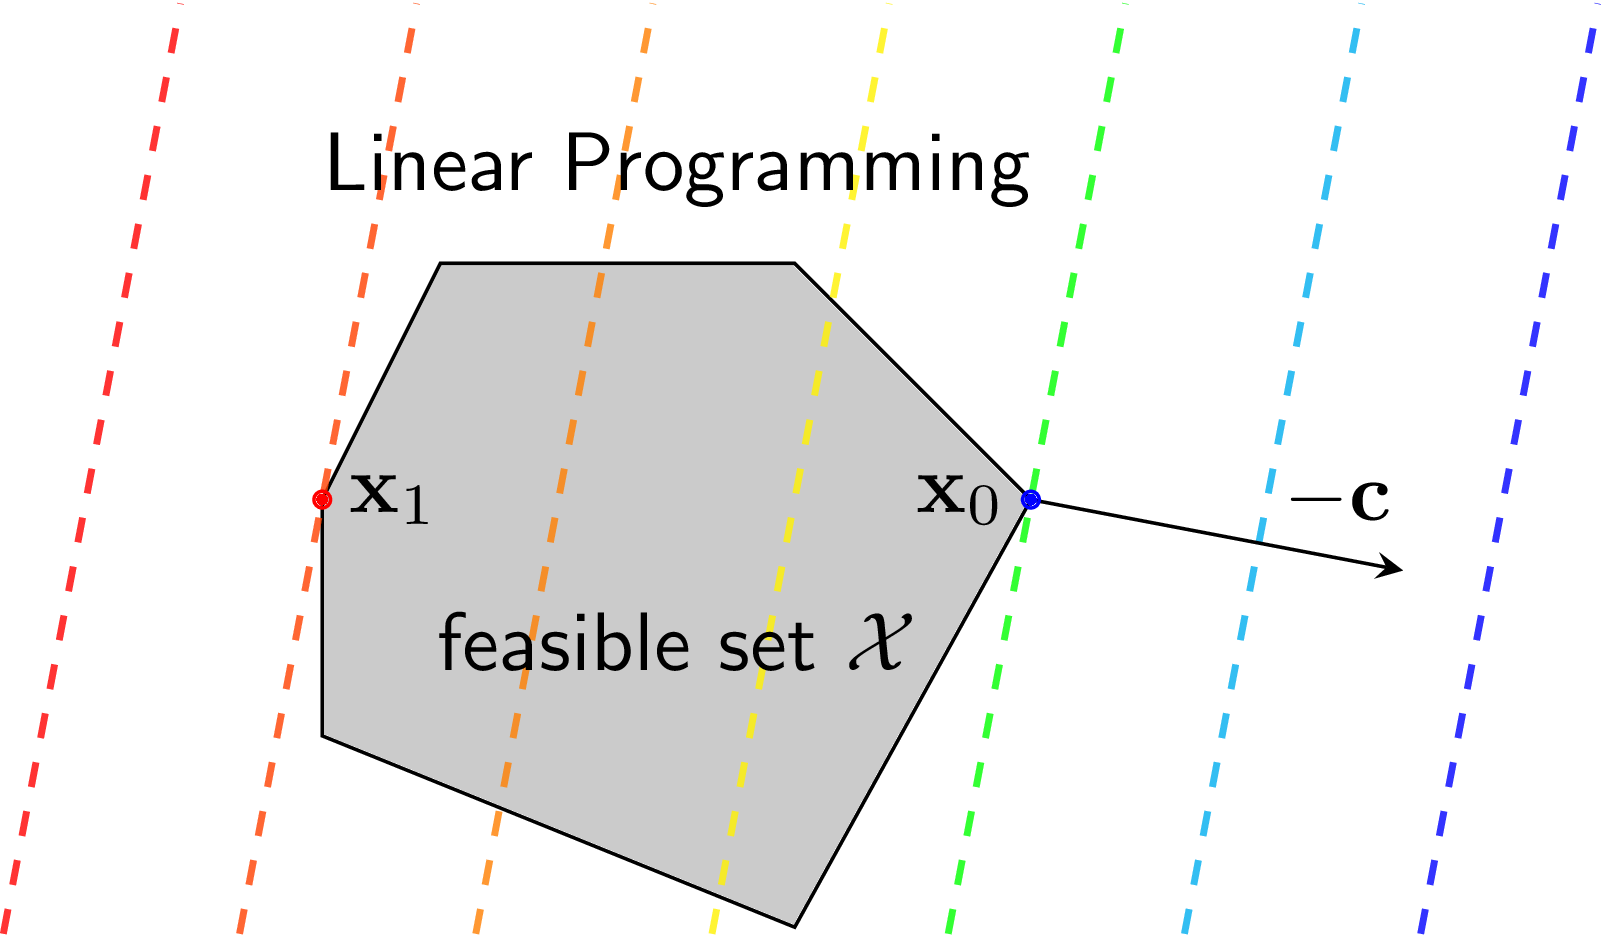
\includegraphics[scale=0.2]{lp.png}
    \end{center}
    \caption{Minh họa hình học bài toán Linear Programming}
    \label{refhinh1}
    \end{figure}
\end{center}
\subsubsection{Bài toán quy hoạch bậc hai (Quadractic Programming)}\\
\begin{mybox}
\begin{eqnarray}
\mathbf{x} &=& \arg\min_{\mathbf{x}} \frac{1}{2} \mathbf{x}^T\mathbf{P}\mathbf{x} + \mathbf{q}^T\mathbf{x} + \mathbf{r} \\
\text{Thỏa mãn:} &&\mathbf{Gx} \preceq \mathbf{h} \\
&& \mathbf{Ax} = \mathbf{b}
\end{eqnarray}
\end{mybox}
Trong đó: $P \in S^n_{+}$ (tập các ma trận vuông nửa xác định dương có số cột là n
), $G\in R^{m,n}, A \in R^{pxn}$.
\begin{center}
    \begin{figure}[H]
    \begin{center}
     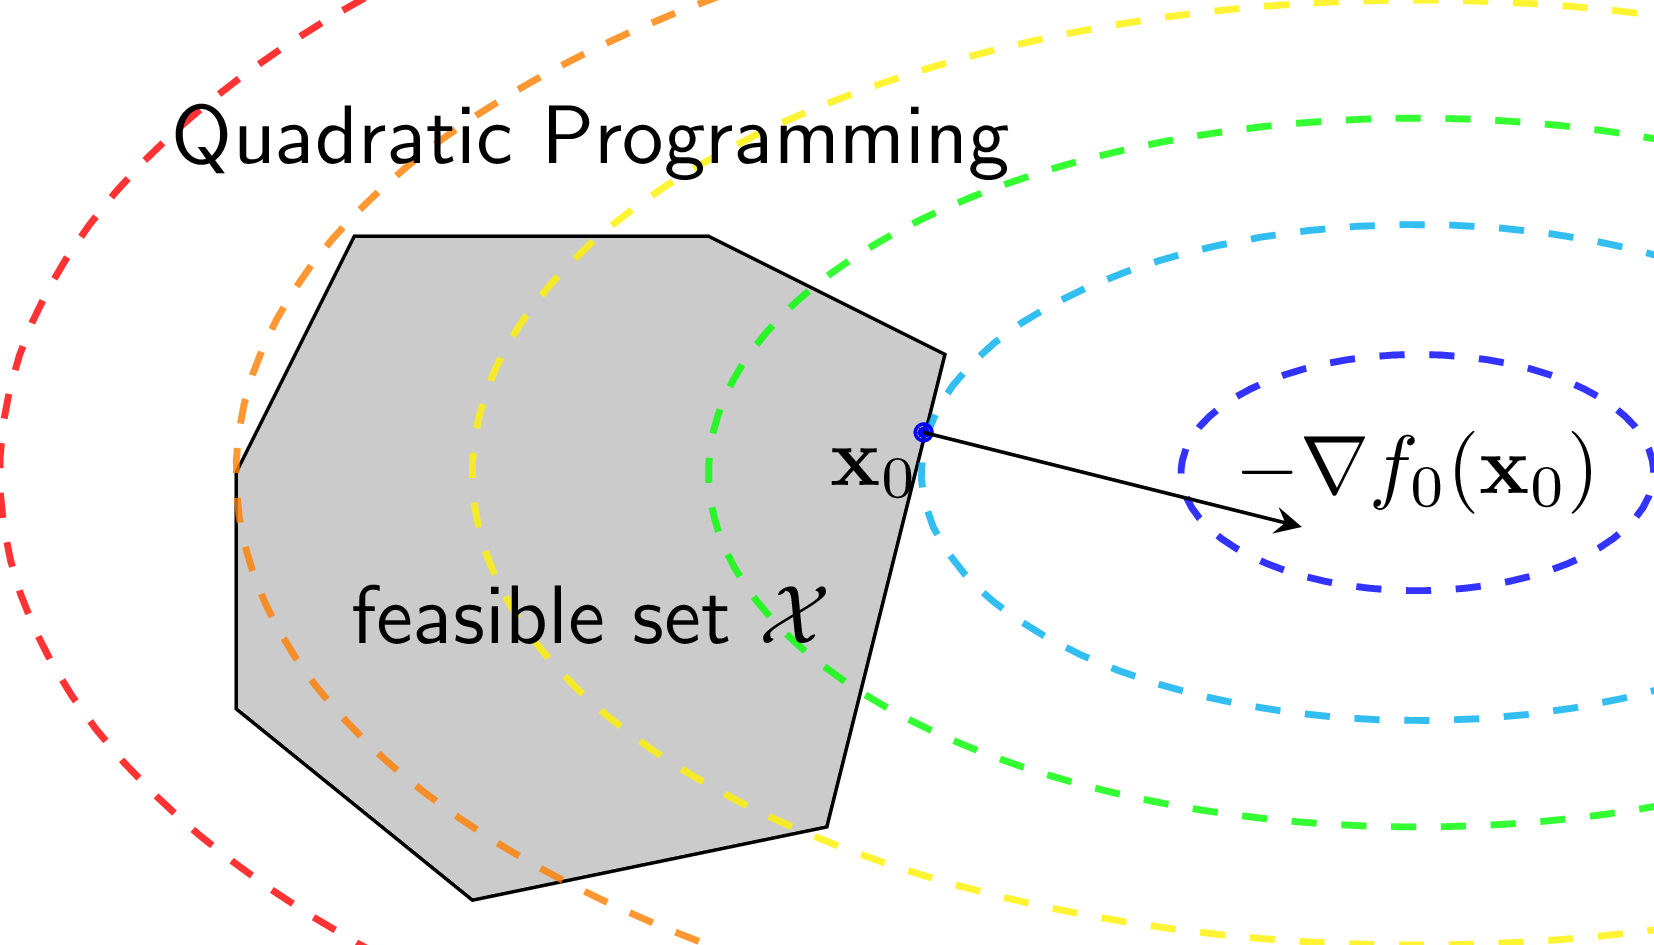
\includegraphics[scale=0.2]{qp.png}
    \end{center}
    \caption{Minh họa hình học bài toán Quadratic Programming}
    \label{refhinh1}
    \end{figure}
\end{center}
\subsection{Hướng giải các bài toán tối ưu lồi} 
Bài toán tổng quát: 
\begin{mybox}
$$ x^* = argmin_x f_0(x) $$
    Thỏa mãn: $$f_i(x) \leq 0 , i = 1,2,3...m$$
    $$h_j(x) = 0, j = 1,2,3..p$$
    $$ D = \cap_0^m (dom f_i) \cap \cap_1^p(don h_j) $$
\end{mybox}
Đôi khi giải \textbf{bài toán đối ngẫu} đơn giản hơn giải bài toán gốc nên đối với một số bài toán người ta tập trung vào giải bài toán đối ngẫu. Một bài toán ràng buộc có thể được đưa về bài toán đối ngẫu không ràng buộc bằng phương pháp nhân tử Lagrange. Nhân tử Lagrange được định nghĩa:
\begin{mybox}
$$ L(x,\lambda,\nu) = f_0(x) + \sum_{i=1}^{m}{\lambda_i f_i(x)} + \sum_{j=1}^{p}{\nu_j h_j(x)}$$
$$ \lambda = [\lambda_1, \lambda_2,...\lambda_m]$$
$$ \nu = [\nu_1,\nu_2,..\nu_p] $$
- Tổng số biến là: n+m+p\\
- Nếu L không bị chặn dưới: $g(\lambda,\nu) \rightarrow -\infty$\\
\end{mybox}
\textbf{Hàm đối ngẫu Lagrange} của bài toán tối ưu là một hàm của các biến đối ngẫu được định nghĩa là giá trị nhỏ nhất của $x$ của nhân tử Lagrange:
\begin{mybox}
$$ g(\lambda,\nu) = inf_{x\in D}L(x,\lambda,\nu) $$
$$ = inf_{x\in D}(f_0(x) + \sum_{i=1}^{m}{\lambda_i f_i(x)} + \sum_{j=1}^{p}{\nu_j h_j(x)})$$
- Nếu $p^*$ là giá trị tối ưu (optimal value) của bài toán tổng quát
, thì với các biến đối ngẫu $\lambda_i \geq 0$ và $\nu$ bất kỳ chúng ta sẽ có:
$g(\lambda,\nu) \leq p^*$
 bất kỳ, chúng ta sẽ có:
 $$g(\lambda, \nu) \leq p^*~~~~ $$
\end{mybox}
\textbf{Bài toán đối ngẫu} Với mỗi cặp $(\lambda,\nu)$, cho chúng ta một chặn dưới cho nghiệm tối ưu của bài toán tối ưu tổng quát, chúng ta cần tìm ra một chặn dưới tốt nhất cho giá trị tối ưu này. Đây là lý do của bài toán đối ngẫu ra đời. Bài toán đối ngẫu Lagrange được định nghĩa:
\begin{mybox}
$$ \lambda ^*, \nu ^* = argmax_{\lambda,\nu} g(\lambda,\nu) $$
Thỏa mãn: $$ \lambda \succeq 0 $$
\end{mybox}
\textbf{Weak Duality}: Gọi $d^*$ là nghiệm tối ưu của bài toán đối ngẫu. Với nhận xét về chặn dưới của nghiệm tối ưu của bài toán tổng quát ta có $d^* \leq p^*$. Điều kiện này được gọi là \textit{weak duality}. Có nhiều bài toán không thể tìm ra nghiệm tối ưu nhưng ít ra chúng ta có thể biết được chặn dưới của nghiệm này.\\ \\
\textbf{Strong Duality}: Nếu đẳng thức $d^* = p^*$ xảy ra, chúng ta gọi đây là \textit{Strong Duality}.\\ \\
Một điểm được gọi là \textit{strictly feasible} nếu:
 \begin{mybox}
 $$ f_i(x)<0, i=1,2,3...m, Ax = b$$
 \end{mybox}
 \textbf{Định lý Slater} Nếu tổn tại một điểm \textit{strictly feasible} và bài toán gốc là lồi thì \textit{strong duality} xảy ra.\\ \\
 \textbf{Hệ điều kiện KKT} Để giải bài toán đối ngẫu khi điều kiện về \textit{strong duality} thoả mãn, chúng ta giải hệ bất phương trình: 
\begin{mybox}
    $f_i(x^*) \leq 0, i = 1,2,...m$\\
    $h_j(x^*) = 0, j = 1,2,3,..p$\\
    $\lambda_i^* \geq 0, i = 1,2,..m$\\
    $\lambda_i^*f_i(x^*) = 0, i = 1,2,3...,m$\\
    $\nabla f_0(x^*) + \sum_{i=1}^{m}{\lambda_i^* \nabla f_i(x^*)} + \sum_{j=1}^{p}{\nu_j^* \nabla h_j(x^*)} = 0$
\end{mybox}
\subsection{Thư viện cvxopt}
CVXOPT là một thư viện miễn phí trên Python giúp giải rất nhiều bài toán tối ưu lồi. Tác giả của thư viện này, Lieven Vanderberghe là tác giả thứ hai của cuốn sách \textit{Convex Optimization}.
\subsubsection{Giải bài toán Linear Programming bằng thư viên cvxopt}
Bài toán Linear Programming dạng chuẩn tắc hoàn toàn có thể được lập trình để giải bằng thư viện cvxopt. 
Bài toán mẫu dạng chuẩn tắc: 
\begin{mybox}
\begin{eqnarray}
(x, y) =& \arg\max_{x, y} 5x + 3y \\
\text{thỏa mãn:}~ & x + y \leq 10 \\
                    & 2x + y \leq 16  \\
                    & x + 4y \leq 32 \\
                    & x, y \geq 0
\end{eqnarray}
\end{mybox}
Các điều kiện ràng buộc có thể viết lại dưới dạng $\mathbf{Gx} \preceq \mathbf{h}$ hay viết dưới dạng tường minh
$$\mathbf{G} = \left[\begin{matrix}
1 & 1 \\
2 & 1 \\
1 & 4 \\
-1 & 0 \\
0 & -1
\end{matrix}\right], ~~~~
\mathbf{h} = \left[\begin{matrix}
10\\
16 \\
32 \\
0 \\
0
\end{matrix}\right] $$
Bài toán Linear Programming có thể được giải bằng thư viện cvxopt thông qua đoạn code
\begin{lstlisting}
from cvxopt import matrix, solvers
c = matrix([-5., -3.])
G = matrix([[1., 2., 1., -1., 0.], [1., 1., 4., 0., -1.]])
h = matrix([10., 16., 32., 0., 0.])

solvers.options['show_progress'] = False
sol = solvers.lp(c, G, h)

print('Solution"')
print(sol['x'])
\end{lstlisting}
Nghiệm của bài toán sau khi lập trình tìm nghiệm bằng thư viện
\begin{lstlisting}
Solution:
[ 6.00e+00]
[ 4.00e+00]
\end{lstlisting}
\subsubsection{Giải bài toán Quadratic Programming bằng thư viên cvxopt}
Tương tự, bài toán Quadractic Programming dạng chuẩn tắc cũng hoàn toàn có thể được lập trình hỗ trợ bởi thư viện cvxopt. 
Bài toán mẫu dạng chuẩn tắc:Bài toán mẫu: 
 
\begin{mybox}
\begin{eqnarray}
(x, y) &=& \arg\min_{x, y} (x - 10)^2 + (y - 10)^2 \\
\text{subject to:}~&&
\left[\begin{matrix}
1 & 1 \\
2 & 1 \\
1 & 4 \\
-1 & 0 \\
0 & -1
\end{matrix}\right]
\left[
\begin{matrix}
x \\
y
\end{matrix}
\right]
\preceq
\left[\begin{matrix}
10\\
16 \\
32 \\
0 \\
0
\end{matrix}\right]
\end{eqnarray}
\end{mybox}
Bài toán Quadractic Programming có thể được giải bằng thư viện cvxopt thông qua đoạn code
\begin{lstlisting}
from cvxopt import matrix, solvers
P = matrix([[1., 0.], [0., 1.]])
q = matrix([-10., -10.])
G = matrix([[1., 2., 1., -1., 0.], [1., 1., 4., 0., -1.]])
h = matrix([10., 16., 32., 0., 0])

solvers.options['show_progress'] = False
sol = solvers.qp(P, q, G, h)

print('Solution:')
print(sol['x'])
\end{lstlisting}
Nghiệm của bài toán sau khi lập trình tìm nghiệm bằng thư viện
\begin{lstlisting}
Solution:
[ 5.00e+00]
[ 5.00e+00]
\end{lstlisting}


\chapter{Bài toán SVM trong học máy và phương pháp giải}

\section{Bài toán SVM (Support Vector Machine)} 
\subsection{Bài toán phân 2 lớp} 
\begin{center}
    \begin{figure}[H]
    \begin{center}
     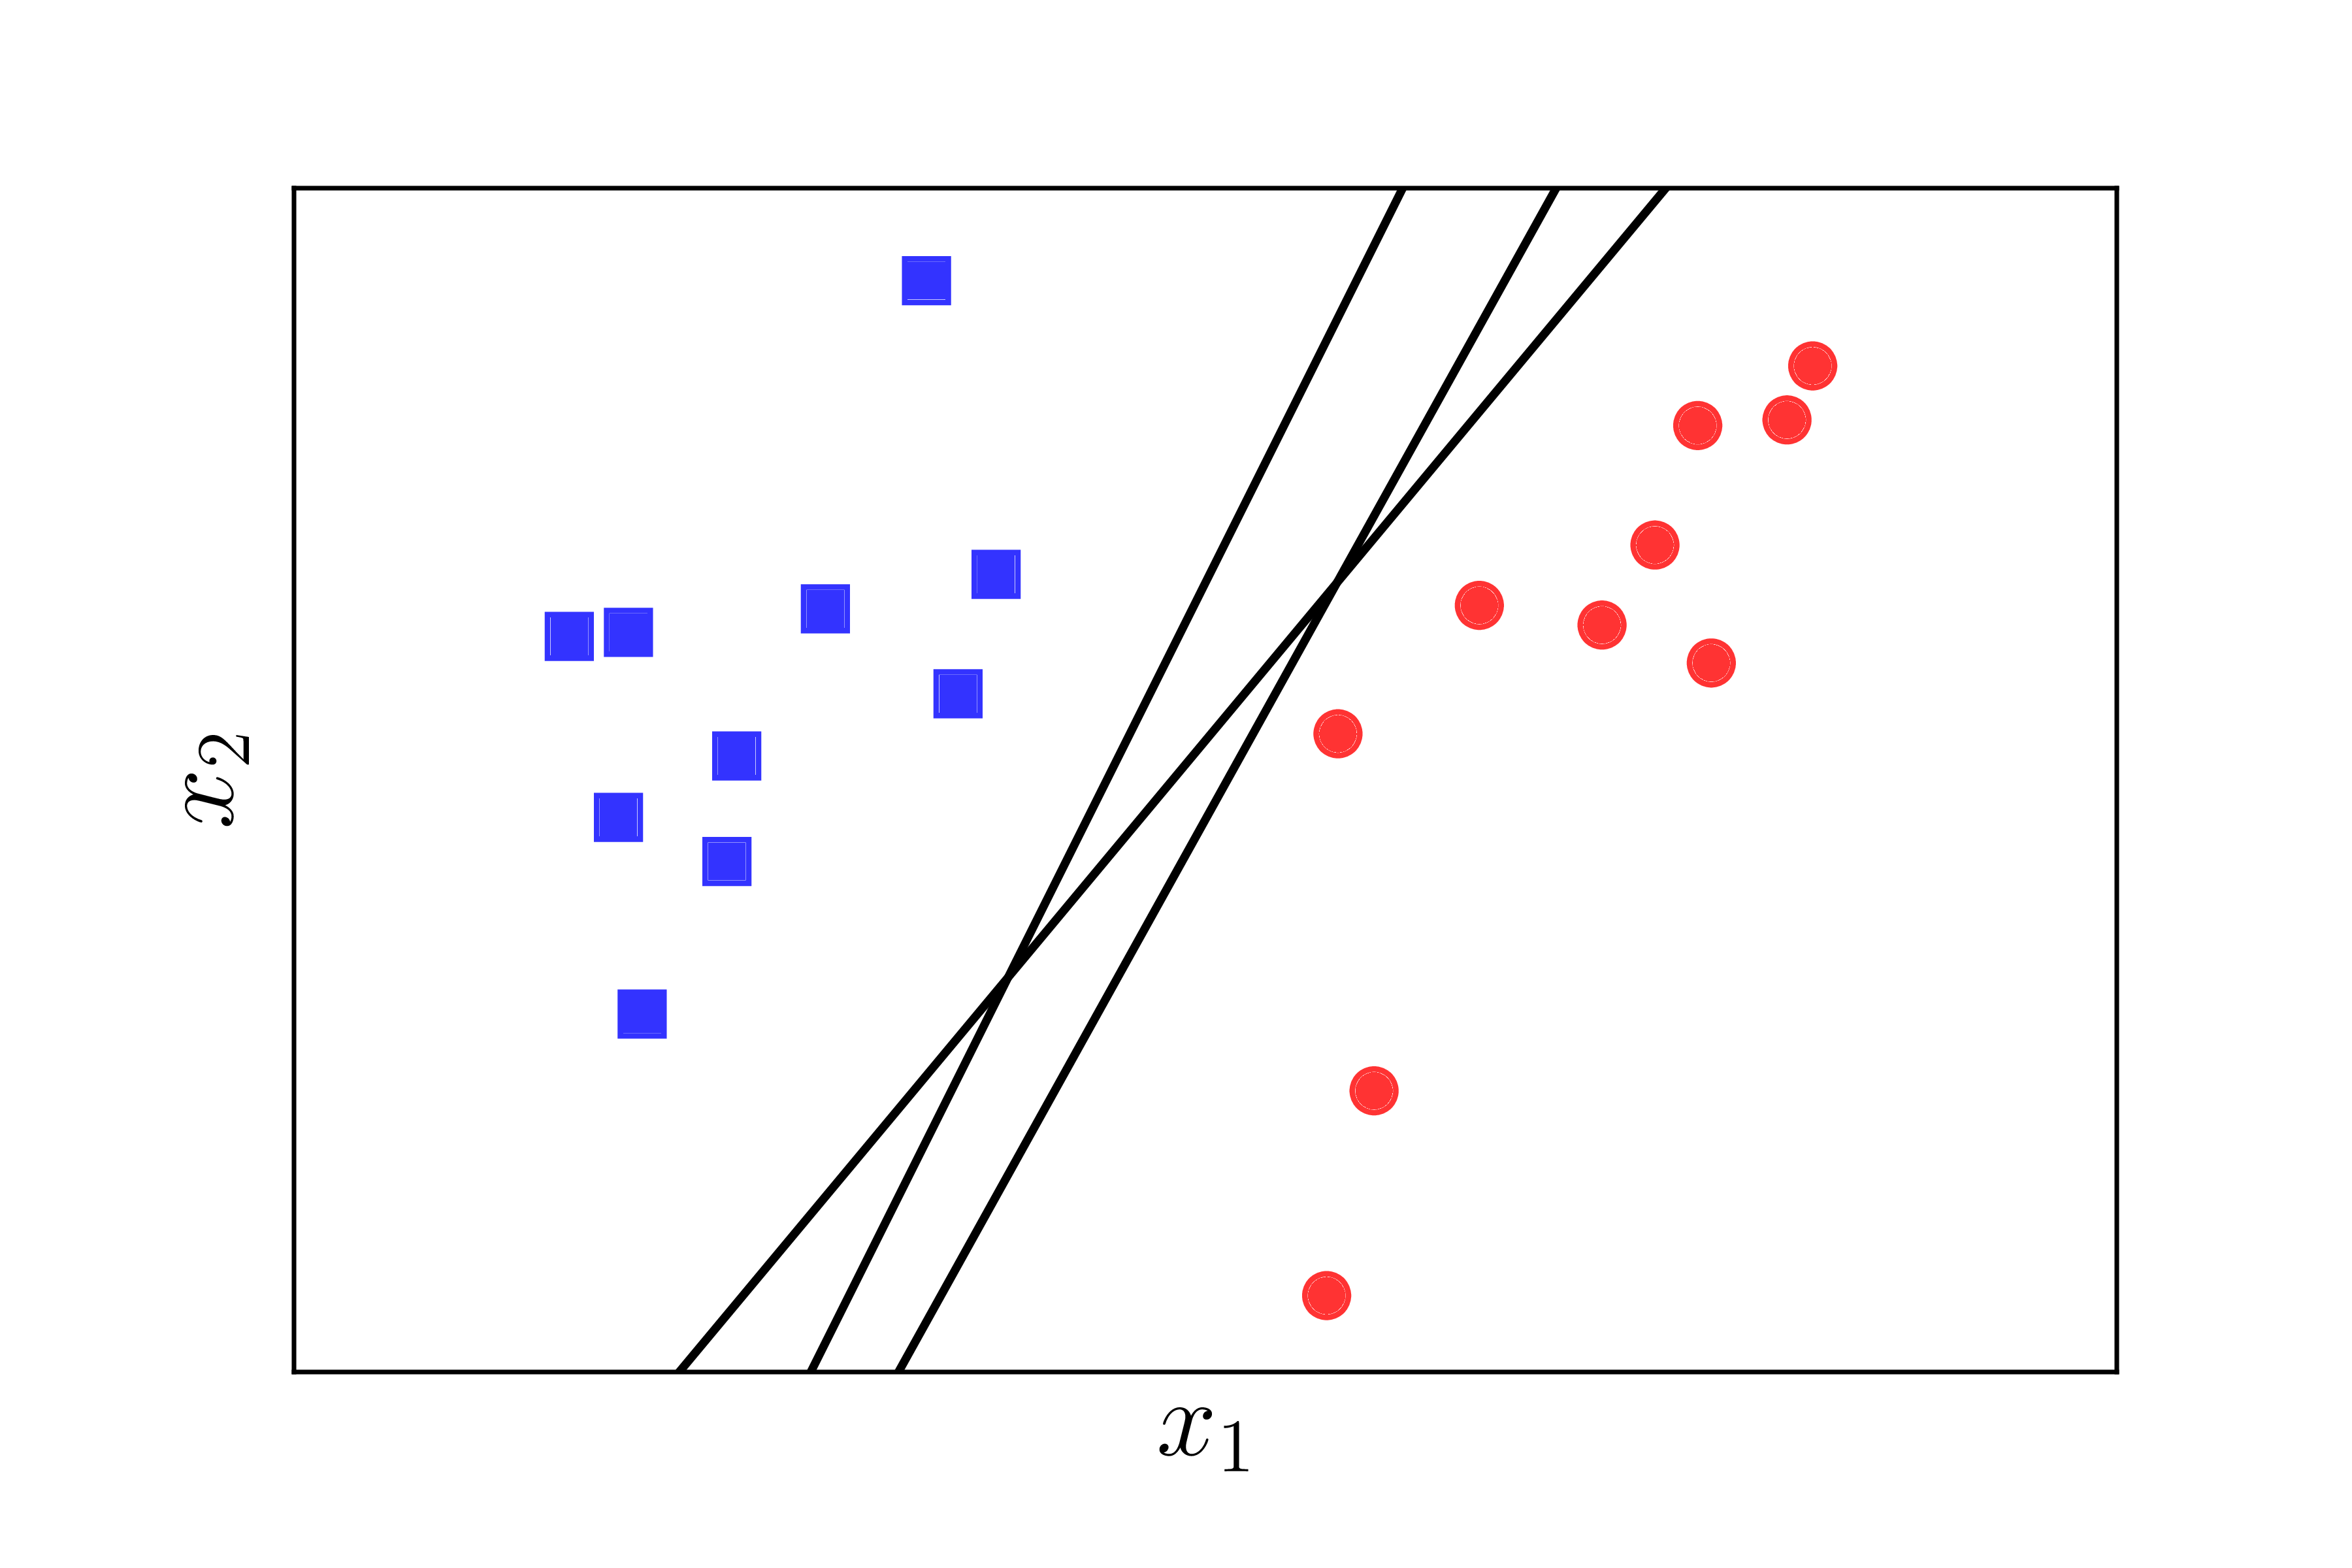
\includegraphics[scale=0.08]{svm1.png}
    \end{center}
    \caption{Minh họa dữ liệu khả tách tuyến tính}
    \label{refhinh1}
    \end{figure}
\end{center} 
Một số vấn đề thường gặp trong bài toán phân loại 2 lớp: 
\begin{itemize}
    \item Có nhiều đường thẳng thoả mãn tiêu chí phân được hai lớp.
    \item Có đường thẳng nào phân lớp được rạch ròi nhất giữa hai lớp mà vẫn đảm bảo sự công bẳng giữa hai lớp với nhau?
\end{itemize}
\textbf{Định nghĩa lề (margin)}: Khoảng cách từ điểm gần biên nhất đến biên.\\ \\
\textbf{Mục tiêu của bài toán SVM: }
\begin{itemize}
\item Sự công bằng được thể hiện ở hai lề của mỗi lớp phải giống nhau. \\ 
\item Sự rạch ròi được thể hiện ở sự tối đa hoá lề ở mỗi lớp. \\
\item Bài toán SVM ra đời để đáp ứng được hai tiêu chí công bằng và rạch ròi giữa  hai hay nhiều lớp.
\end{itemize}
\subsection{Bài toán Support Vector Machine (SVM)}
Bài toán SVM là bài toán tìm đường phân loại sao cho lề (margin) của hai hay nhiều lớp là lớn nhất. Bản chất SVM là một bài toán tối ưu. Ta sẽ xây dựng bài toán tối ưu cho bài toán SVM với quy ước tập dữ liệu là $(x_1,y_1),(x_2,y_2),(x_3,y_3),...(x_N,y_N)$ với nhãn là $y_1,y_2,y_3,...y_N$. Không mất tính tổng quát giả sử hai lớp có nhãn là 1 và -1. Với mỗi điểm $(x_i,y_i)$ trong tập dữ liệu, khoảng cách đến mặt phẳng phân cách được tính như sau:\\

\begin{mybox}
$$\frac{y_n(\mathbf{w}^T\mathbf{x}_n + b)}{||\mathbf{w}||_2}$$ \end{mybox}
Lề của mỗi lớp (class) được định nghĩa bằng công thức:
\begin{mybox}
$$\text{margin} = \min_{n} \frac{y_n(\mathbf{w}^T\mathbf{x}_n + b)}{||\mathbf{w}||_2}$$ 
\end{mybox}
\bigskip

Phát biểu bài toán SVM dưới dạng bài toán tối ưu và biến đổi toán học: 
\begin{mybox} $$
(\mathbf{w}, b) = \arg\max_{\mathbf{w}, b} \left\{
    \min_{n} \frac{y_n(\mathbf{w}^T\mathbf{x}_n + b)}{||\mathbf{w}||_2} 
\right\}
= \arg\max_{\mathbf{w}, b}\left\{
    \frac{1}{||\mathbf{w}||_2} \min_{n} y_n(\mathbf{w}^T\mathbf{x}_n + b)
\right\} )(2)$$  \end{mybox}
Nếu để nguyên gốc, bài toán SVM sẽ rất phức tạp, tuy nhiên chúng ta có thể đưa về dạng đơn giản hơn với nhận xét nếu thay $w$ bởi $kw$ và $b$ bởi $kb (k>0)$  thì mặt phân cách không thay đổi. Không mất tính tổng quát ta có thể giả sử: 
\begin{mybox} $$y_n(\mathbf{w}^T\mathbf{x}_n + b) = 1$$ \end{mybox}
Như vậy với mọi $n$ ta có: \\
\begin{mybox}
$$y_n(\mathbf{w}^T\mathbf{x}_n + b) \geq 1$$ \end{mybox}
Bài toán (2) có thể đưa được về dạng bài toán tối ưu có ràng buộc: 
\begin{mybox}
\begin{eqnarray}
    (\mathbf{w}, b) &=& \arg \max_{\mathbf{w}, b} \frac{1}{||\mathbf{w}||_2}   \\
    \text{Thỏa mãn:}~ && y_n(\mathbf{w}^T\mathbf{x}_n + b) \geq 1, \forall n = 1, 2, \dots, N 
\end{eqnarray} \end{mybox}
Với một chút biến đổi, ta có thể biến đổi thành: 
\begin{mybox}
\begin{eqnarray}
    (\mathbf{w}, b) &=& \arg \min_{\mathbf{w}, b} \frac{1}{2}||\mathbf{w}||_2^2   \\
    \text{Thỏa mãn:}~ && 1 - y_n(\mathbf{w}^T\mathbf{x}_n + b) \leq 0, \forall n = 1, 2, \dots, N ~~~~ (3)
\end{eqnarray}
\end{mybox}
 \begin{center}
    \begin{figure}[H]
    \begin{center}
     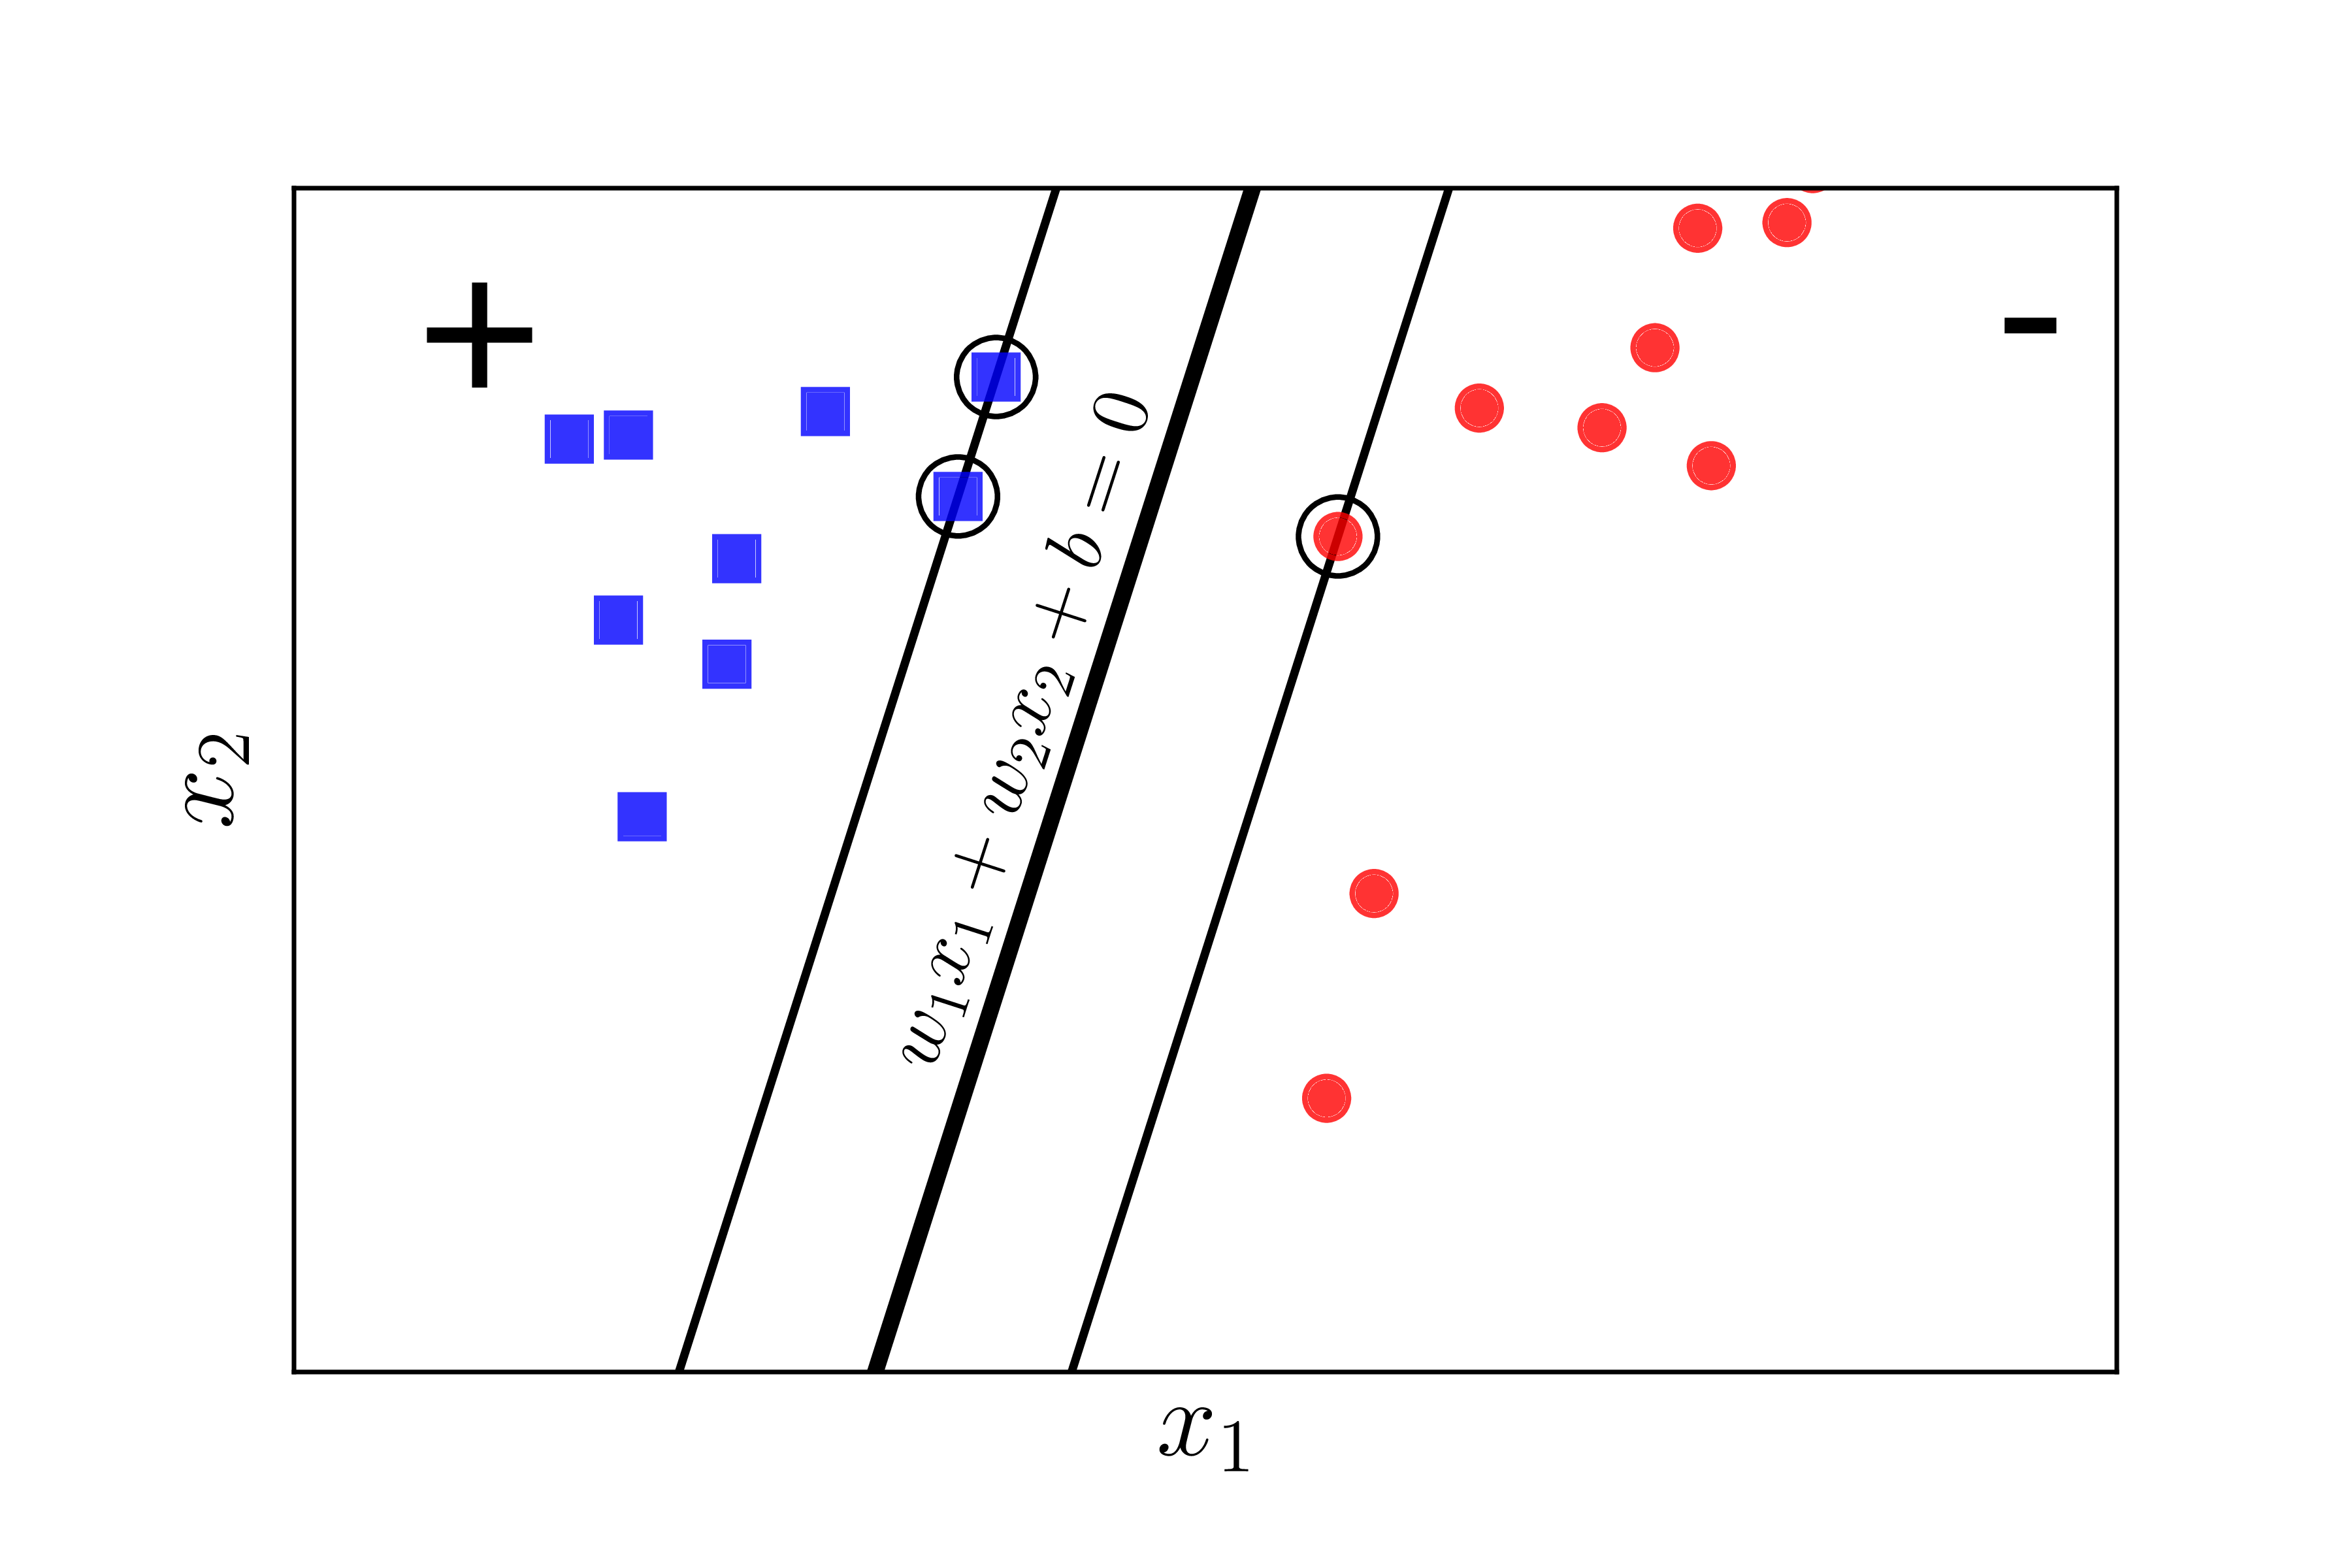
\includegraphics[scale=0.07]{svm6.png}
    \end{center}
    \caption{Minh họa nghiệm của mô hình SVM}
    \label{refhinh1}
    \end{figure}
\end{center} 
\section{Giải bài toán SVM }
\subsection{Giải bằng thư viện cvxopt} 
Bài toán (2.3) là một bài toán tối ưu lồi vì hàm mục tiêu là hàm Norm. Hơn nữa hàm mục tiêu là lồi nghiêm ngặt vì  $||\mathbf{w}||_2^2 =  \mathbf{w}^T\mathbf{I}\mathbf{w}$ với I là ma trận đơn vị và ma trận nửa xác định dương, do đó bài toán có nghiệm thì nghiệm đó là duy nhất, và bài toán có thể giải được bằng thư viện cvxopt.
\subsection{Giải bằng bài toán đối ngẫu}
Lagrangian của bài toán (2.3):
\begin{mybox}
\begin{center}
$$\mathcal{L}(\mathbf{w}, b, \lambda) = \frac{1}{2} ||\mathbf{w}||_2^2 + \sum_{n=1}^N \lambda_n(1 - y_n(\mathbf{w}^T\mathbf{x}_n + b) )$$
Với $\lambda = [\lambda_1, \lambda_2, \dots, \lambda_N]^T$ và $\lambda_n \geq 0, ~\forall n = 1, 2, \dots, N$ \\
Hàm đối ngẫu: $g(\lambda) = \min_{\mathbf{w}, b} \mathcal{L}(\mathbf{w}, b, \lambda)$ với $\lambda \succeq 0$ \\
\end{center}
\end{mybox}
Bài toán đối ngẫu: 
\begin{mybox}
\begin{eqnarray}
     \lambda &=& \arg \max_{\lambda} g(\lambda)   \\
     \text{Thỏa mãn:}~ && \lambda \succeq 0\\
     && \sum_{n=1}^N \lambda_ny_n = 0 
 \end{eqnarray} \end{mybox}
Hệ điều kiện KKT: 
 \begin{mybox}
 \begin{eqnarray}
1 - y_n(\mathbf{w}^T\mathbf{x}_n + b) &\leq& 0, ~ \forall n = 1, 2, \dots, N \\
\lambda_n &\geq& 0, ~\forall n = 1, 2, \dots, N  \\
\lambda_n (1 - y_n(\mathbf{w}^T\mathbf{x}_n + b)) &=& 0, ~\forall n = 1, 2, \dots, N  \\
 \mathbf{w} &=& \sum_{n=1}^N \lambda_n y_n \mathbf{x}_n \\ 
 \sum_{n=1}^N \lambda_ny_n &=& 0
\end{eqnarray} \end{mybox}
Nhận thấy từ (2.11) suy ra với $n$ bất kỳ hoặc $\lambda_n = 0 $ hoặc $w^Tx + b =y_n ~~~~~~~~~~~~~~~~(2.13)$
Những điểm thoả mãn (2.13) là những điểm gần mặt phân cách nhất (support vectors). Những điểm này thường ít hay nói cách khác đa số $\lambda$ bằng 0. Tiếp tục phân tích, với những bài toán có số điểm dữ liệu $N$ nhỏ, ta có thể giải hệ điều kiện KKT phía trên bằng cách xét các trường hợp $\lambda = 0$ hoặc $\lambda_n \neq 0$. Tổng số trường hợp phải xét là $2^N$. Với $N > 50$, đây là một con số rất lớn, giải bằng cách này sẽ không khả thi. 

\subsection{Kết quả khi giải bằng thư viện thư viện cvxopt}
Sau khi tìm được $\lambda$ từ thư viện cvxopt, ta quan tâm đến những giá trị $\lambda_n \neq 0$. 
- Gọi $\mathcal{S} = \{n: \lambda_n \neq 0\}$ và $N_S$ là số phần tử của tập S. Với mỗi n ta có:
\begin{mybox}
$$1 = y_n(\mathbf{w}^T\mathbf{x}_n + b) \Leftrightarrow b + \mathbf{w}^T\mathbf{x}_n = y_n$$ \end{mybox}
Tính được: \begin{mybox} $$\mathbf{w} = \sum_{m \in \mathcal{S}} \lambda_m y_m \mathbf{x}_m ~~~~~~~~~~~~~~~~~~~ (2.14)$$ \end{mybox}
Từ đó có thể suy ra: 
\begin{mybox}
$$ b = \frac{1}{N_{\mathcal{S}}} \sum_{n \in \mathcal{S}}(y_n - \mathbf{w}^T\mathbf{x}_n) = \frac{1}{N_{\mathcal{S}}} \sum_{n \in \mathcal{S}} \left(y_n - \sum_{m\in \mathcal{S}} \lambda_m y_m \mathbf{x}_m^T \mathbf{x}_n\right)~~~~~ (2.15)$$ 
\end{mybox}
\section{Bài toán \textit{soft margin} SVM}
\subsection{Ưu điểm của bài toán SVM}
So với bài toán các mô hình phân lớp khác, mô hình SVM cho chúng ta một đường phân lớp tối ưu hơn về khoảng cách từ điểm gần đường phân lớp nhất đến đường phân lớp (biên). Nghiệm của bài toán SVM cũng được chứng minh được tính đúng đắn bằng tối ưu hóa toán học. Do đó mô hình được sử dụng khá phổ biến trong thực tế.\\
\subsection{Hạn chế của bài toán SVM}

\begin{center}
    \begin{figure}[H]
    \begin{center}
     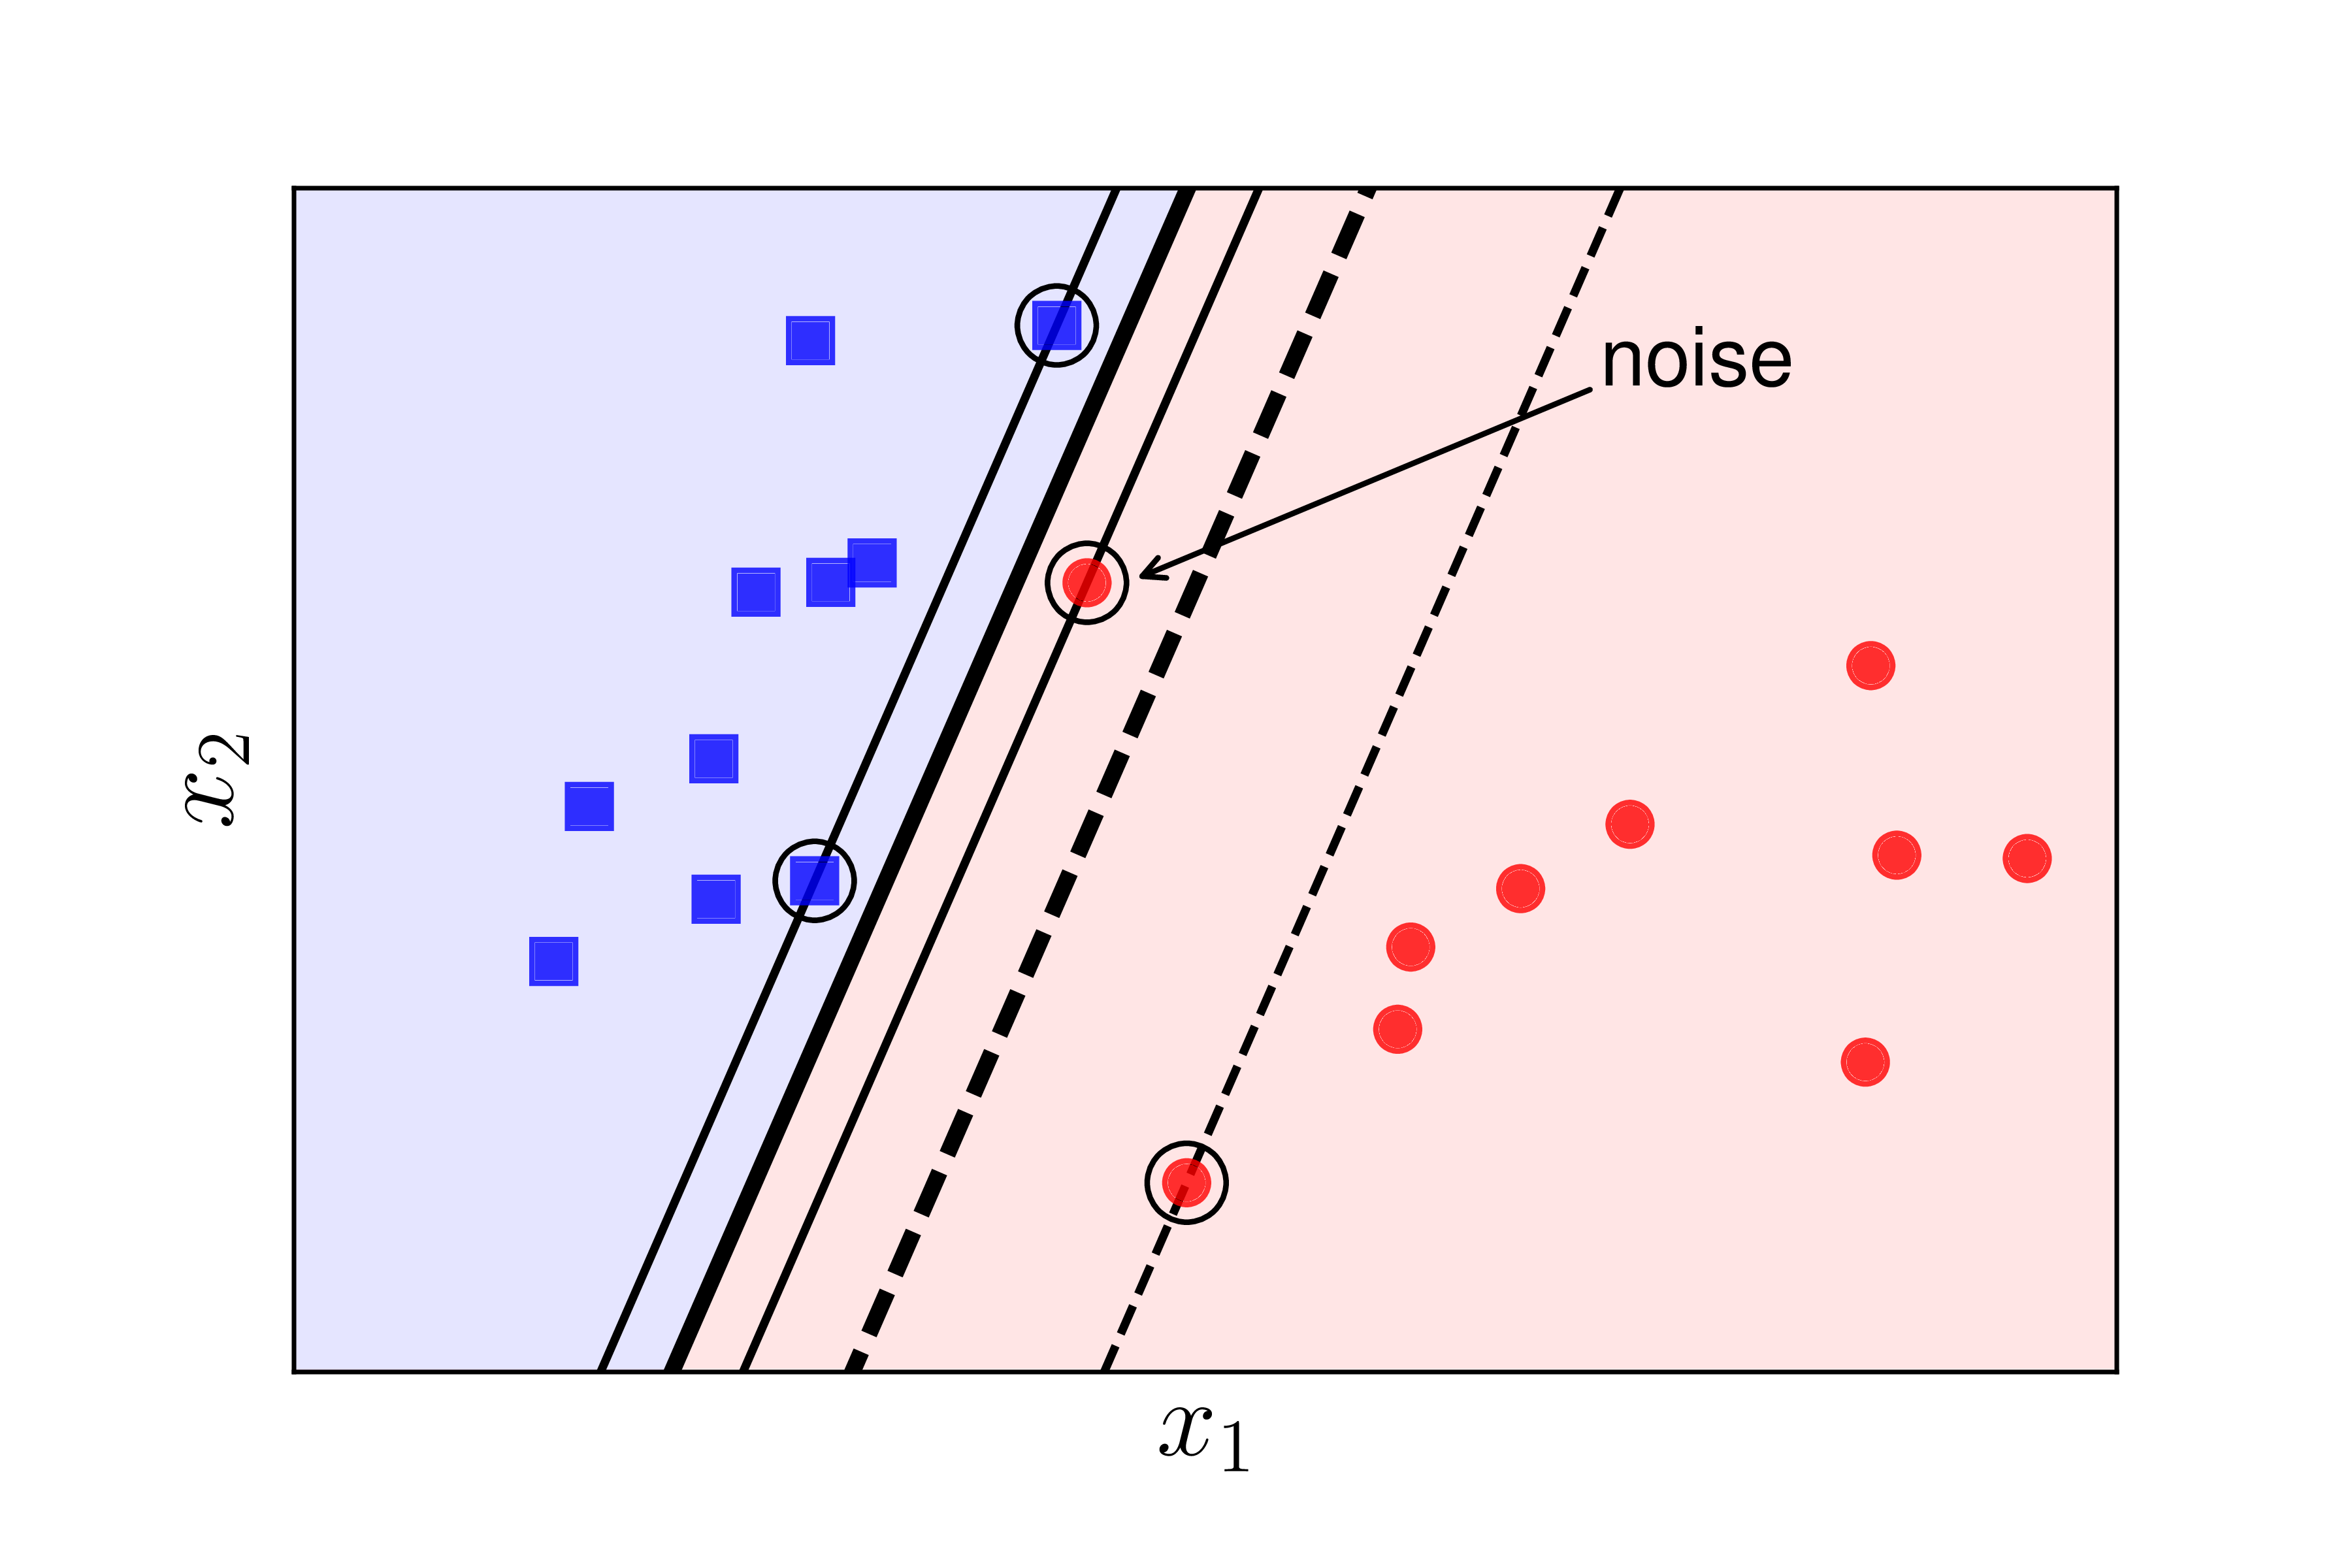
\includegraphics[scale=0.1]{ssvm1.png}
    \end{center}
    \caption{Minh họa điểm nhiễu làm cho lề quá nhỏ}
    \label{Hình 2.3}
    \end{figure}
\end{center} 
Dựa vào Hình \ref{Hình 2.3} ta thấy, khi dữ liệu có một điểm nhiễu (điểm màu đỏ trong hình), làm cho lề trở nên nhỏ và mặt phân chia gần điểm lớp màu xanh hơn lớp màu đỏ. Nhận xét rằng nếu hy sinh điểm nhiễu này chúng ta có thể có được mặt phân chia tốt hơn nhiều. 

\begin{center}
    \begin{figure}[H]
    \begin{center}
     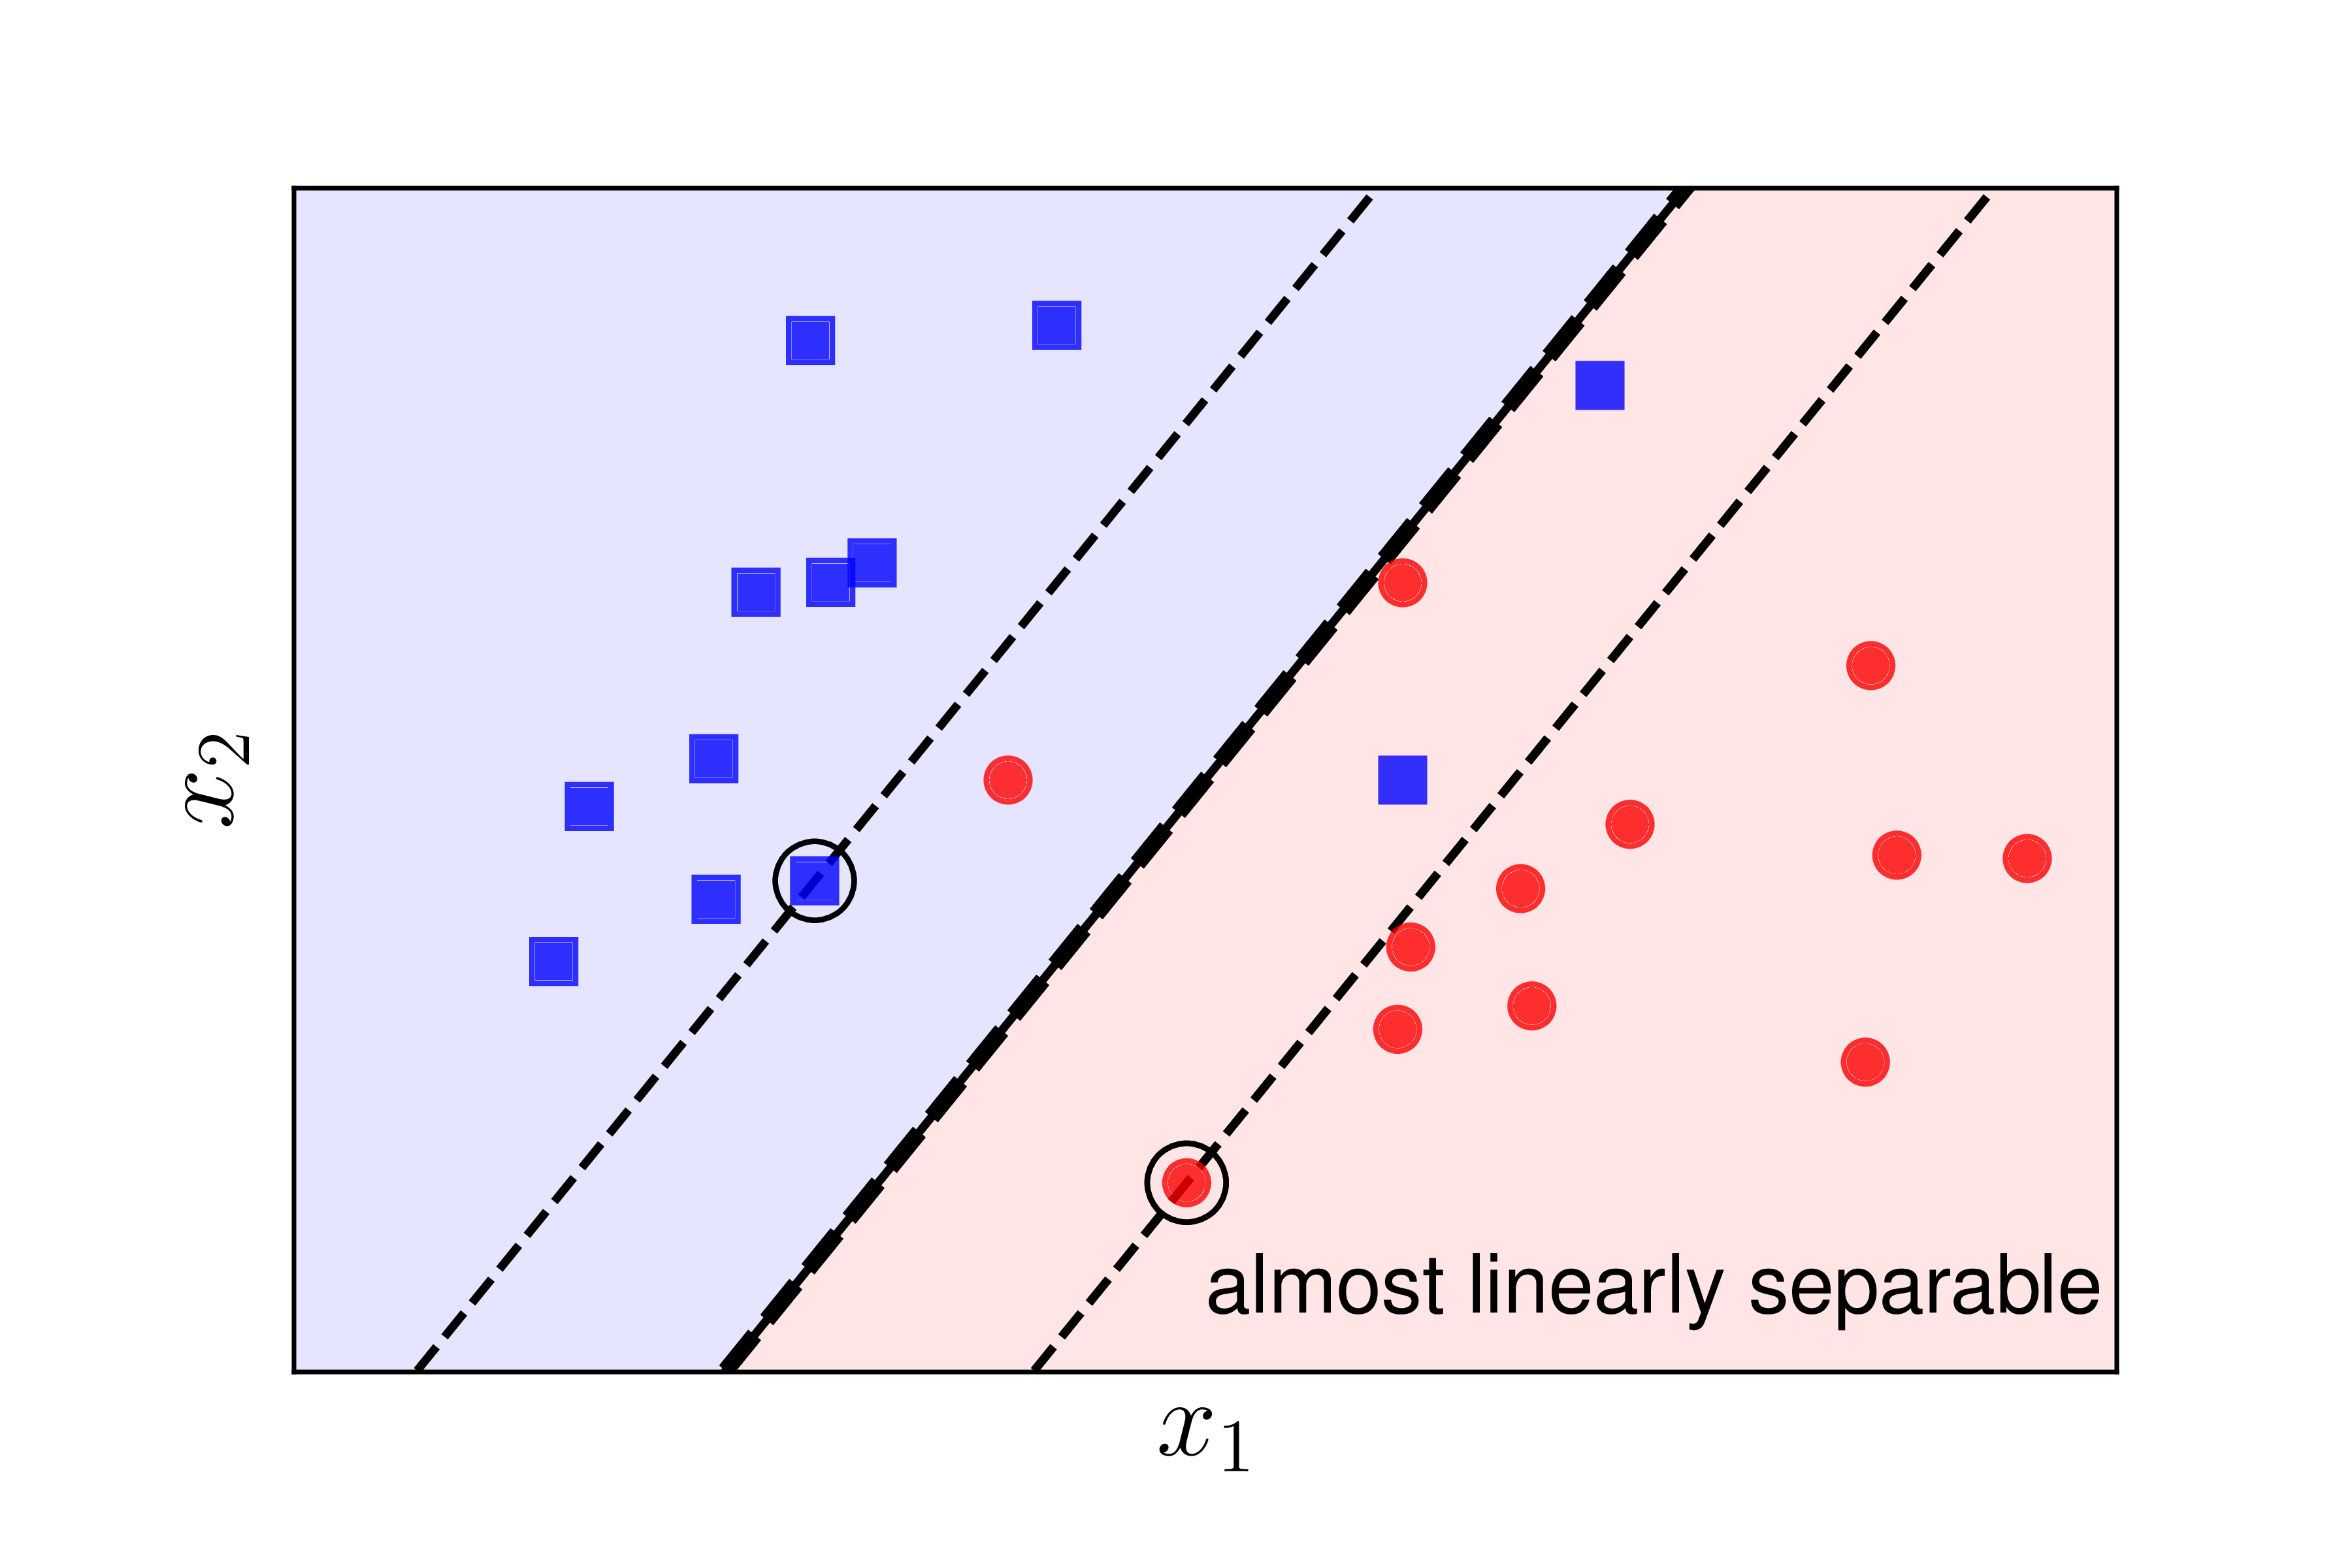
\includegraphics[scale=0.1]{ssvm2.png}
    \end{center}
    \caption{ Minh họa dữ liệu gần như khả tách tuyến tính}
    \label{Hình 2.4}
    \end{figure}
\end{center} 
 Trong trường hợp được mô tả ở Hình \ref{Hình 2.4}, nếu ta sử dụng mô hình SVM thuần thì rõ ràng bài toán tối ưu vô nghiệm. Tuy nhiên, nếu ta lại chịu hy sinh một chút những điểm ở gần biên giữa hai lớp (class/classes), ta vẫn có thể tạo được một đường phân chia khá tốt như đường nét đứt đậm. Các đường \textit{support} đường nét đứt mảnh vẫn giúp tạo được một lề (margin) lớn cho bộ phân lớp này. Với mỗi điểm nằm lần sang phía bên kia của các đường \textit{support} (hay đường \textit{margin}, hoặc đường biên) tương ứng, ta gọi điểm đó rơi vào vùng không an toàn. Chú ý rằng vùng an toàn của hai lớp là khác nhau, giao nhau ở phần nằm giữa hai đường \textit{support}.
 \subsection{Bài toán Soft margin SVM}
 Trong cả hai trường hợp trên, lề tạo bởi đường phân chia và đường nét đứt mảnh còn được gọi là lề mềm (soft margin). Cũng theo cách gọi này, SVM thuần còn được gọi là SVM lề cứng (hard margin SVM). Chúng ta có phân tích toán học: chúng ta cần hy sinh một vài điểm dữ liệu bằng cách chấp nhận cho chúng rơi vào vùng không an toàn. Tất nhiên, chúng ta phải hạn chế sự hy sinh này, nếu không, chúng ta có thể tạo ra một lề cực lớn bằng cách hy sinh hầu hết các điểm. Vậy hàm mục tiêu nên là một sự kết hợp để tối đa lề và tối thiểu sự hy sinh.
 \begin{center}
    \begin{figure}[H]
    \begin{center}
     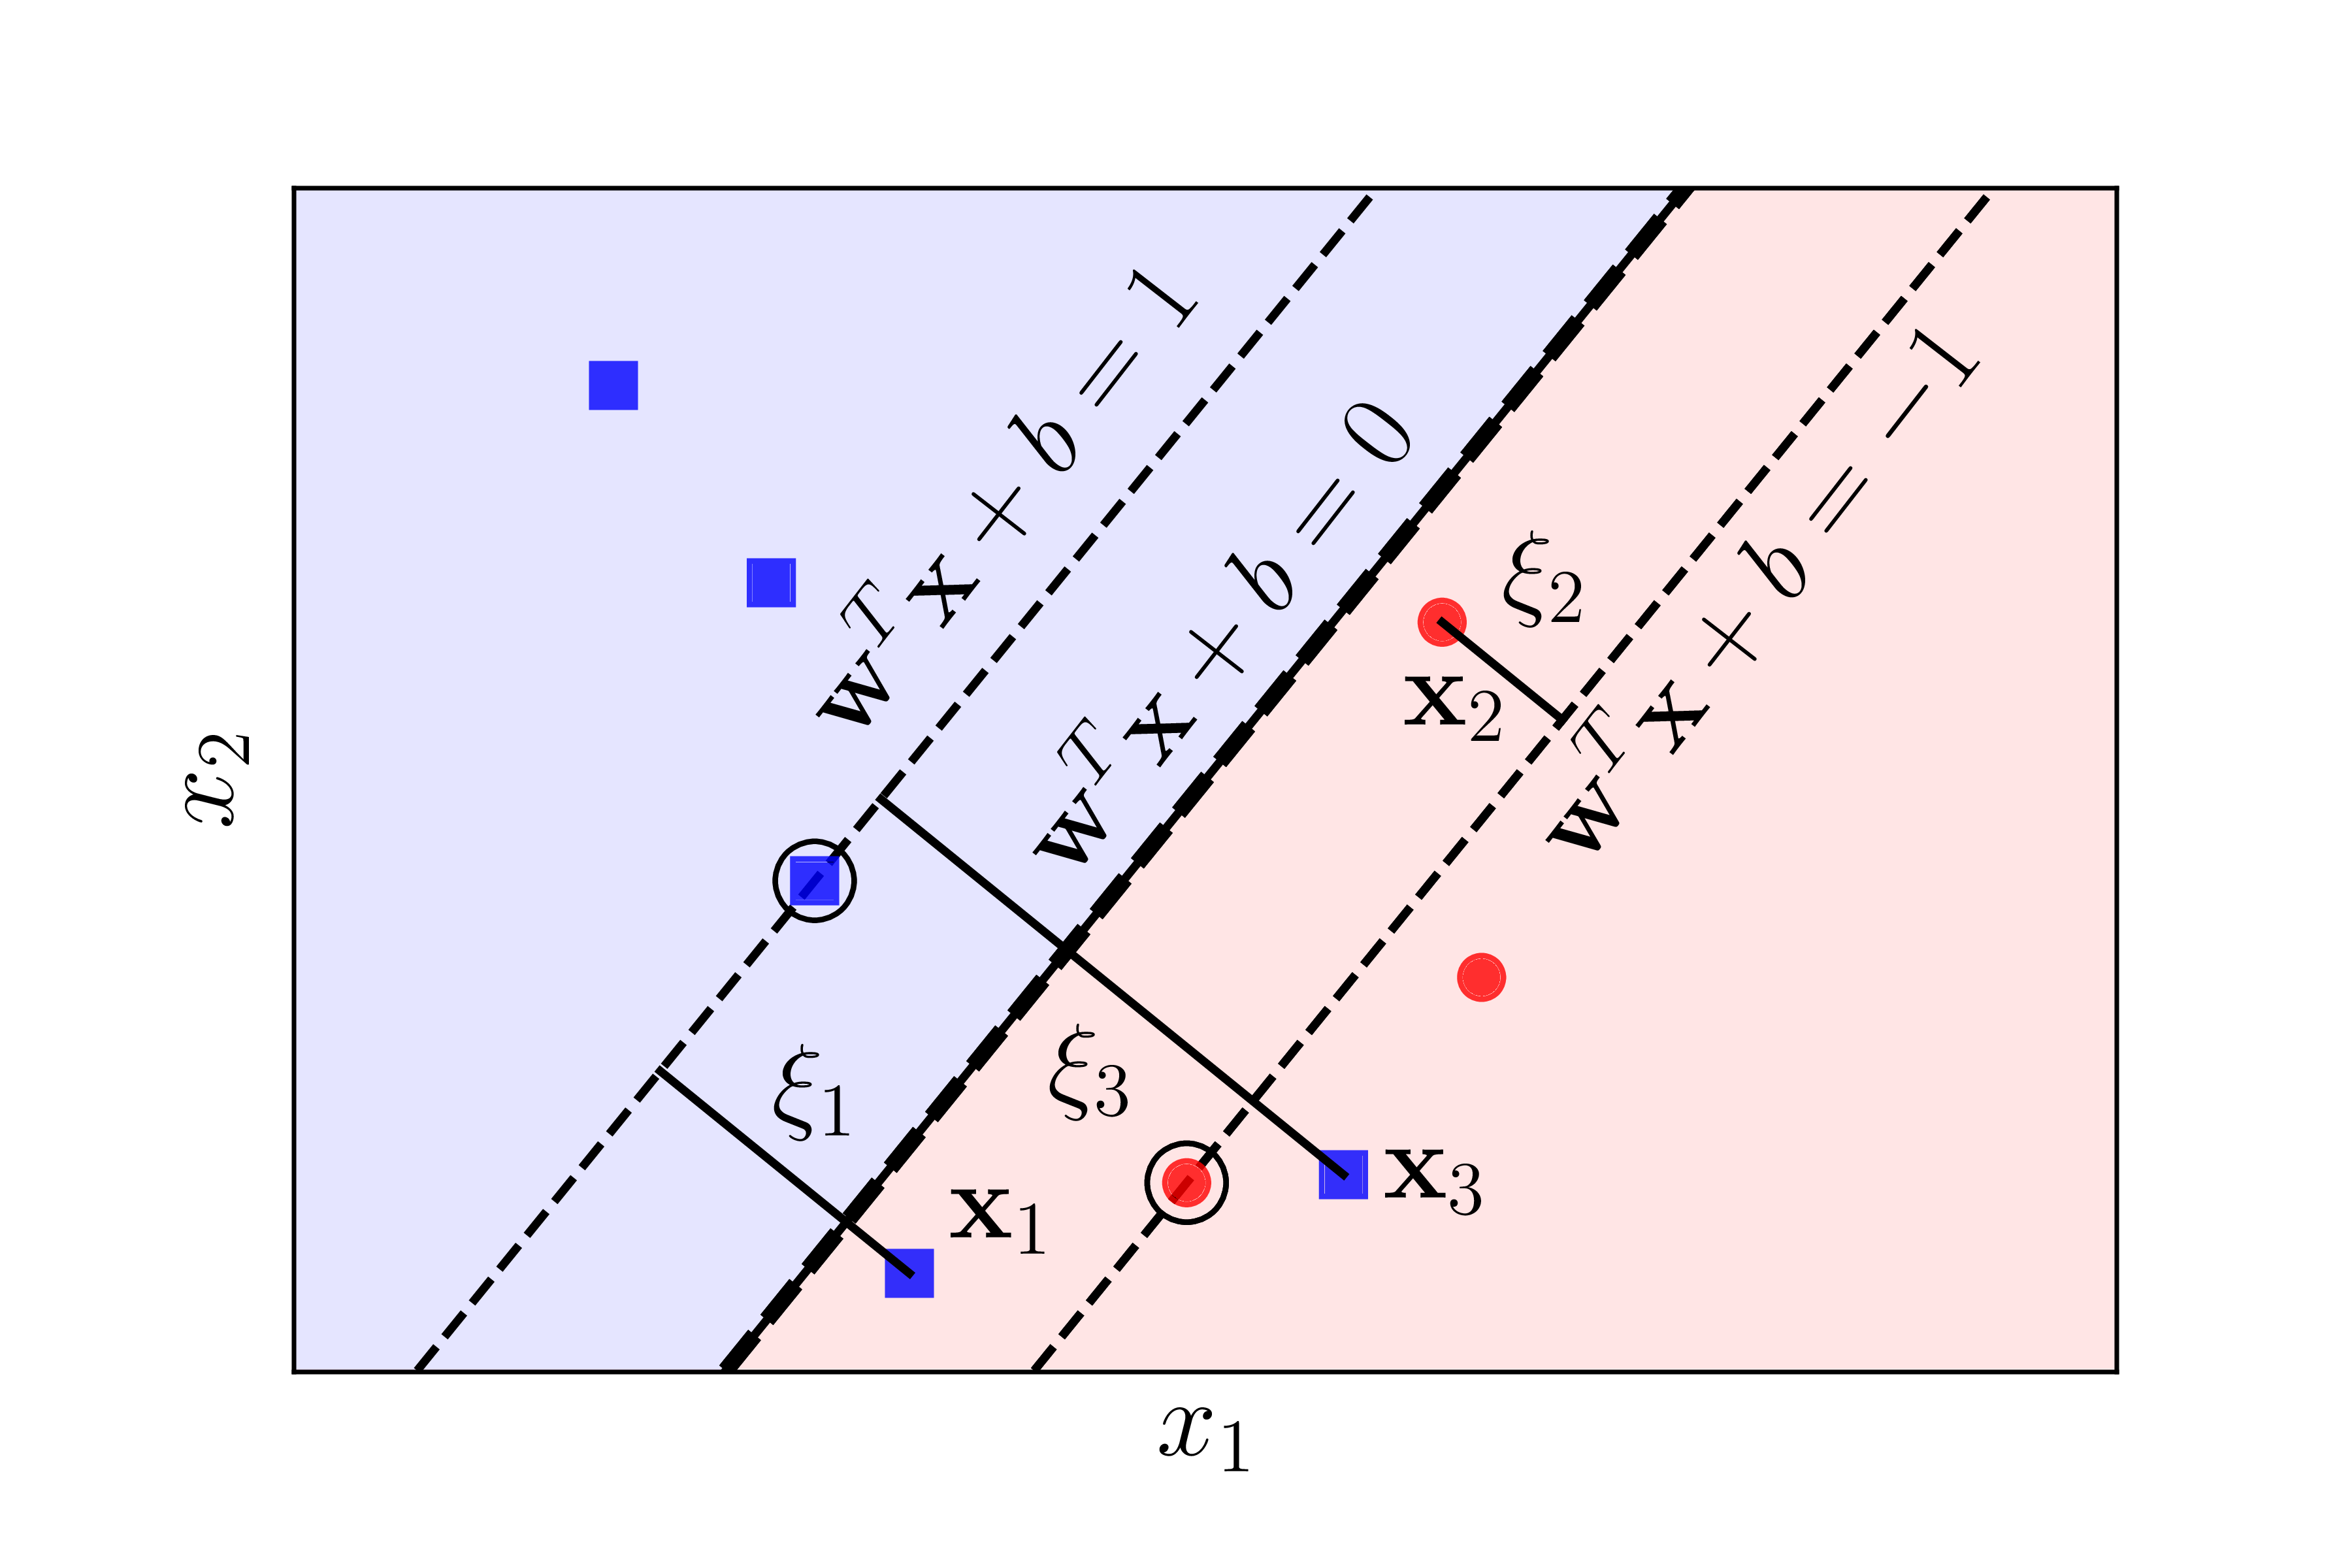
\includegraphics[scale=0.08]{ssvm3.png}
    \end{center}
    \caption{Minh họa biến $\xi_n$ đo sự hy sinh}
    \label{hình 2.5}
    \end{figure}
\end{center}
Để đo mức độ hy sinh mỗi điểm trong tập dữ liệu, ta sử dụng thêm một tham số $\xi_n$. Nếu $\xi_n = 0$, điểm đó đang nằm trong vùng an toàn. Nếu $\xi_n >0$, điểm đó đang nằm trong vùng không an toàn (như 3 điểm $x1,x2,x3$ trong Hình \ref{hình 2.5}) 
\subsection{Xây dựng bài toán tối ưu} 
Bài toán Soft margin có thể áp dụng: 
\begin{mybox}
\begin{eqnarray}
    (\mathbf{w}, b, \xi) &=& \arg \min_{\mathbf{w}, b, \xi} \frac{1}{2}{||\mathbf{w}||_2^2} + C \sum_{n=1}^N \xi_n  \\
    \text{Thỏa mãn:}~ && 1 - \xi_n - y_n(\mathbf{w}^T\mathbf{x}_n + b) \leq 0, \forall n = 1, 2, \dots, N \\
    && -\xi_n \leq 0,  ~\forall n = 1, 2, \dots, N
\end{eqnarray}
\end{mybox}
Hằng số $C$ được dùng để điều chỉnh tầm quan trọng giữa lề và sự hy sinh các điểm trong tập dữ liệu.\\ \\
Ký hiệu vector $\xi_n = [\xi_1,\xi_2,...,\xi_n]$\\
Chú ý ràng buộc mềm thay đổi từ bài toán gốc:
\begin{mybox}
$$y_n(\mathbf{w}^T\mathbf{x}_n + b) \geq 1 - \xi_n \Leftrightarrow 1 - \xi_n - y_n(\mathbf{w}^T\mathbf{x}_n + b) \leq 0, ~~ \forall n = 1, 2, \dots, n$$
\end{mybox}
Nhận xét: Nếu $\xi_n >0$ thì điểm đó rơi vào không an toàn. Nếu $C$ lớn, bài toán (25) sẽ tập trung vào tổi thiểu các biến đo sự hy sinh. Nếu $C$ càng lớn thì $\xi_n \rightarrow 0$ bài toán sẽ không có điểm nào phải hy sinh, bài toán trở thành bài toán SVM nguyên gốc. Ngược lại nếu $C$ nhỏ, bài toán sẽ tập trung vào việc tối thiểu $||w||_2^2$, hay tối đa lề, kéo theo biến hy sinh cũng lớn theo. 
\subsection{Giải bài toán soft margin bằng phương pháp gradient descent}
\textbf{Biến đổi từ bài toán ràng buộc thành không ràng buộc}\\ \\
Ràng buộc của bài toán (2.13) có thể được biến đổi như sau: 
\begin{mybox}
$$ \xi_n \geq 1 - y_n(\mathbf{w}^T\mathbf{x}_n + b) $$ 
\end{mybox}
Hơn nữa $\xi_n \geq 0$ do đó bài toán (2.13) có thể viết dưới dạng: 
\begin{mybox}
\begin{eqnarray}
    (\mathbf{w}, b, \xi) &=& \arg \min_{\mathbf{w}, b, \xi} \frac{1}{2}{||\mathbf{w}||_2^2} + C \sum_{n=1}^N \xi_n  \\
    \text{Thỏa mãn:}~ && \xi_n \geq max(0,1 -y_n(\mathbf{w}^T\mathbf{x}_n + b)), \forall n = 1, 2, \dots, N 
\end{eqnarray}
\end{mybox}
Nhận xét nếu $(w,b,\xi)$ là nghiệm của bài toán (2.13) thì:
\begin{mybox}
$$\xi_n = max(0,1 - y_n(\mathbf{w}^T\mathbf{x}_n + b)), \forall n= 1,2,...N$$ \end{mybox}
- Thật vậy, giả sử tồn tại n sao cho: $\xi_n > max(0,1 - y_n(\mathbf{w}^T\mathbf{x}_n + b))$. Ta chọn $\xi_n' = max(0,1 - y_n(\mathbf{w}^T\mathbf{x}_n + b))$ khi đó, tất cả ràng buộc của bài toán vẫn được thoả mãn trong khi ta thu được giá trị của hàm mục tiêu thấp hơn (mâu thuẫn). Khi đó bài toán trở thành bài toán tối ưu không ràng buộc: \\ 
\begin{mybox}
\begin{eqnarray}
    (\mathbf{w}, b, \xi) &=& \arg \min_{\mathbf{w}, b, \xi} \frac{1}{2}{||\mathbf{w}||_2^2} + C \sum_{n=1}^N {max(0,1 - y_n(\mathbf{w}^T\mathbf{x}_n + b))}  
\end{eqnarray}
\end{mybox}
\textbf{Hinge Loss}\\ \\
Giới thiệu Hinge Loss: 
\begin{mybox}
$$J_n(w,b) = max(0, 1 -y_nz_n)$$
\end{mybox}
Trong đó: $z_n$ là \textit{score} của $x_n$ ứng với cặp hệ số (w,b), $y_n$ chính là đầu ra mong muốn. 
 \begin{center}
    \begin{figure}[H]
    \begin{center}
     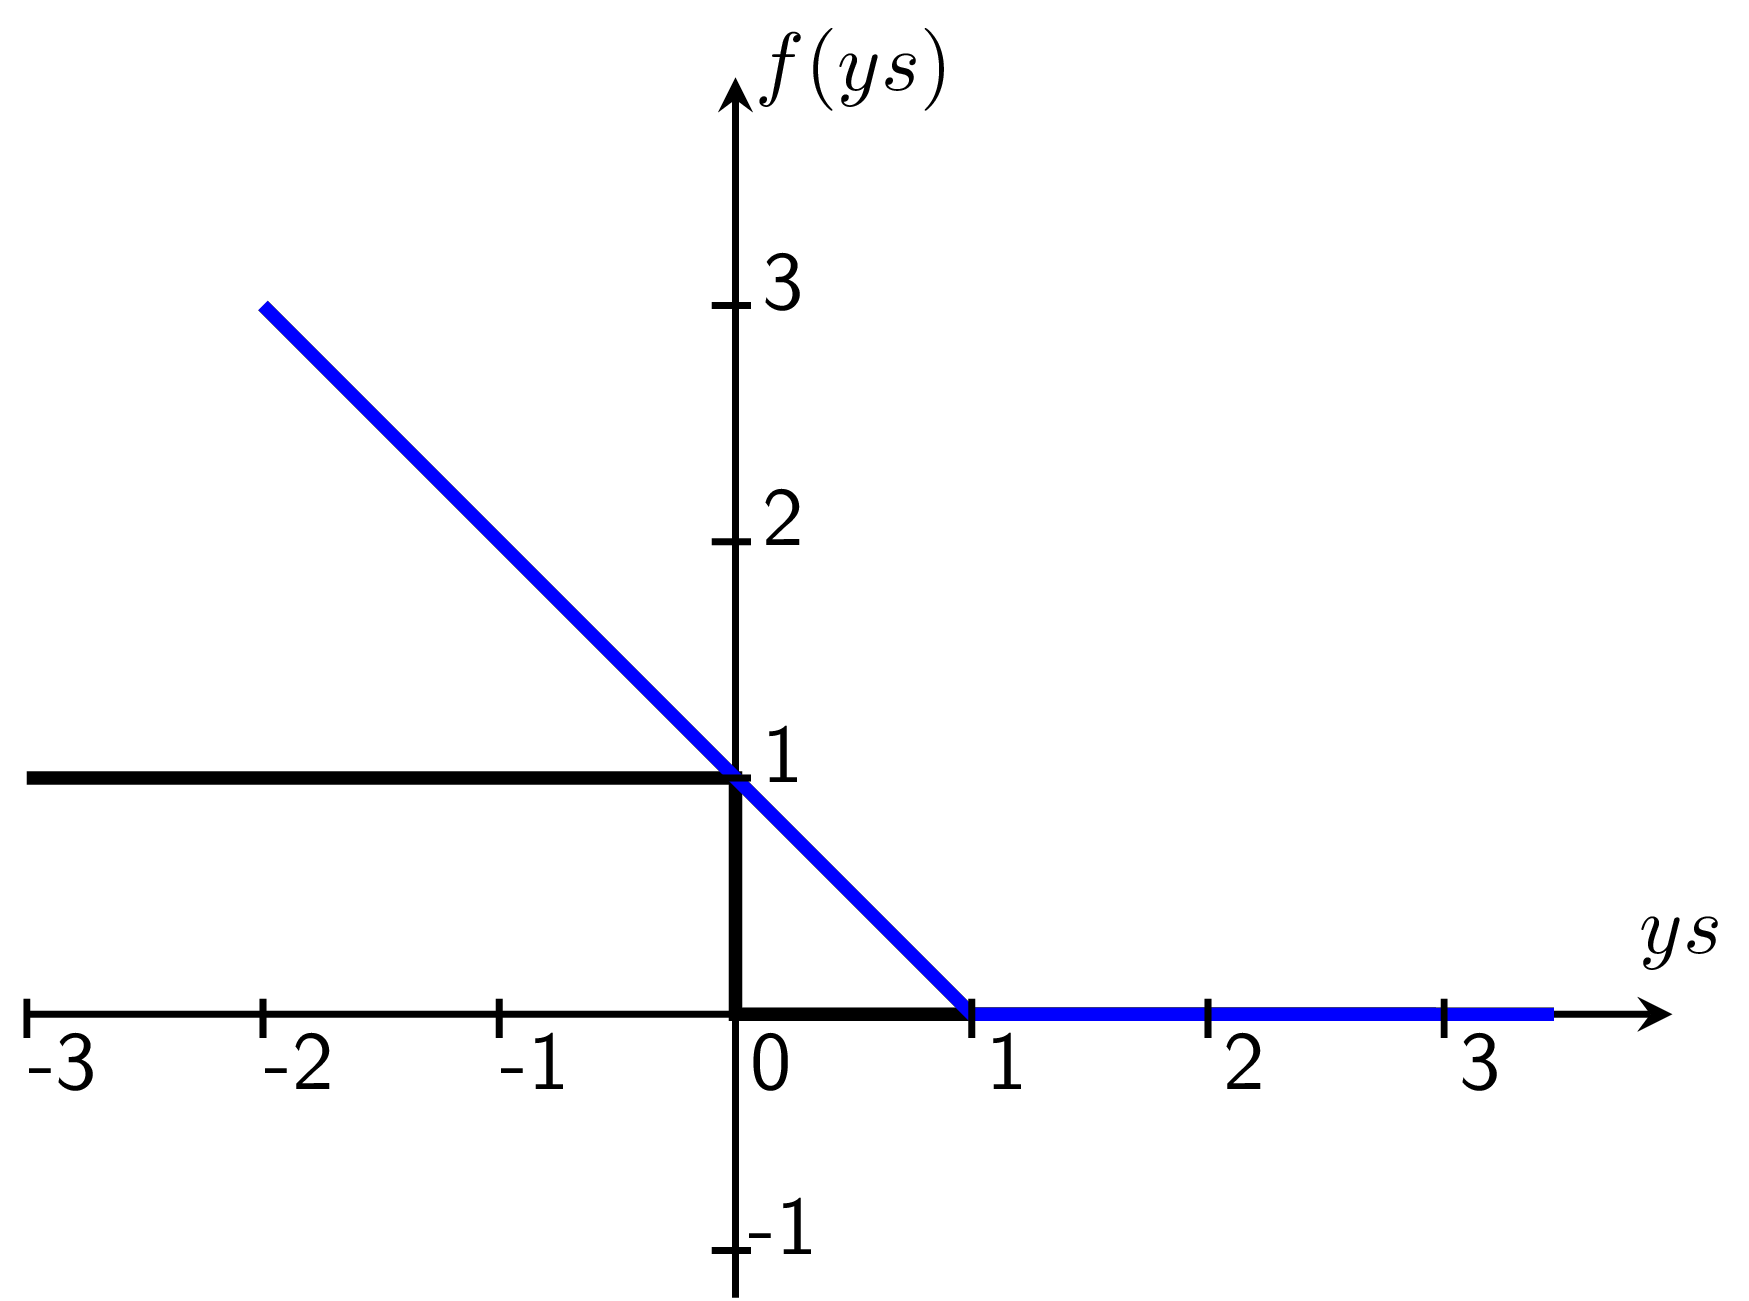
\includegraphics[scale=0.08]{hinge.png}
    \end{center}
    \caption{Đồ thị hàm số Hinge Loss}
    \label{refhinh1}
    \end{figure}
\end{center}
Với mỗi cặp $(w,b)$, đặt:
\begin{mybox}
$$ L_n(w,b) = max(0, 1- y_n(w^Tx_n + b)) $$
\end{mybox}
Lấy tổng tất cả các \textit{loss} này theo $n$ ta được: 
\begin{mybox}
$$ L(\mathbf{w}, b) = \sum_{n=1}^N L_i = \sum_{n=1}^N \max(0, 1 - y_n(\mathbf{w}^T\mathbf{x}_n + b)) $$ \end{mybox}
Với nhận xét nếu $(w,b)$ là nghiệm của bài toán thì $(aw,bw)$ cũng là nghiệm của bài toán với $a >1$. Do đó để nghiệm bài toán không trở nên lớn tuỳ ý do đó ta cần thêm số hạng \textit{regularization} để tránh \textit{overfit}. Sử dụng kỹ thuật \textit{weight decay} ta có thể thu được hàm mất mát của bài toán soft margin như sau: 
\begin{mybox}
$$ J(w,b) = \sum_{n=1}^N L_i = \sum_{n=1}^N \max(0, 1 - y_n(\mathbf{w}^T\mathbf{x}_n + b)) + \frac{\lambda}{2} ||w||^2_2 ~~~(2.19)$$ \end{mybox}
Bài toán này giống bài toán (2.18) với $\lambda = \frac{1}{C}$\\ \\
Đặt $\bar{x} = [x^T,1]^T$ và $\bar{w} = [w^T,b]^T$, bài toán (2.19) trở thành\\
\begin{mybox}
$$J(\mathbf{\bar{w}}) = \underbrace{\sum_{n=1}^N \max(0, 1 - y_n\bar{\mathbf{w}}^T\mathbf{\bar{x}}_n)}_{\text{hinge loss}} + \underbrace{\frac{\lambda}{2} ||\mathbf{w}||_2^2}_{\text{regularization}} $$ \end{mybox}
\subsection{Tối ưu hàm mất mát}
Đặt: 
\begin{mybox}
$$ Z = [y_1 \mathbf{\bar{x}}_1, y_2 \mathbf{\bar{x}}_2, \dots, y_N\mathbf{\bar{x}}_N] $$
$$ u = [y_1\mathbf{\bar{w}}^T\mathbf{\bar{x}}_1,y_2\mathbf{\bar{w}}^T\mathbf{\bar{x}}_2, \dots, y_N \mathbf{\bar{w}}^T \mathbf{\bar{x}}_N] = \mathbf{\bar{w}}^T\mathbf{Z}   $$


\end{mybox}
Đặt $\mathcal{H} = \{n: u_n < 1\}$. Lấy đạo hàm theo $\bar{w}$, ta có:
\begin{mybox}
$$\nabla J(\mathbf{\bar{w}}) = \sum_{n \in \mathcal{H}} - y_n\mathbf{\bar{x}}_n  + \lambda 
\left[\begin{matrix}
\mathbf{w}\\
0
\end{matrix}\right]$$ \end{mybox}
Quy tắc cập nhật của $\bar{w}$ sẽ là: 
\begin{mybox}
$$ \mathbf{\bar{w}} = \mathbf{\bar{w}} - \eta \left(\sum_{n \in \mathcal{H}} - y_n\mathbf{\bar{x}}_n  + \lambda \left[\begin{matrix}
\mathbf{w}\\
0
\end{matrix}\right]\right) $$ \end{mybox}
\subsection{Minh họa nghiệm tìm được}
\begin{figure}[H]
     \centering
     \begin{subfigure}[H]{0.3\textwidth}
         \centering
         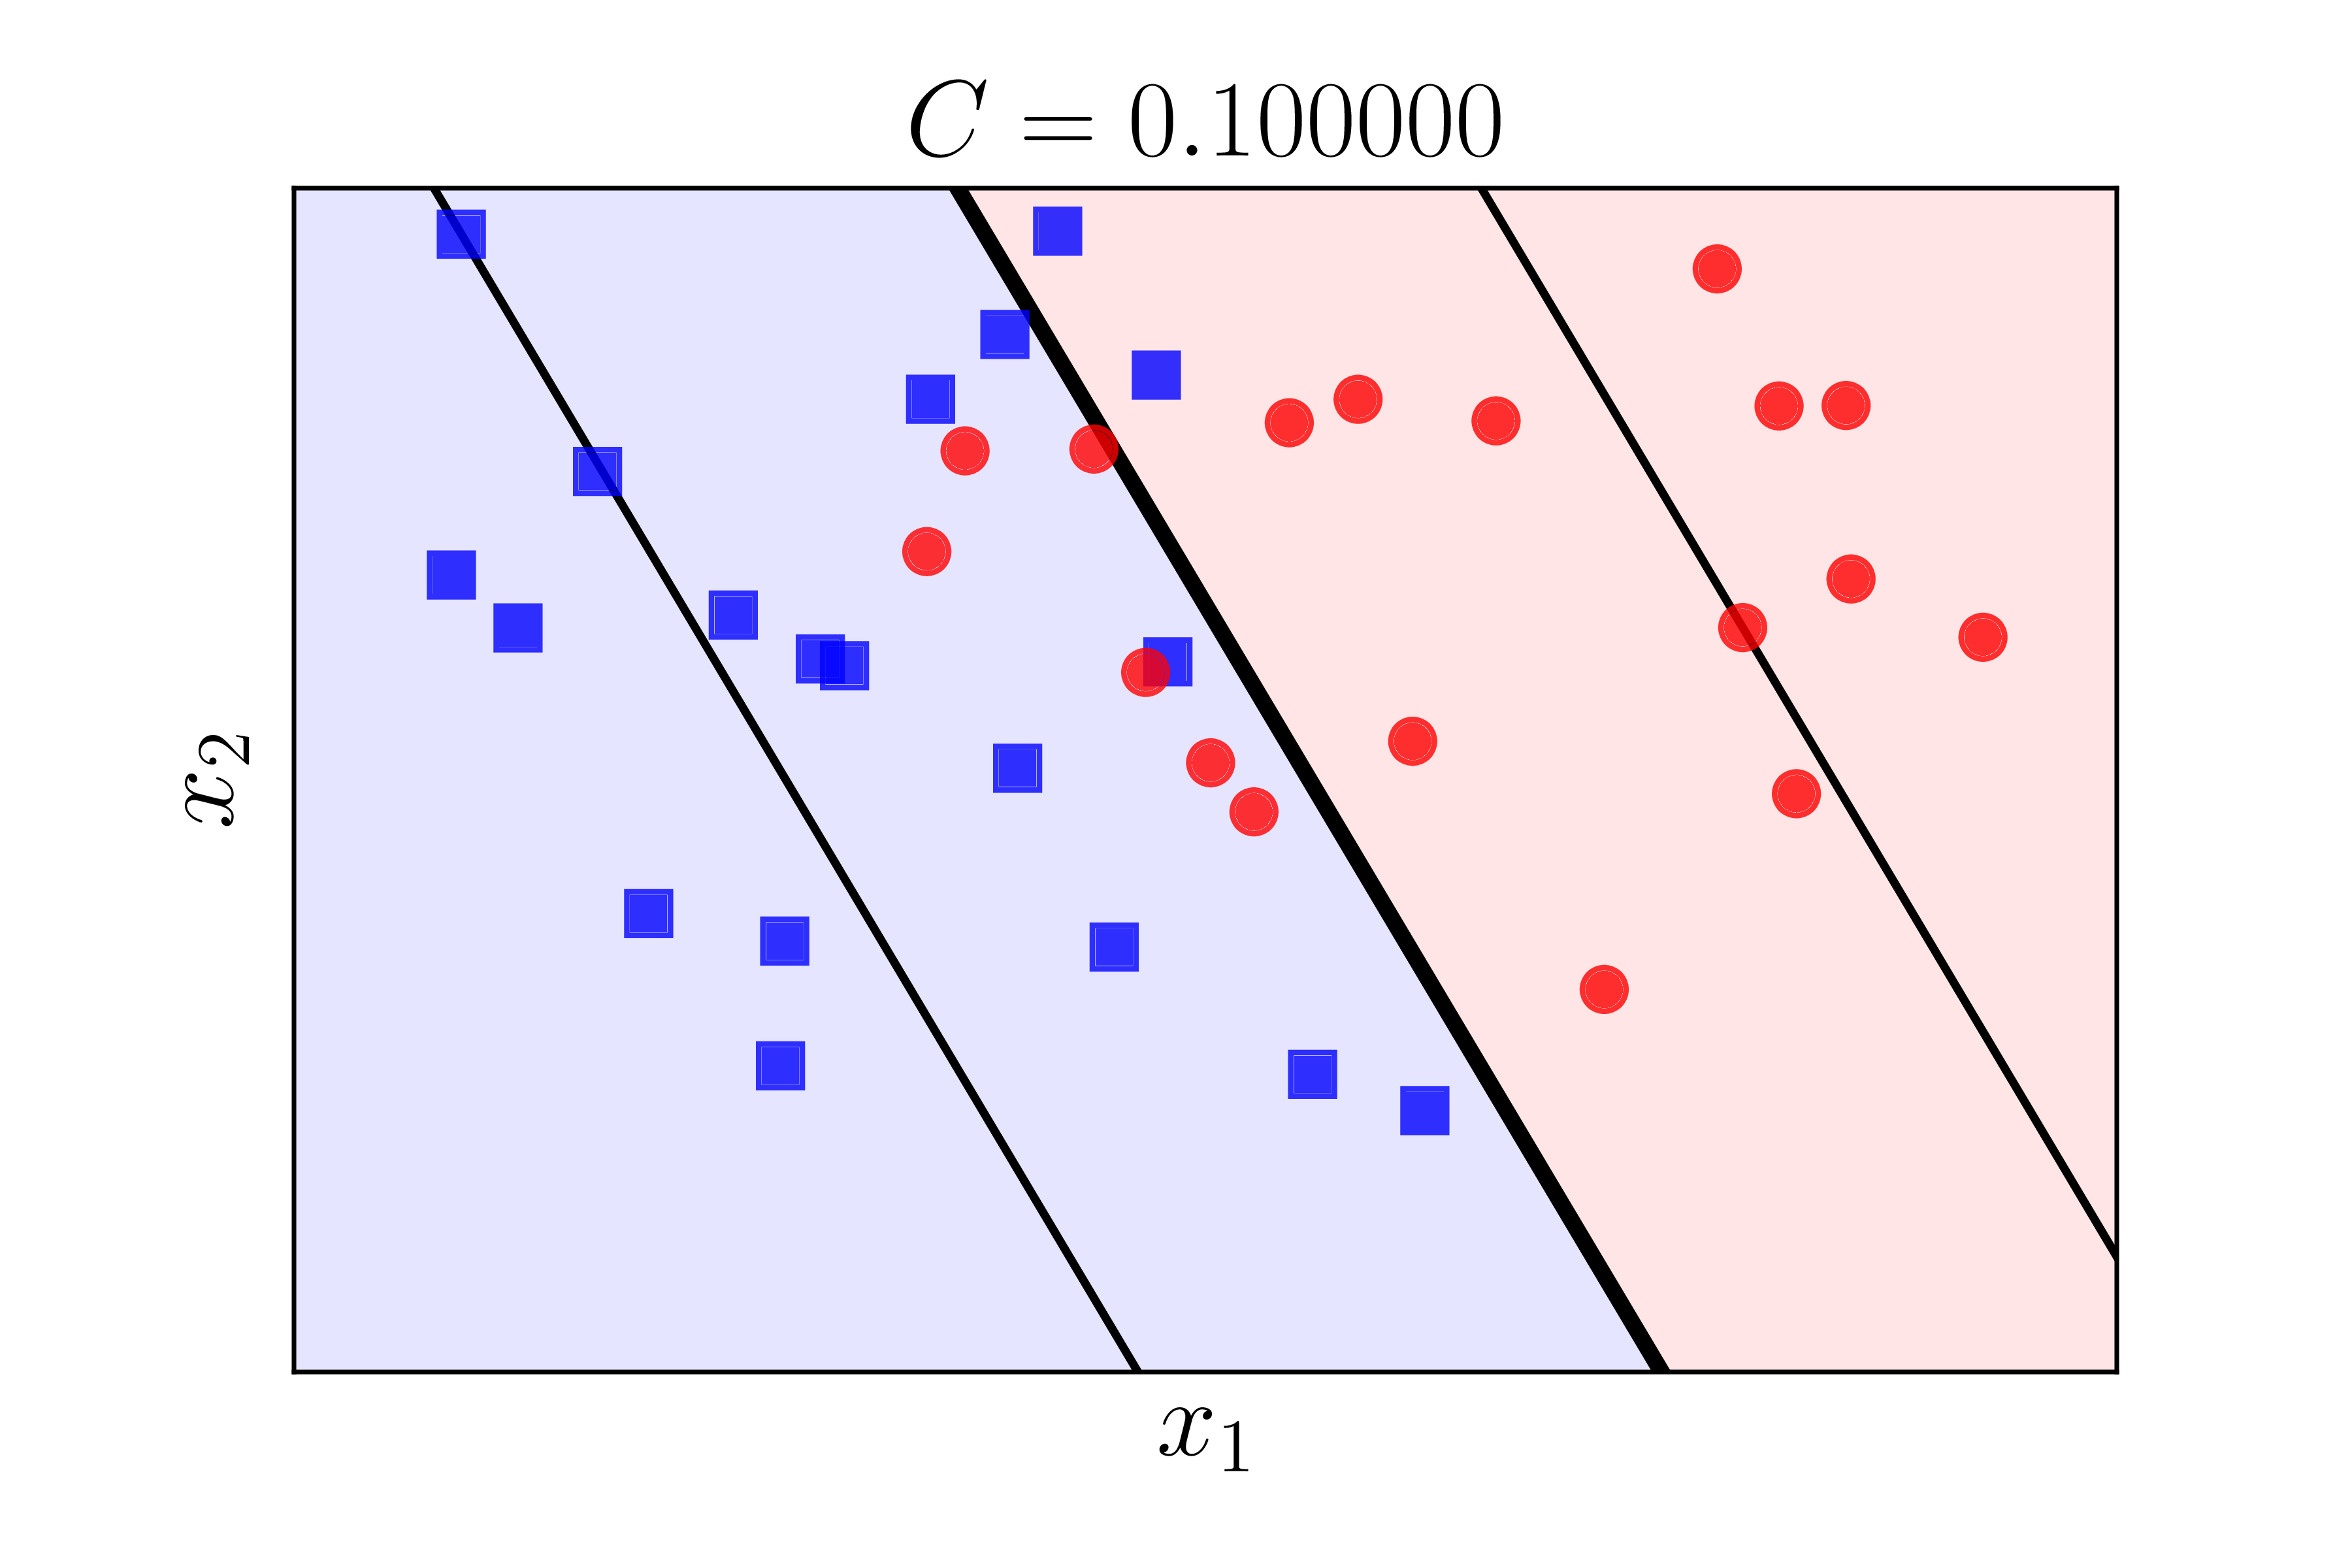
\includegraphics[width=\textwidth]{ssvm5_01.png}
         \caption{Minh họa nghiệm tìm được theo C = 0.1}
         \label{refhinh1}
     \end{subfigure}
     \hfill
     \begin{subfigure}[H]{0.3\textwidth}
         \centering
         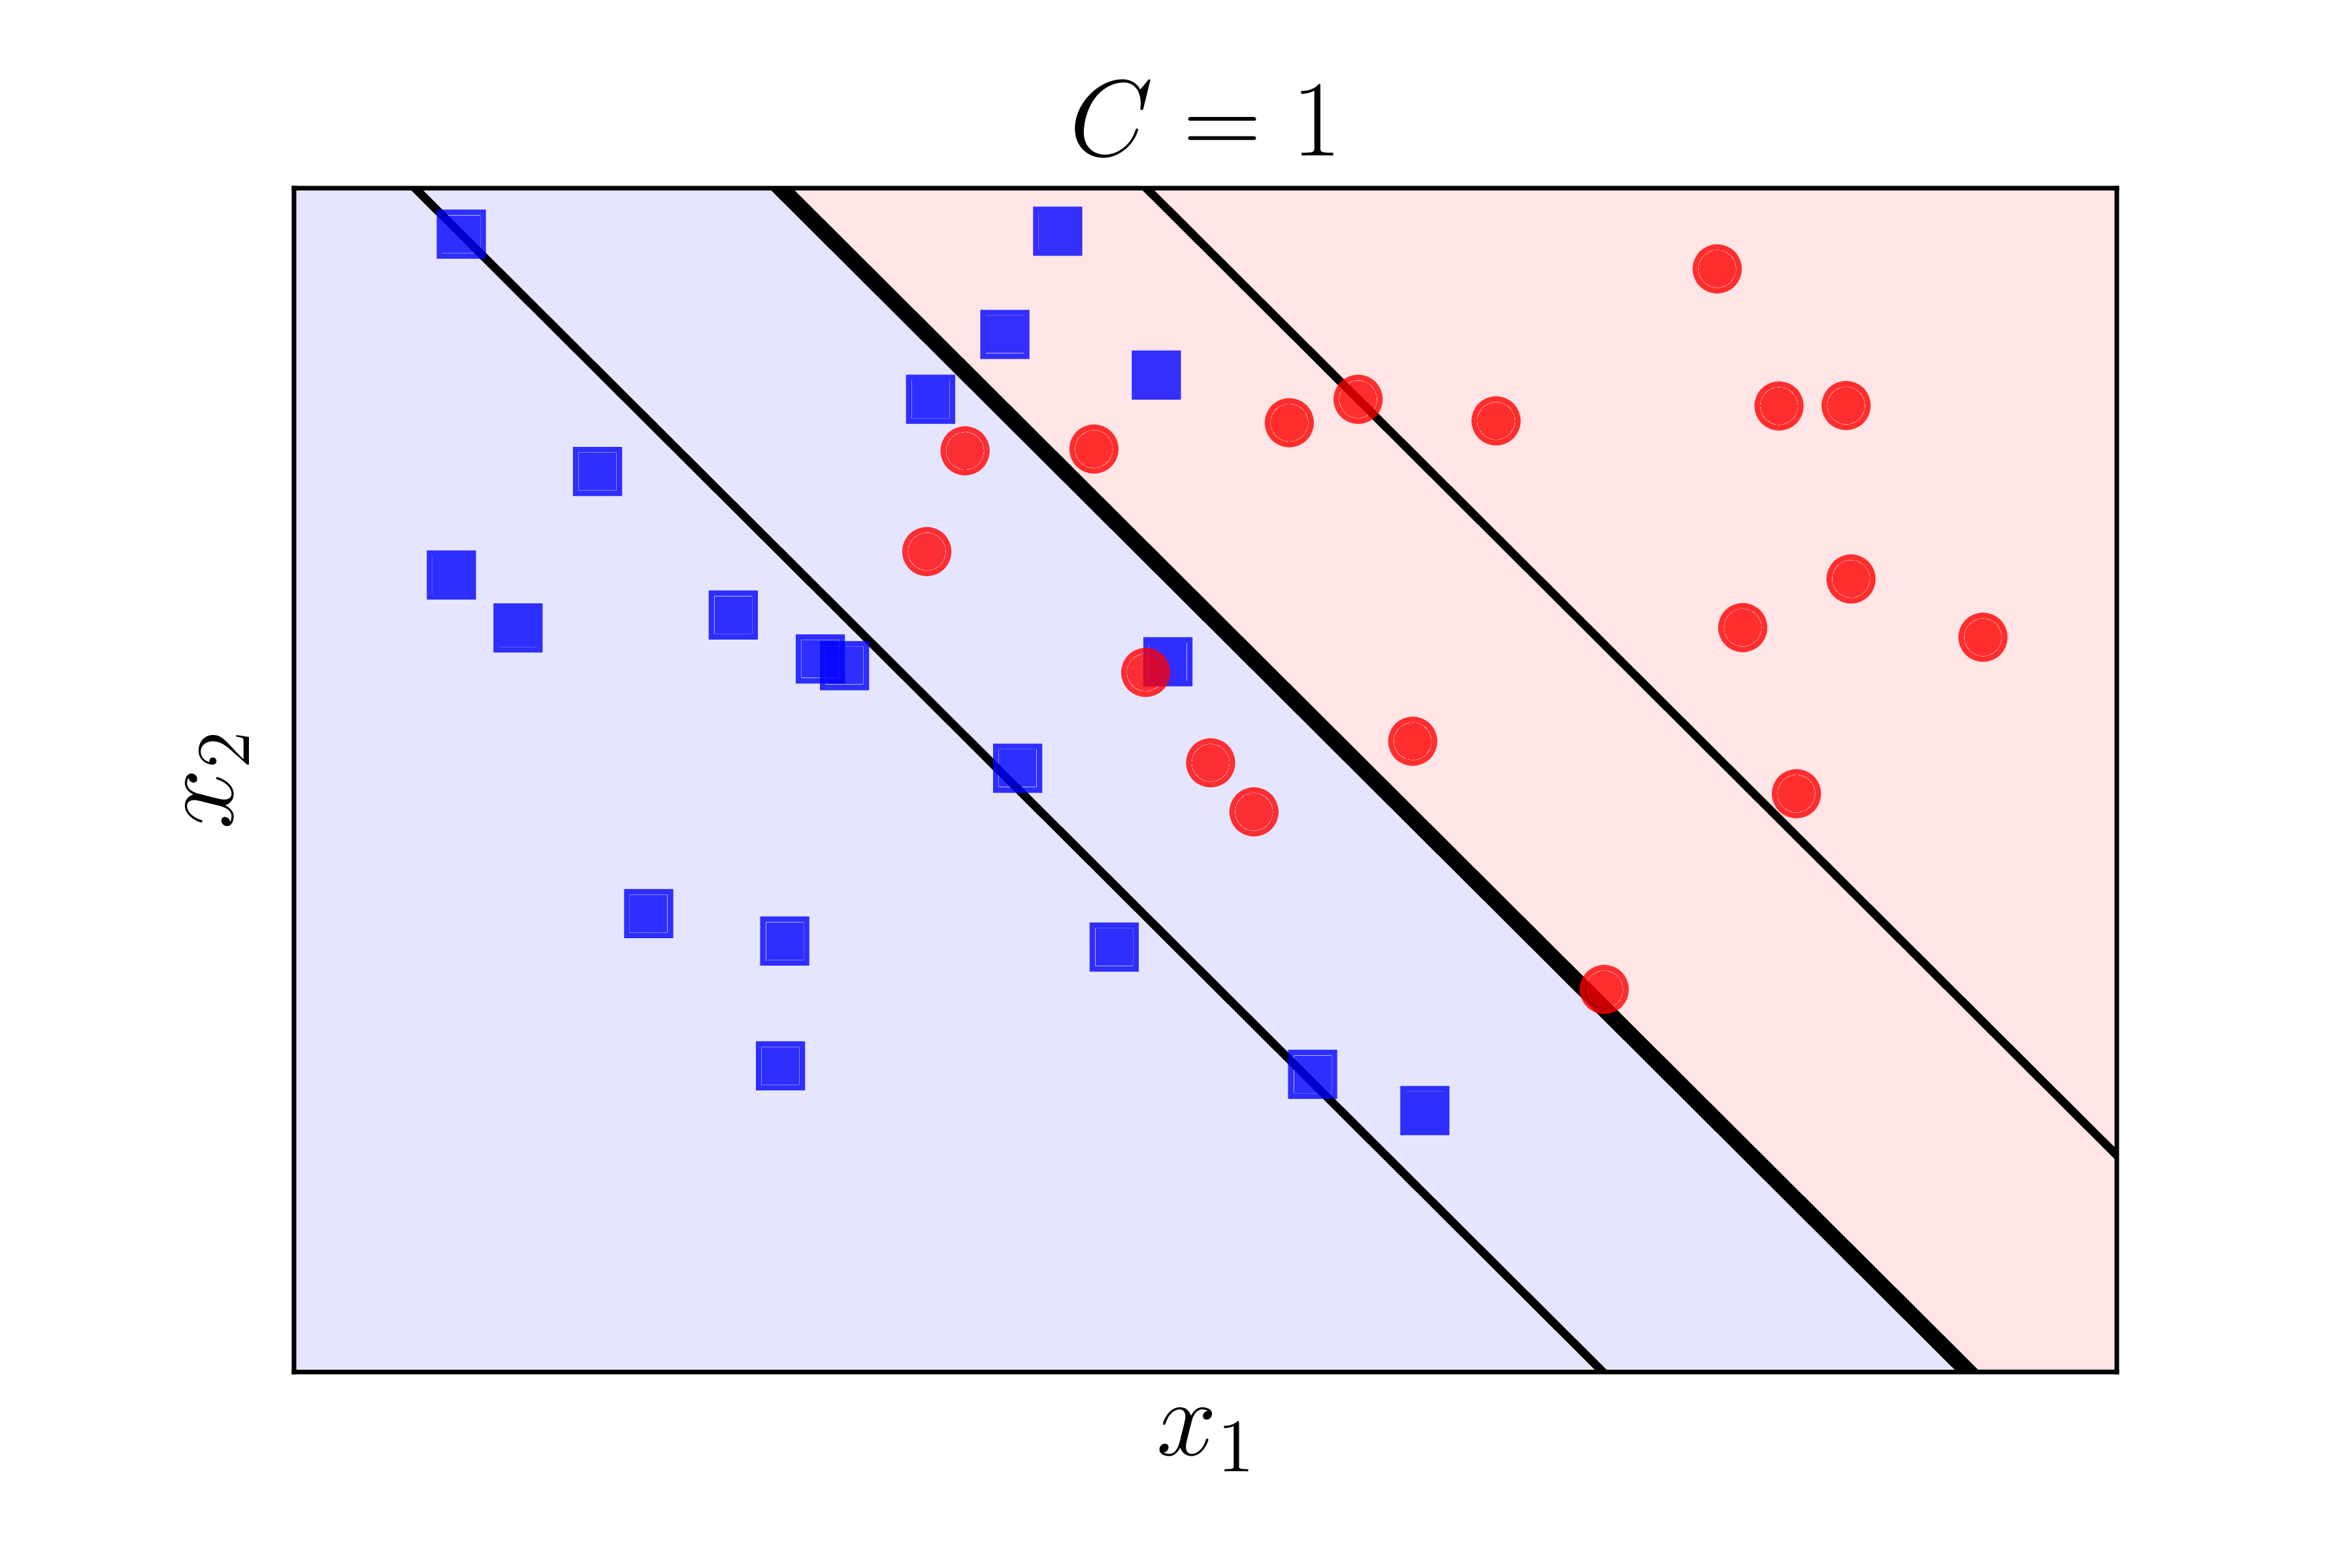
\includegraphics[width=\textwidth]{ssvm5_1.png}
         \caption{Minh họa nghiệm tìm được theo C = 1}
         \label{refhinh1}
     \end{subfigure}
     \hfill
     \begin{subfigure}[H]{0.3\textwidth}
         \centering
         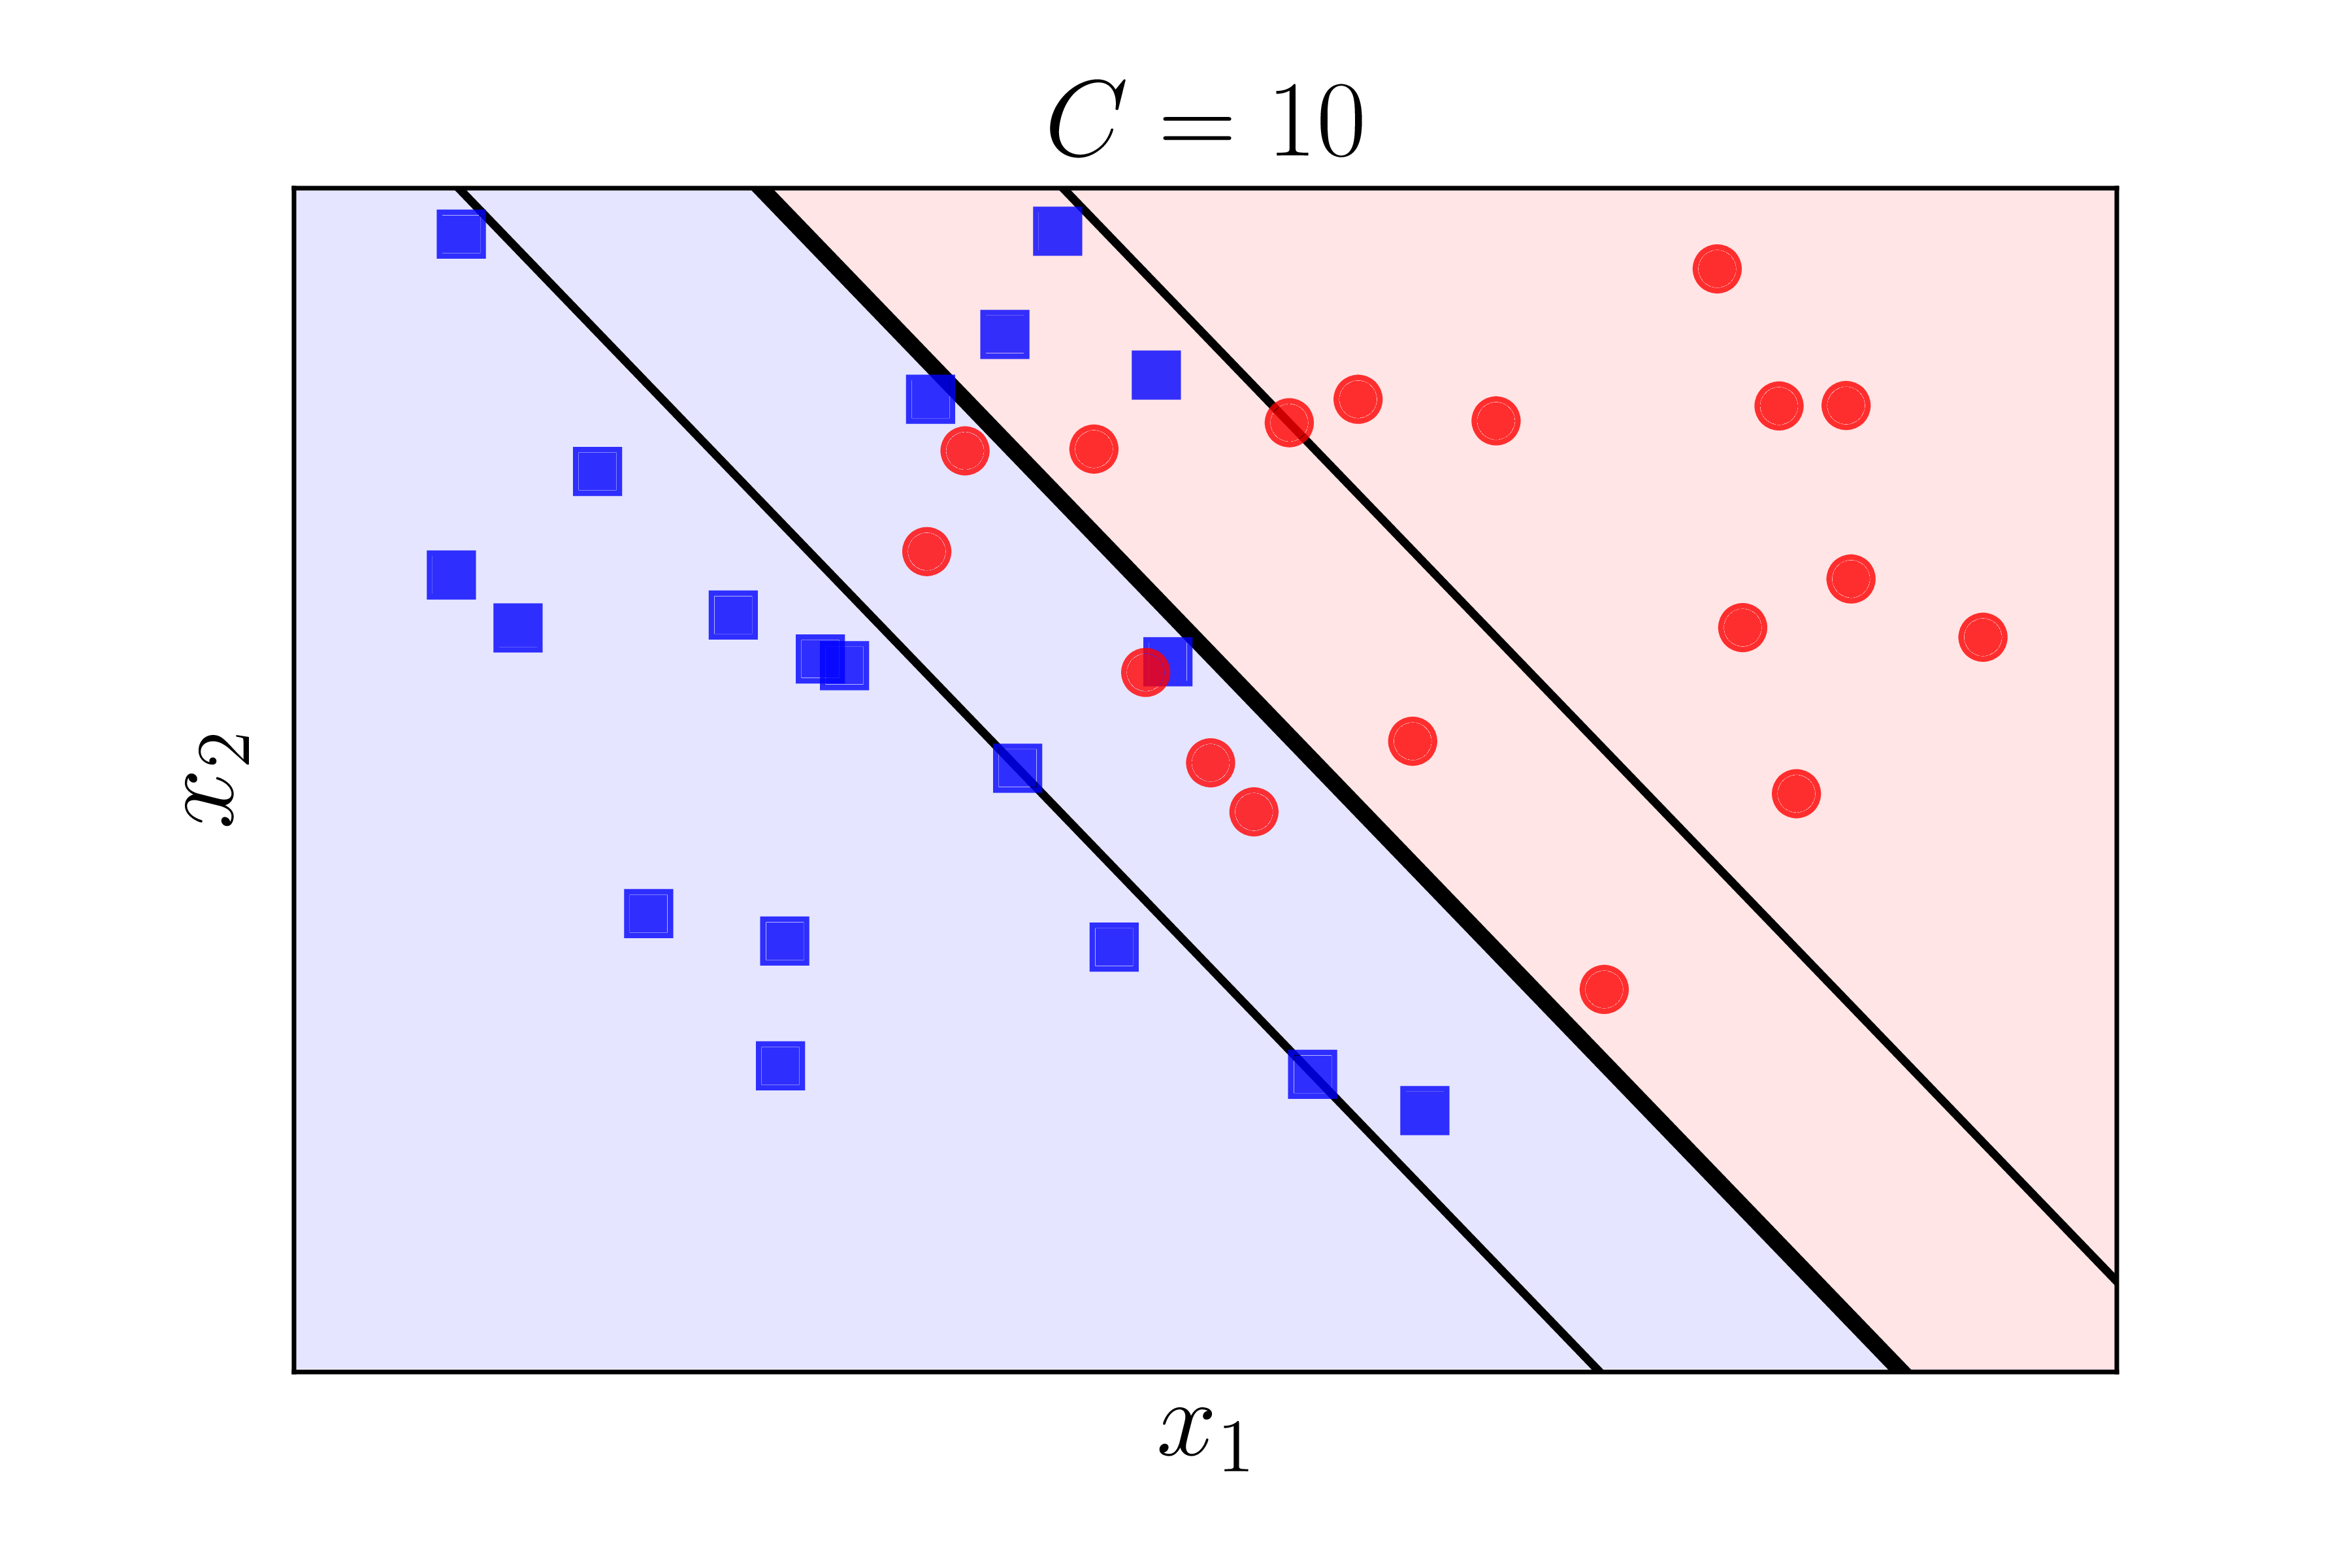
\includegraphics[width=\textwidth]{ssvm5_10.png}
         \caption{Minh họa nghiệm tìm được theo C = 10}
         \label{refhinh1}
     \end{subfigure}
     \hfill
     \begin{subfigure}[H]{0.3\textwidth}
         \centering
         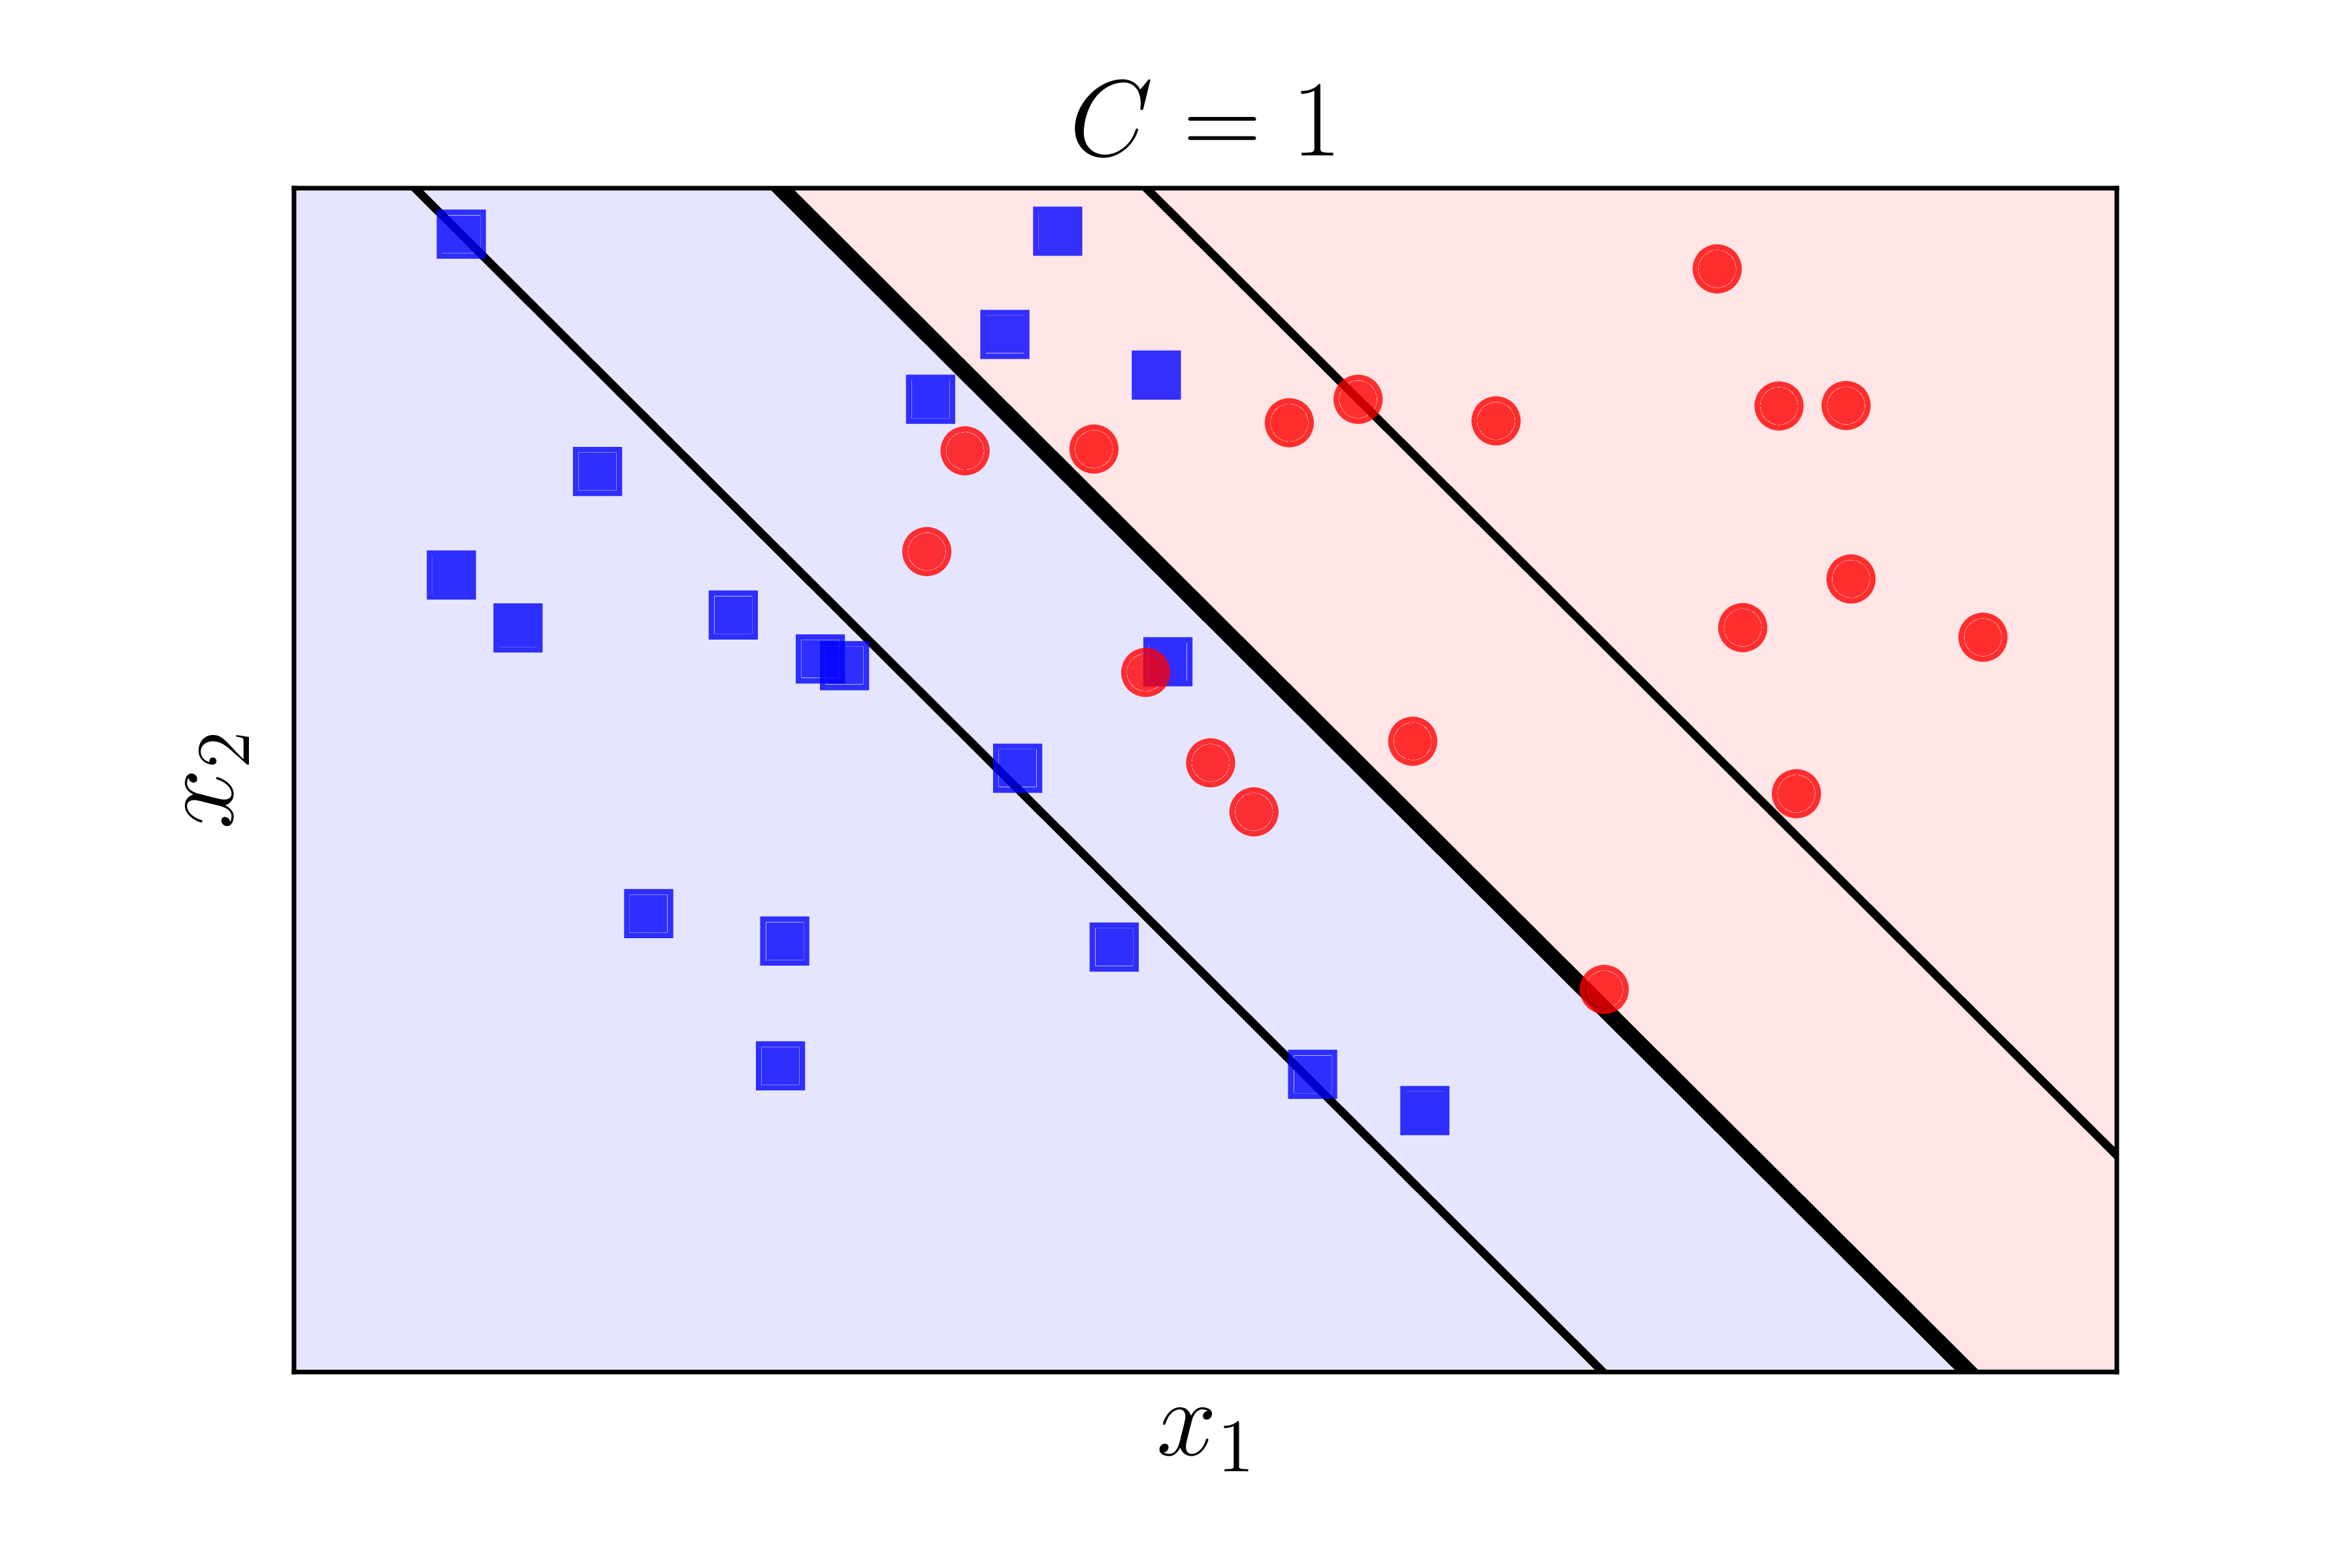
\includegraphics[width=\textwidth]{ssvm5_1.png}
         \caption{Minh họa nghiệm tìm được theo C = 100}
         \label{refhinh1}
     \end{subfigure}
     \hfill
        \caption{Minh họa nghiệm tìm được theo C}
        \label{fig:three graphs}
\end{figure}
\subsection{Giải bài toán SVM bằng thư viện scikit-learn của python} 
\subsubsection{Thư viện scikit-learn}
Scikit-learn (Sklearn) là thư viện mạnh mẽ dành cho các thuật toán học máy được viết trên ngôn ngữ Python. Thư viện cung cấp một tập các công cụ xử lý các bài toán học máy và các mô hình thống kê gồm: phân lớp, hồi quy, gom cụm, và thu giảm số chiều.
\subsubsection{Giải bài toán SVM bằng thư viện scikit-learn}
Bài toán SVM được hỗ trợ trong thư viện và được được thư viện cung cấp các hàm hỗ trợ
\begin{lstlisting}
from sklearn.svm import SVC
y1 = y.reshape((2*N,))
X1 = X.T # each sample is one row
clf = SVC(kernel = 'linear', C = 1e5) # just a big number 

clf.fit(X1, y1) 

w = clf.coef_
b = clf.intercept_
print('w = ', w)
print('b = ', b)
\end{lstlisting}
Trong đó $X$ và $y$ lần lượt là tập dữ liệu và nhãn có dữ liệu ma trận và vector.\\
$y1$ là dữ liệu được làm phẳng (đưa về mảng 1 chiều) của $y$.\\
$X1$ là ma trận $X$ chuyển vị.\\
SVC là một lớp trong thư viện sk-learn được khởi tạo với những thông số ban đầu như tên kernel, hằng số $C$.\\
Hàm \textit{fit} là một hàm thuộc tính của lớp SVC để huấn luyện dữ liệu. 
Hai thuộc tính \textit{w} và \textit{b} là nghiệm của bài toán sau khi huấn luyện \\



\section{Sử dụng \textit{kernel} trong bài toán SVM khi dữ liệu không khả phân tách tuyến tính}
\subsection{Sự tương đồng của các lớp bài toán trong SVM}
Các bài toán phân lớp trong lĩnh vực học máy thường được tiếp cận từ dễ đến khó, bắt đầu từ các bài toán khả phân tách tuyến tính, đến các bài toán gần như phân tách tuyến tính. Khó hơn là các bài toán phân lớp nhiều lớp.
\begin{table}
\begin{tabular}{|l|l|l|}
\hline 
Neural Networks & Support Vector Machine & Tính chất chung\\ 
\hline 
PLA & Hard Margin SVM & Khả phân tách tuyến tính\\ 
\hline 

Logistic Regression & Soft Margin SVM & Gần khả phân tách tuyến tính\\ 
\hline 
Multi-layer Perceptron & 	Kernel SVM & Dữ liệu không linearly separable\\ 
\hline
\end{tabular}
\caption{So sánh bài toán SVM và bài toán neural network}
\label{bang 2.1}
\end{table}
\subsection{Kernel SVM}
Ý tưởng cơ bản của kernel SVM và các phương pháp kernel nói chung là tìm một phép biến đổi sao cho dữ liệu ban đầu là không phân biệt tuyến tính được biến sang không gian mới. Ở không gian mới này, dữ liệu trở nên phân biệt tuyến tính.
Nói một cách ngắn gọn, kernel SVM là việc đi tìm một hàm số biến đổi dữ liệu x từ không gian ban đầu thành dữ liệu trong một không gian mới bằng hàm số $\Phi(x)$. Trong ví dụ này, hàm $\Phi$ đơn giản là giới thiệu thêm một chiều dữ liệu mới (một đặc trưng mới) là một hàm số của các đặc trưng (features) đã biết. Hàm số này cần thỏa mãn mục đích của chúng ta: Trong không gian mới, dữ liệu giữa hai lớp là phân biệt tuyến tính hoặc gần như phần biệt tuyến tính. Khi đó, ta có thể dùng các bộ phân lớp tuyến tính thông thường như PLA, Logistic Regression, hay Hard/Soft Margin SVM.
\subsubsection{Tính chất của các hàm kernel}
Các hàm kernel cần có các tính chất sau:
\begin{itemize}
    \item Đối xứng
    \item Điều kiện Mercer:
    \begin{mybox}
    $$\sum_{n=1}^N \sum_{m=1}^N k(\mathbf{x}_m, \mathbf{x}_n) c_nc_m \geq 0, ~~ \forall c_i \in \mathbb{R}, i = 1, 2, \dots, N $$ 
    \end{mybox}
    
\end{itemize}
\subsection {Một số hàm kernel thông dụng}
\subsubsection{Linear}
Đây là kernel tích vô hướng giữa hai vector được định nghĩa bằng công thức: \\

\begin{mybox}
$$k(\mathbf{x}, \mathbf{z}) = \mathbf{x}^T\mathbf{z}$$ 
\end{mybox}
\subsubsection{Polynomial}
\begin{mybox}
$$k(\mathbf{x}, \mathbf{z}) = (r + \gamma \mathbf{x}^T\mathbf{z})^d$$
\end{mybox}
Với $d$ là một số dương để chỉ bậc của đa thức. $d$ có thể không là số tự nhiên vì mục đích chính của ta không phải là bậc của đa thức mà là cách tính kernel. Polynomial kernel có thể dùng để mô tả hầu hết các đa thức có bậc không vượt quá $d$ nếu $d$ là một số tự nhiên.
\begin{center}
    \begin{figure}[H]
    \begin{center}
     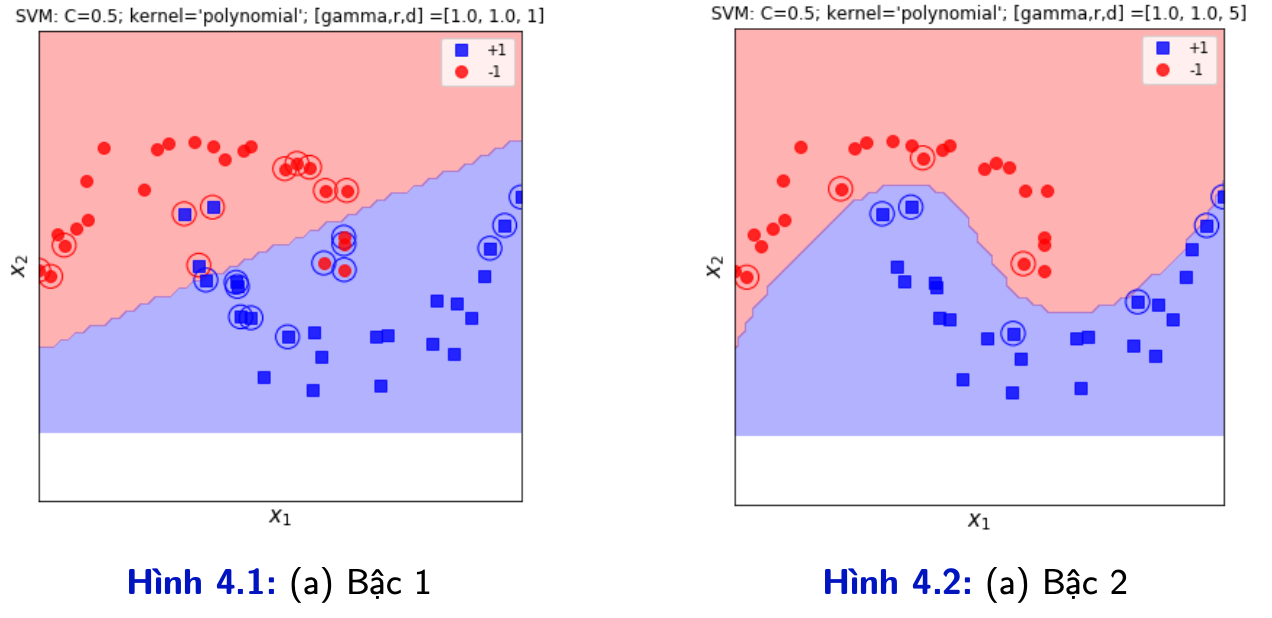
\includegraphics[scale=0.6]{poly12.png}
    \end{center}
    \caption{Minh họa kernel polynomial theo d bậc thấp}
    \label{Hình 4.4}
    \end{figure}
\end{center}
\begin{center}
    \begin{figure}[H]
    \begin{center}
     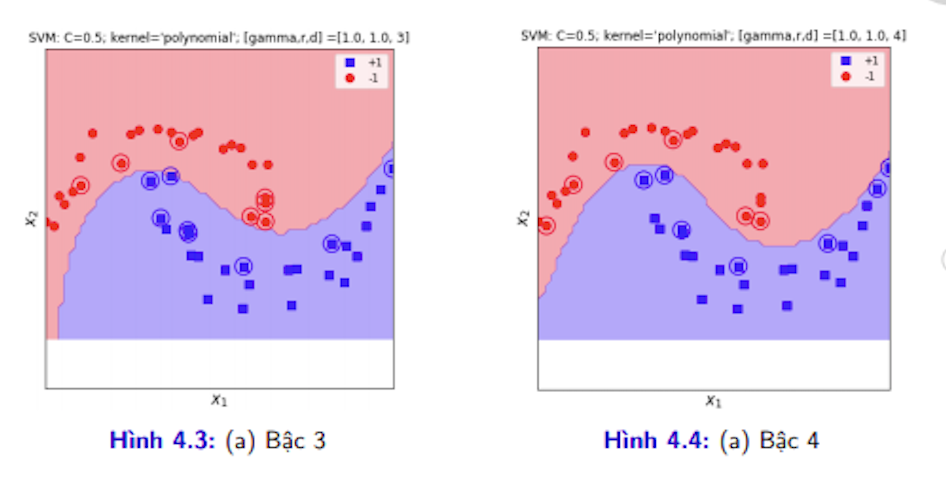
\includegraphics[scale=0.7]{poly1.png}
    \end{center}
    \caption{Minh họa kernel polynomial theo d bậc cao}
    \label{Hình 4.4}
    \end{figure}
\end{center}
\subsubsection{Radial Basic Function (RBF)}
Radial Basic Function (RBF) kernel hay Gaussian kernel được sử dụng nhiều nhất trong thực tế. Đây cũng là lựa chọn mặc định trong thư viện sklearn. 
\begin{mybox}
$$ k(\mathbf{x}, \mathbf{z}) = \exp(-\gamma ||\mathbf{x} - \mathbf{z}||_2^2), ~~ \gamma > 0 $$ \end{mybox}
\begin{center}
    \begin{figure}[H]
    \begin{center}
     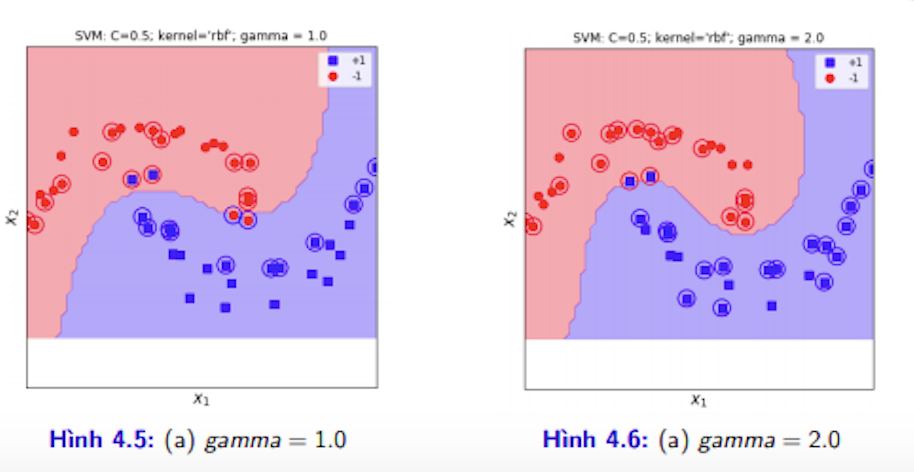
\includegraphics[scale=0.7]{poly.png}
    \end{center}
    \caption{Minh họa kernel rbf}
    \label{Hình 4.4}
    \end{figure}
\end{center}
\subsubsection{Sigmoid}
Sigmoid function cũng được sử dụng làm kernel:
\begin{mybox}
$$k(\mathbf{x}, \mathbf{z}) = \text{tanh}(\gamma \mathbf{x}^T\mathbf{z} + r)$$
\end{mybox}
\subsection{Tóm tắt các kernel thông dụng và cách sử dụng trong sklearn}

\begin{table}[H]
\begin{center}
\begin{tabular}{|l|l|l|}
\hline
Tên & Công thức & Kernel \\
\hline 
linear & $\mathbf{x}^T\mathbf{z}$ & 'linear'\\ 
\hline 
polynomial & $(r + \gamma \mathbf{x}^T\mathbf{z})^d $& 'poly'\\ 
\hline 
rbf & $\exp(-\gamma ||\mathbf{x} - \mathbf{z}||_2^2)$& 'rbf'\\ 
\hline 
sigmoid & 	$\text{tanh}(\gamma \mathbf{x}^T\mathbf{z} + r)$ & 'sigmoid'\\ 
\hline
\end{tabular}
\end{center}
\caption{Tóm tắt các kernel thường dùng}
\label{bang 2.1}
\end{table}
Ví dụ minh họa về tập dữ liệu có đặc tính gần phân biệt được 2 lớp.
\begin{center}
    \begin{figure}[H]
    \begin{center}
     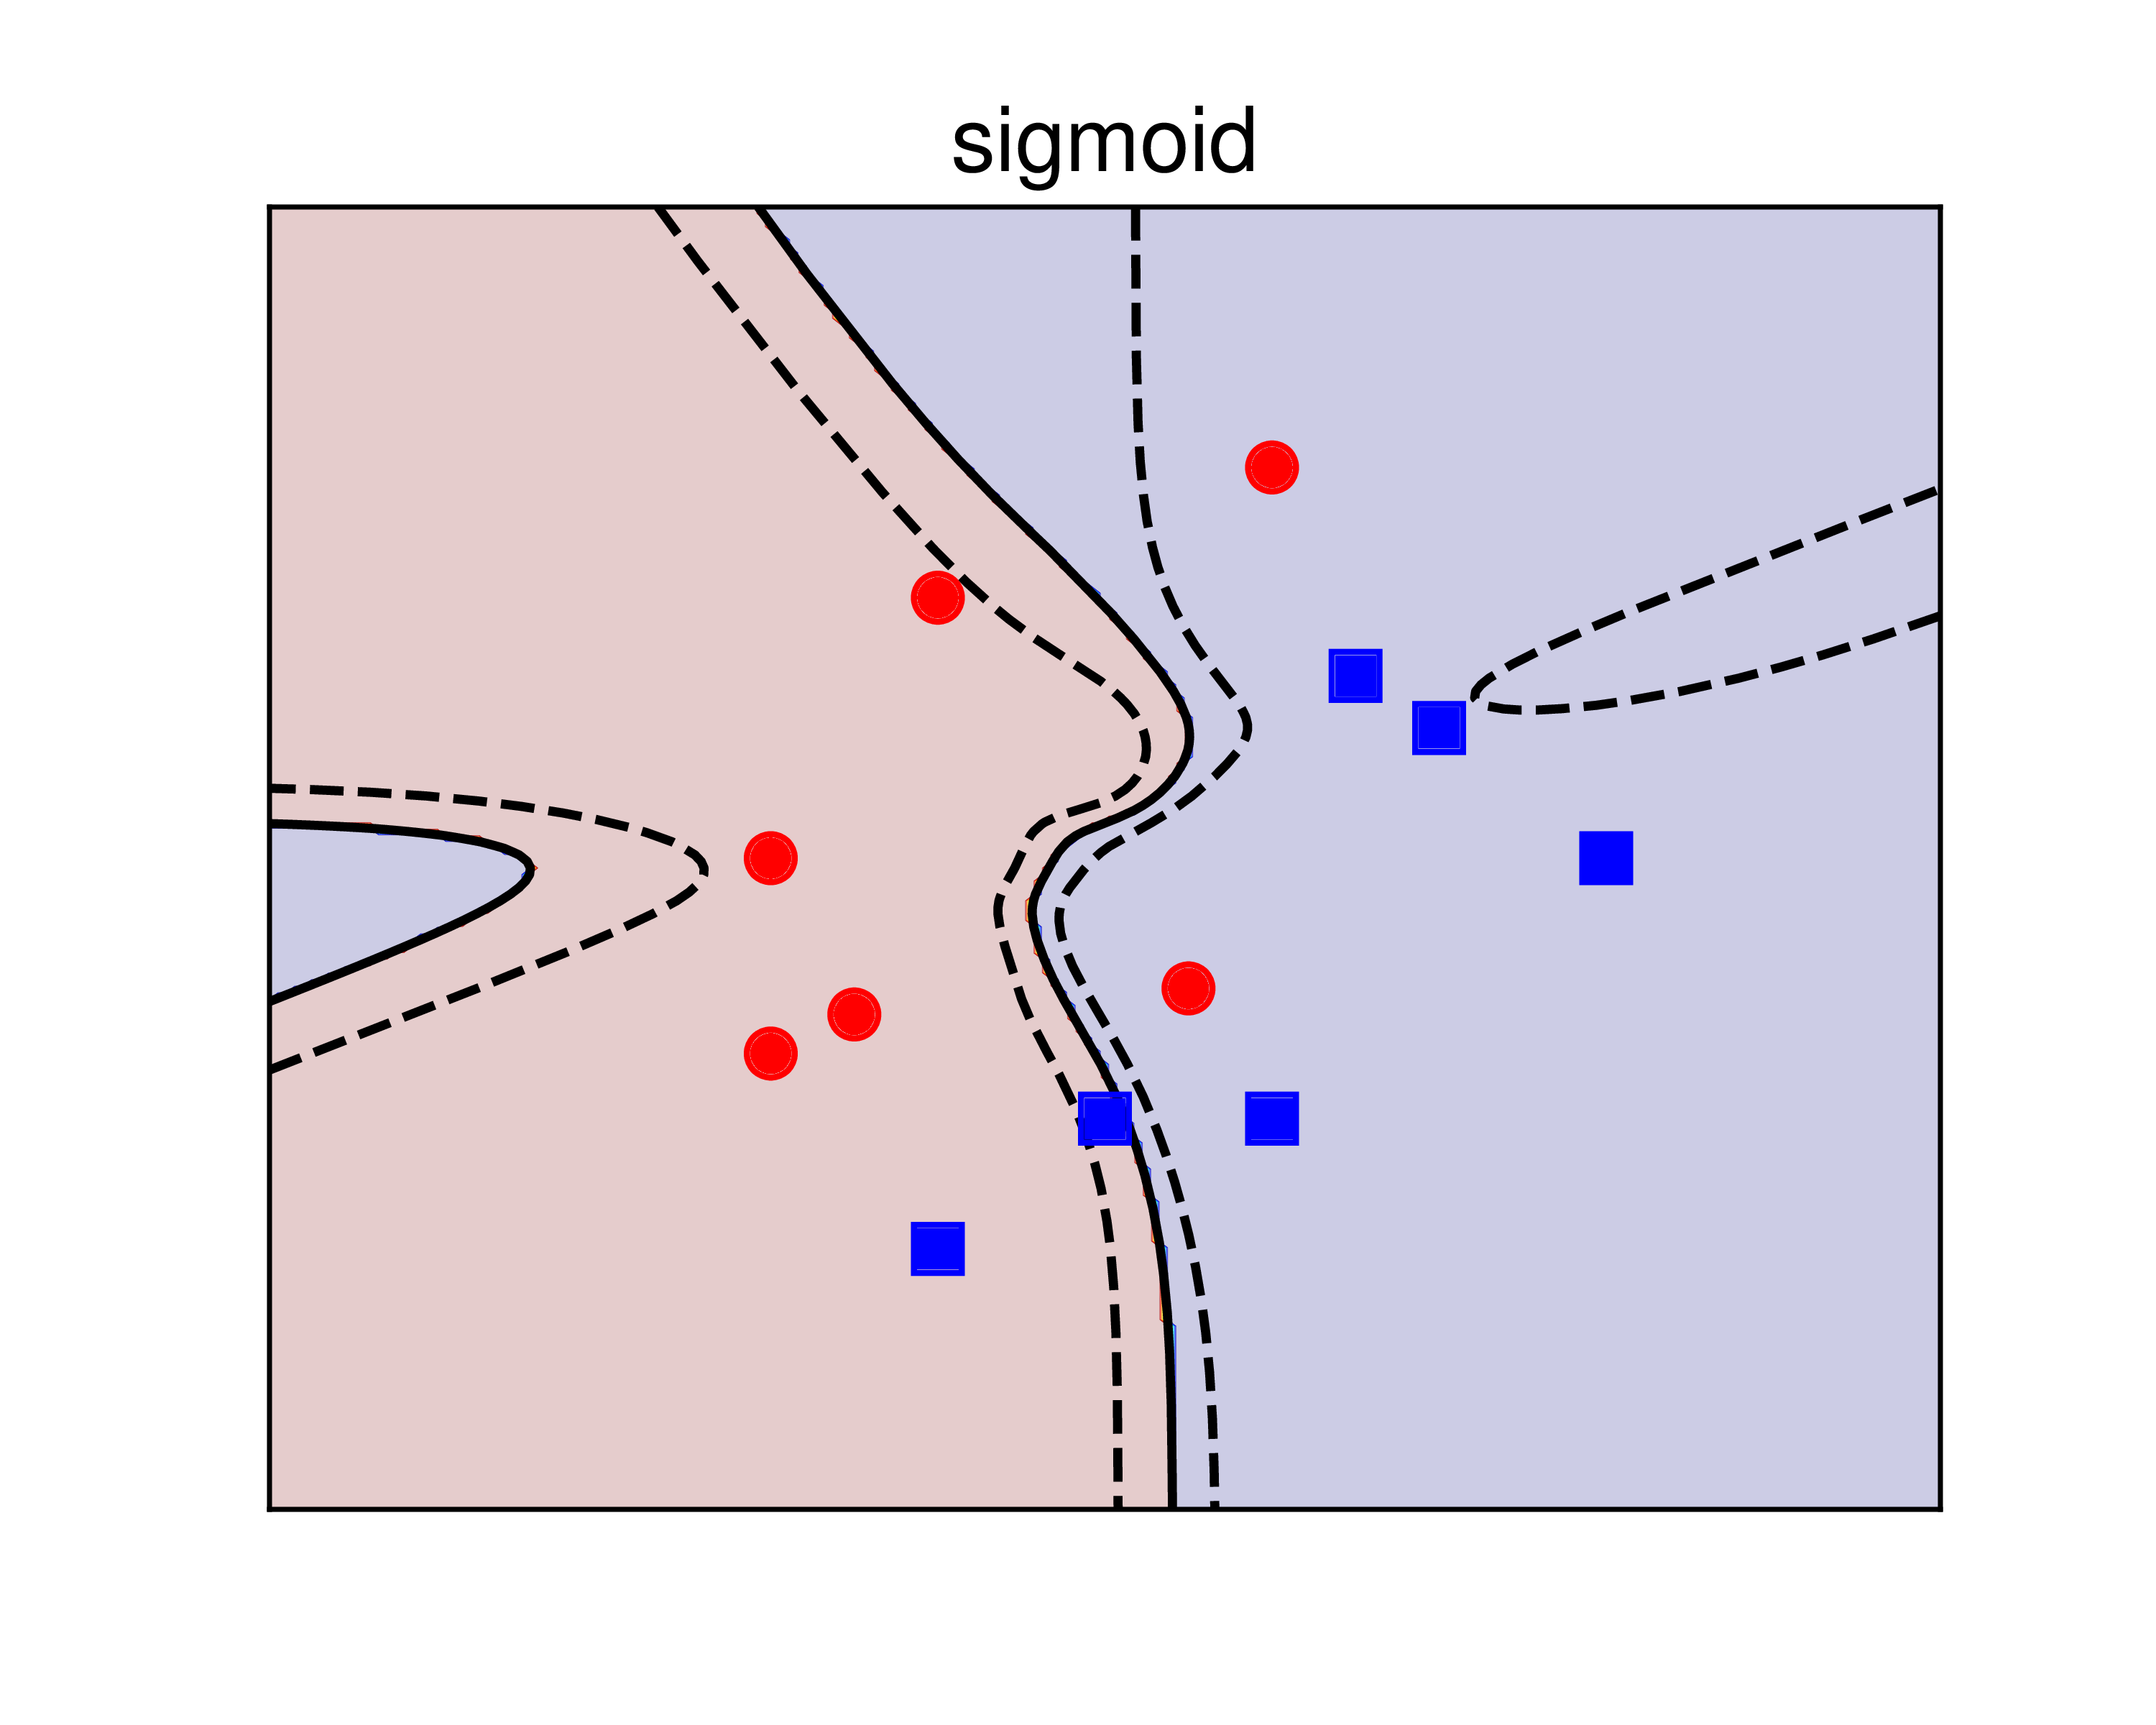
\includegraphics[scale=0.1]{kn1}
    \end{center}
    \caption{Minh họa signmoid kernel}
    \label{refhinh1}
    \end{figure}
\end{center}
\begin{center}
    \begin{figure}[H]
    \begin{center}
     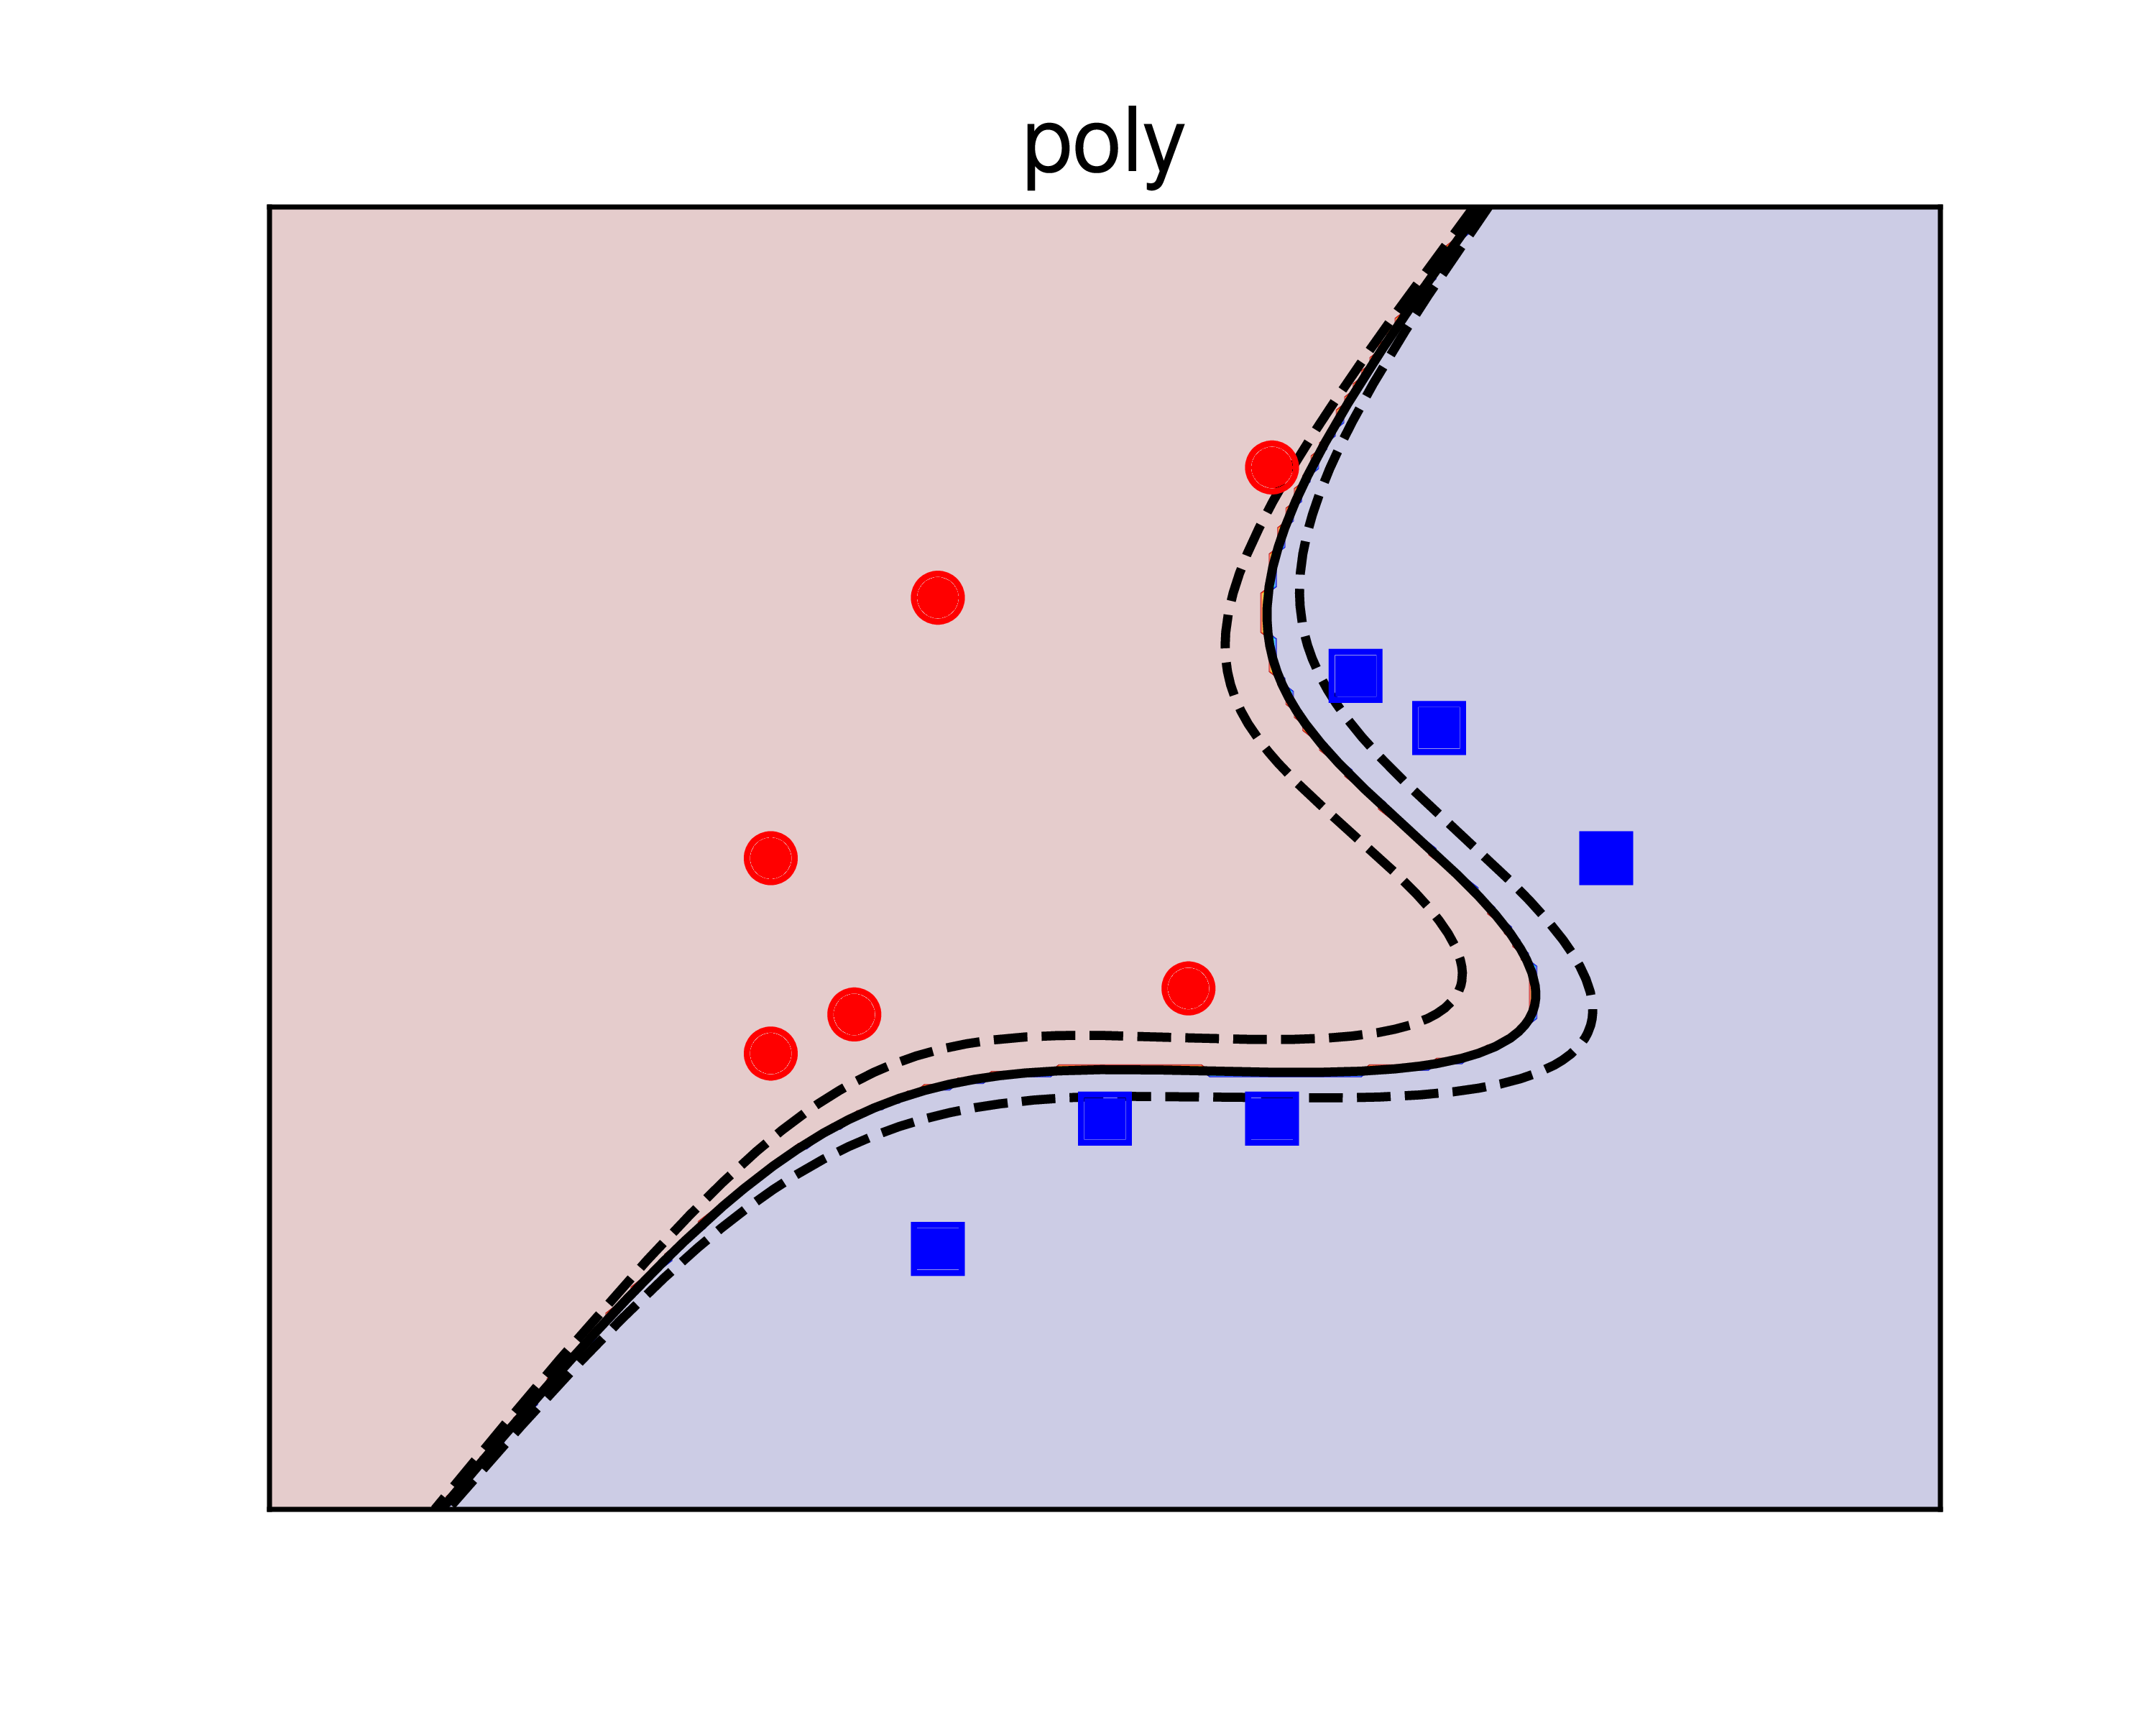
\includegraphics[scale=0.1]{kn2}
    \end{center}
    \caption{Minh hoạ polynomial kernel}
    \label{refhinh1}
    \end{figure}
\end{center}
\begin{center}
    \begin{figure}[H]
    \begin{center}
     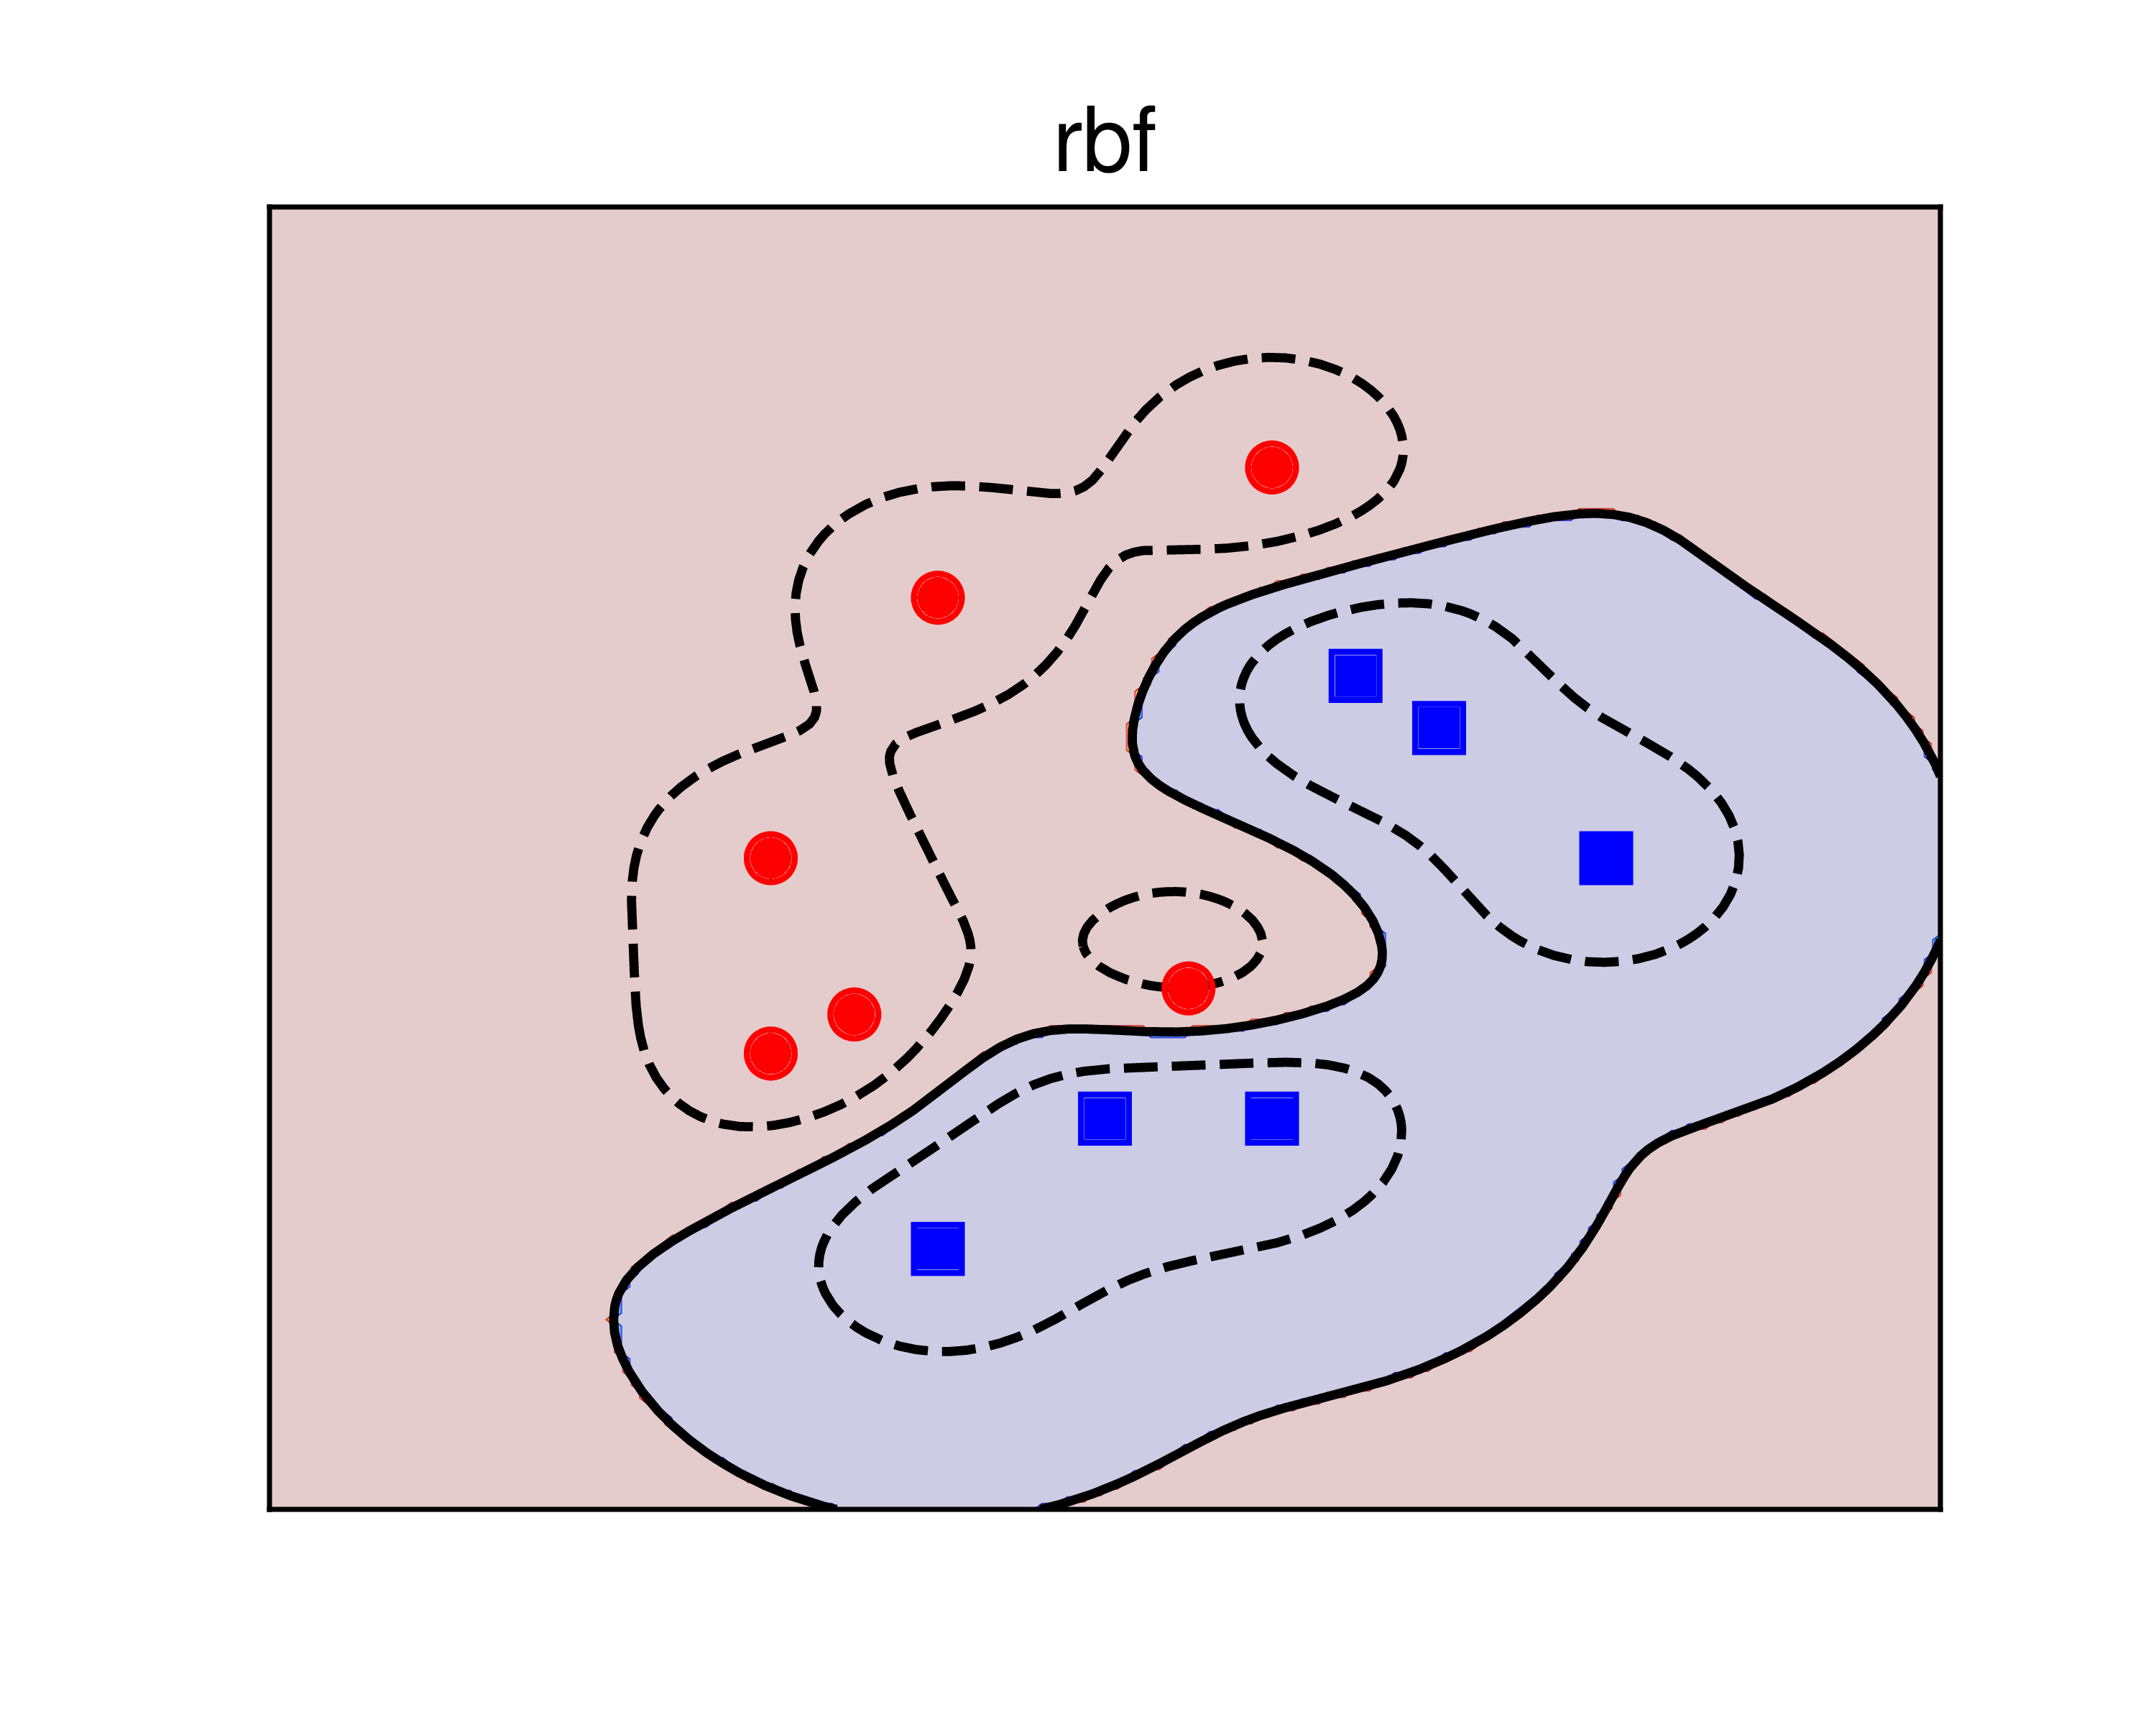
\includegraphics[scale=0.1]{kn3}
    \end{center}
    \caption{Minh họa rbf kernel}
    \label{refhinh1}
    \end{figure}
\end{center}
\subsection {Ưu điểm và nhược điểm của mô hình SVM }
Ưu điểm:
\begin{itemize}
    \item SVM là một công cụ tính toán hiệu quả trong không gian chiều cao.
    \item SVM hoạt động tốt ngay cả với các tập dữ liệu phi cấu trúc hoặc bán cấu trúc như văn bản, hình ảnh, âm thanh.
    \item SVM hoạt động tốt khi có sự phân tách rõ ràng giữa các lớp.
    \item SVM được sử dụng trong các bài toán hồi quy và phân loại.
    \item Thủ thuật kernel là sức mạnh thực sự của SVM. Với một hàm kernel thích hợp, chúng ta có thể giải quyết bất kỳ vấn đề phức tạp nào.
    \item Phân lớp thường là phi tuyến tính. Khả năng áp dụng Kernel mới cho phép linh động giữa các phương pháp tuyến tính và phi tuyến tính từ đó khiến cho hiệu suất phân loại lớn hơn.
    \item SVM có thể hoạt động tốt trong trường hợp số lượng các thuộc tính lớn hơn so với số lượng hàng dữ liệu của tập dữ liệu.
    \item Do chỉ có một tập hợp con của các điểm được sử dụng trong quá trình huấn luyện và ra quyết định thực tế cho các điểm dữ liệu mới nên chỉ có những điểm cần thiết mới được lưu trữ trong bộ nhớ khi ra quyết định.
\end{itemize}
Nhược điểm:
\begin{itemize}
    \item SVM hoạt động không tốt khi các điểm dữ liệu giữa các lớp không có sự phân tách rõ ràng, chồng chéo nhau, có nhiều điểm nhiễu.
    \item Trong trường hợp số lượng thuộc tính của tập dữ liệu lớn hơn rất nhiều so với số lượng dữ liệu thì SVM cho kết quả không tốt.
    \item SVM mất nhiều thời gian cho việc huấn luyện với tập dữ liệu có kích thước lớn.
    \item Việc tìm ra một hàm 'kernel' hay một tham số một cách tối ưu cho SVM thực sự rất khó.
    \item Việc phân lớp của SVM chỉ là việc cố gắng tách các đối tượng vào hai lớp được phân tách bởi siêu phẳng SVM. Điều này chưa giải thích được xác suất phân loại của các điểm dữ liệu.
    \item Thật khó để hiểu hay giải thích mô hình SVM so với các mô hình phân loại khác bởi vì SVM khá phức tạp.
\end{itemize}

\chapter{Coreset và ứng dụng}
\section{Vấn đề của mô hình SVM khi huấn luyện bằng phương pháp truyền thống}
Bản chất mô hình SVM là một bài toán tối ưu bậc hai (Quadratic Programming), thời gian huấn luyện (training) cần độ phức tạp về thời gian là $O(n^3)$ và độ phức tạp về không gian $O(n^2)$. Khi dữ liệu thực tế trở nên lớn (thông thường là lớn), thì chi phí tính toán và lưu trữ bài toán SVM sẽ trở nên rất lớn và không thực tế. Trong giới hạn bài luận văn này, chúng em xin đưa ra một giải thuật nhằm tăng tốc huấn luyện bài toán SVM bằng cách huấn luyện (train) từ tập coreset.
\section{Coreset và các khái niệm }
\subsection{Nhắc lại bài toán soft margin SVM}
Phần cơ sở lý thuyết của bài toán đã được trình bày ở những phần trước, chúng ta sẽ tóm tắt lại bài toán như sau:\\ \\
Cho một tập dữ liệu $P = {(x_1,y_1),(x_2,y_2),...(x_N,y_N)}$, trong đó $x_i \in P \subseteq R^d $ và $y_i \in \{-1,1\}$.\\ \\
Bài toán soft margin được định nghĩa: 
\begin{mybox}
$$ min_{w\in Q(P)} f(P,w)$$
\end{mybox}
Trong đó: 
\begin{mybox}
$$f(P,w) = ||w||^2_2 + C\sum_{i=1}^{N}{max(0, 1-y_iw^Tx_i)}$$  
\end{mybox}
Trong đó $C > 0$ là số hạng \textit{regularization} và không gian truy vấn(Query Space), $Q(P)$, được định nghĩa là tập hợp tất cả các nghiệm (lề) có thể có. Trong bài toán định nghĩa trên, chúng ta lược bớt tham số \textit{bias} $b$ để đơn giản hóa bài toán, hoặc có thể thêm bằng cách thêm 1 vào mỗi điểm $x_i$. Trong bài toán soft margin, mục đích để giải quyết bài toán có tập dữ liệu gần như khả tách tuyến tính bằng cách trừng phạt những điểm vi phạm qua biên giới của lớp của mình được thể hiện thông qua hàm mất mát. \textit{Hinge Loss} đã được trình bày ở trước. \\
Mỗi điểm dữ liệu $x_i$ có thể rơi vào ba trường hợp sau:
\begin{itemize}
    \item Nằm ở vùng an toàn $y_iw^Tx_i>1$, những điểm này không đóng góp vào hàm mất mát. 
    \item Những \textit{support vectors} nằm trực tiếp trên lề $y_iw^Tx_i = 1$. Những điểm này ảnh hưởng ảnh hưởng đến hàm mất mát nhưng không trực tiếp đóng góp vào hàm mất mát.
    \item Những điểm nằm trong vùng không an toàn(giữa lề và mặt phân cách) $y_iw^Tx_i <1$, những điểm này vi phạm nên đóng góp vào hàm mất mát. 
\end{itemize}
Tham số \textit{regularization} $C$  nhằm điều chỉnh bài toán sẽ tập trung vào việc tối đa lề hơn hay tối thiểu sự hy sinh hơn. Nếu C rất nhỏ, việc xử phạt những điểm vi phạm sẽ rất rất yêu, lề cũng nhỏ. Trái lại, khi C rất lớn, việc xử phạt những điểm nằm trong vùng không an toàn cũng nghiêm khắc hơn, và bài toán trở thành bài toán gốc (hard-margin).
\subsection{Coresets}
Thay vì nghiên cứu giải thuật mới cho bài toán SVM, chúng ta sẽ tập trung giảm kích thước tập dữ liệu huấn luyện bằng việc lấy mẫu những điểm chứa nhiều thông tin. Trong luận văn này, một cách lấy tập mẫu dựa theo định nghĩa toán học được đề xuất sử dụng, gọi là Coreset, được giới thiệu bởi P.K.Agarwal đã đề xuất một định nghĩa mới về tập hợp con, được gọi là coreset, trên đó mọi người có thể thực hiện tính toán mong muốn gần như chính xác như bộ dữ liệu ban đầu. Chúng ta có thể đưa ra ý tưởng như sau: Đặt $\mu$ là hàm đo từ các tập con của $R^{d}$ đến các số thực không âm $R^{+} \cup \left \{ 0 \right \}$ là đơn điệu, nghĩa là, cho $P_{1}\subseteq P_{2},\mu \left ( {P_{1}}  \right ) \leq \mu \left ( {P_{2}}  \right )$. Đưa ra một tham số $\varepsilon > 0$, chúng tôi gọi một tập hợp con $Q\subseteq P$ một $\varepsilon-kernel$ của $P$ (tương ứng với $\mu$) nếu:\\
\begin{mybox}
\begin{center}
$\left ( 1-\varepsilon  \right )\mu \left ( P \right ) \leq \mu \left ( Q \right )$
\end{center} 
\end{mybox}
Ngoài ra, bộ dữ liệu $\varepsilon-kernel$ là trường hợp chung của $\varepsilon-coreset$. Đưa ra hàm đo $\mu$, giả sử có hằng số $c$ tùy thuộc vào $\mu$ cho bất kỳ $P\subseteq R^{d}$ , một $\varepsilon-kernel$ của $P$ là $c\varepsilon-coreset$ của $P$ .
\subsection{Giải thuật ProTras}
Ros và Guillaume đã tạo ra một thuật toán mới dựa trên giải thuật FFT (Farthest First Traversal) để tạo ra một tập mẫu từ bộ dữ liệu ban đầu. Tuy nhiên, trong cách lấy mẫu của phương pháp này đã vô tình tạo ra được một tập dữ liệu mang tính chất như là tập Coreset. Giải thuật ProTras sẽ có thứ tự thực hiện như sau:

\begin{enumerate}
    \item Thêm một mẫu mới trong nhóm với xác suất cao nhất của chi phí giảm.
    \item Gán từng mẫu cho mẫu gần nhất.
    \item Tính toán $Cost$
    \item Nếu ($Cost > CostParam$) thì quay trở lại bước 1.
\end{enumerate}
$Cost$ lấy mẫu đóng một vai trò quan trọng trong giải thuật này. ProTraS sử dụng tham số $\varepsilon$ làm tiêu chí dừng: Thuật toán dừng chạy nếu $Cost$ thấp hơn ngưỡng (là $\varepsilon$). Hơn nữa, $Cost$ là tham số điều phối toàn bộ quá trình tính toán: tại mỗi vòng lặp, một điểm đại diện mới được thêm vào tập mẫu nếu nó có giá trị chi phí giảm với xác suất cao nhất.\\ \\
Hơn nữa, ProTraS là một thuật toán dựa trên FFT. Một điểm được xác định là đại diện tiếp theo khi nó có khoảng cách xa nhất so với điểm trước và xác suất cao nhất. Xác suất của chi phí giảm là sự kết hợp của hai đại lượng xác suất cơ bản: khoảng cách và mật độ. Cả hai đại lượng này đều được ước tính bằng cách chuẩn hóa Minmax trên tất cả các điểm của từng nhóm.\\ \\
Với mỗi nhóm, tạm gọi là $j$, thì xác suất là:
\begin{itemize}
    \item Khoảng cách: $P_{dist}\left ( j \right )= \frac{d_{j}}{\max\limits_{i} d_{i}}$
    \item Mật độ: $P_{dens}\left ( j \right )= \frac{w_{j}}{\max\limits_{i} w_{i}}$
\end{itemize}
Cả hai đều đóng vai trò tương tự như nhau: giá trị càng cao, kỳ vọng giảm, chi phí càng cao. Do đó, xác suất chi phí giảm được tính với sự kết hợp sau:
\begin{mybox}
\begin{center}
$P_{CostReduction}\left ( j \right )= \frac{w_{j}d_{j}}{\max\limits_{i} w_{i}d_{i}}$
\end{center}
\end{mybox}
Giải thuật ProTraS được mô tả như sau:
\begin{lstlisting}[mathescape,caption={Algorithm ProTraS}]
Require: $T = \left \{ x_{i} \right \},i = 1,...n, \varepsilon$
Ensure: $S = \left \{ y_{j} \right \},T\left ( y_{j} \right ) ,j = 1...,s $\\

 1: Select an initial pattern $x_{init} \in T$
 2: repeat
 3:     for $x_{l} \in T\setminus S$ do
 4:         Find $d_{near}\left(x_{l}\right) = \min\limits_{y_{k}\in S}d\left(x_{l},y_{k}\right)$
 5:         $T\left(y_{k}\right)= T\left(y_{k}\right) \cup \left\{x_{l}\right\}$
 6:     $MaxWD = 0, Cost = 0$
 7:     for $y_{k} \in S$ do
 8:         Find $d_{max}\left(y_{k}\right)= \max\limits_{x_{m} \in T\left(y_{k}\right)} d\left(x_{m},y_{k}\right)$
 9:         Store $d_{max}\left(y_{k}\right),x_{max}\left(y_{k}\right)$
10:         $pk = \left|T\left(y_{k}\right)\right|d_{max}\left(y_{k}\right)$
11:         if $pk > MaxWD$ then
12:             $MaxWD=pk,y_{*}= y_{k}$
13:         $Cost = Cost + p_{k}/n$
14:     $x_{*}= x_{max}\left(y_{*}\right)$
15:     $S= S \cup \left\{x_{*}\right\},s= s+1, T\left(y_{*}\right) = \left\{x_{*}\right\}$
16: until $Cost < \varepsilon$
17: return $Cost,S,T\left(y_{j}\right ),j=1,...,s$
\end{lstlisting}
\subsection{Ứng dụng của coreset}
\subsubsection{Ứng dụng vào bài toán xấp xỉ và phân cụm}
Các ứng dụng bao gồm xấp xỉ cho \textit{k-median} và \textit{k-mean} tổng quát các vấn đề về dòng, tức là, tìm k dòng tối thiểu hóa tổng (hoặc tổng bình phương) khoảng cách từ mỗi điểm đầu vào đến đường gần nhất của nó. Các ứng dụng khác là khái quát hóa các vấn đề hồi quy tuyến tính cho nhiều đường hồi quy, mới Tổng quát hóa SVD / PCA, và nhiều hơn nữa. Kết quả cải thiện đáng kể công việc trước đây, chỉ giải quyết hiệu quả với các trường hợp đặc biệt.\\
\subsubsection{Ứng dụng vào bài toán phân lớp dựa vào SVM}
Các thuật toán học máy phổ biến hiện nay tốn nhiều chi phí về mặt tính toán,  vì thể coreset đã đã cho thấy sự hứa hẹn trong việc tăng tốc các thuật toán học máy, chẳng hạn như phân cụm k-means và hồi quy . Support Vector Machines (SVM) là một trong những thuật toán phổ biến nhất cho phân loại và phân tích hồi quy. Coreset đã chứng tỏ được tính đúng đắn trong việc huấn luyện dữ liệu một cách nhanh hơn.\\ \\
Có thể ứng dụng trong các bài toán phân loại mà tập dữ liệu không cân bằng như tập dữ liệu về tài chính thanh toán dùng để phân loại các giao dịch bất thường bằng cách tăng tốc độ huấn luyện.
\chapter{Tính hiệu quả của Coreset trên một số tập dữ liệu}
\section{Phương pháp đánh giá tính hiệu quả}
\subsection{ Tiêu chuẩn \textit{accuracy} và các thông số} \\
Tiêu chuẩn \textit{accuracy} được tính bằng tỉ lệ giữa số điểm được dự đoán đúng và tổng số điểm trong tập dữ liệu kiểm thử. Các tiêu chuẩn được đề cập thường được sử dụng trong các dữ liệu có 2 lớp. Định nghĩa các độ đo \textit{True Positive , False Negative, False Positive, True Negative} qua bảng ~\ref{bang_TF}\\
\begin{table}
\begin{tabular}{|c|c|c|}
\hline 
& Predicted as Positive & Predicted as Negative\\ 
\hline 
  Actual: Positive& True Positive (TP)  & False Negative (FN)\\ 
\hline 
 Actual: Negative & False Positive (FP) & True Negative (TN)\\ 
\hline 
\end{tabular}
\\
\caption{Các thông số và ký hiệu}
\label{bang_TF}
\end{table}
\\
\subsection{Tiêu chuẩn \textit{precision} và \textit{recall}}\\
\begin{center}
    \begin{figure}[H]
    \begin{center}
     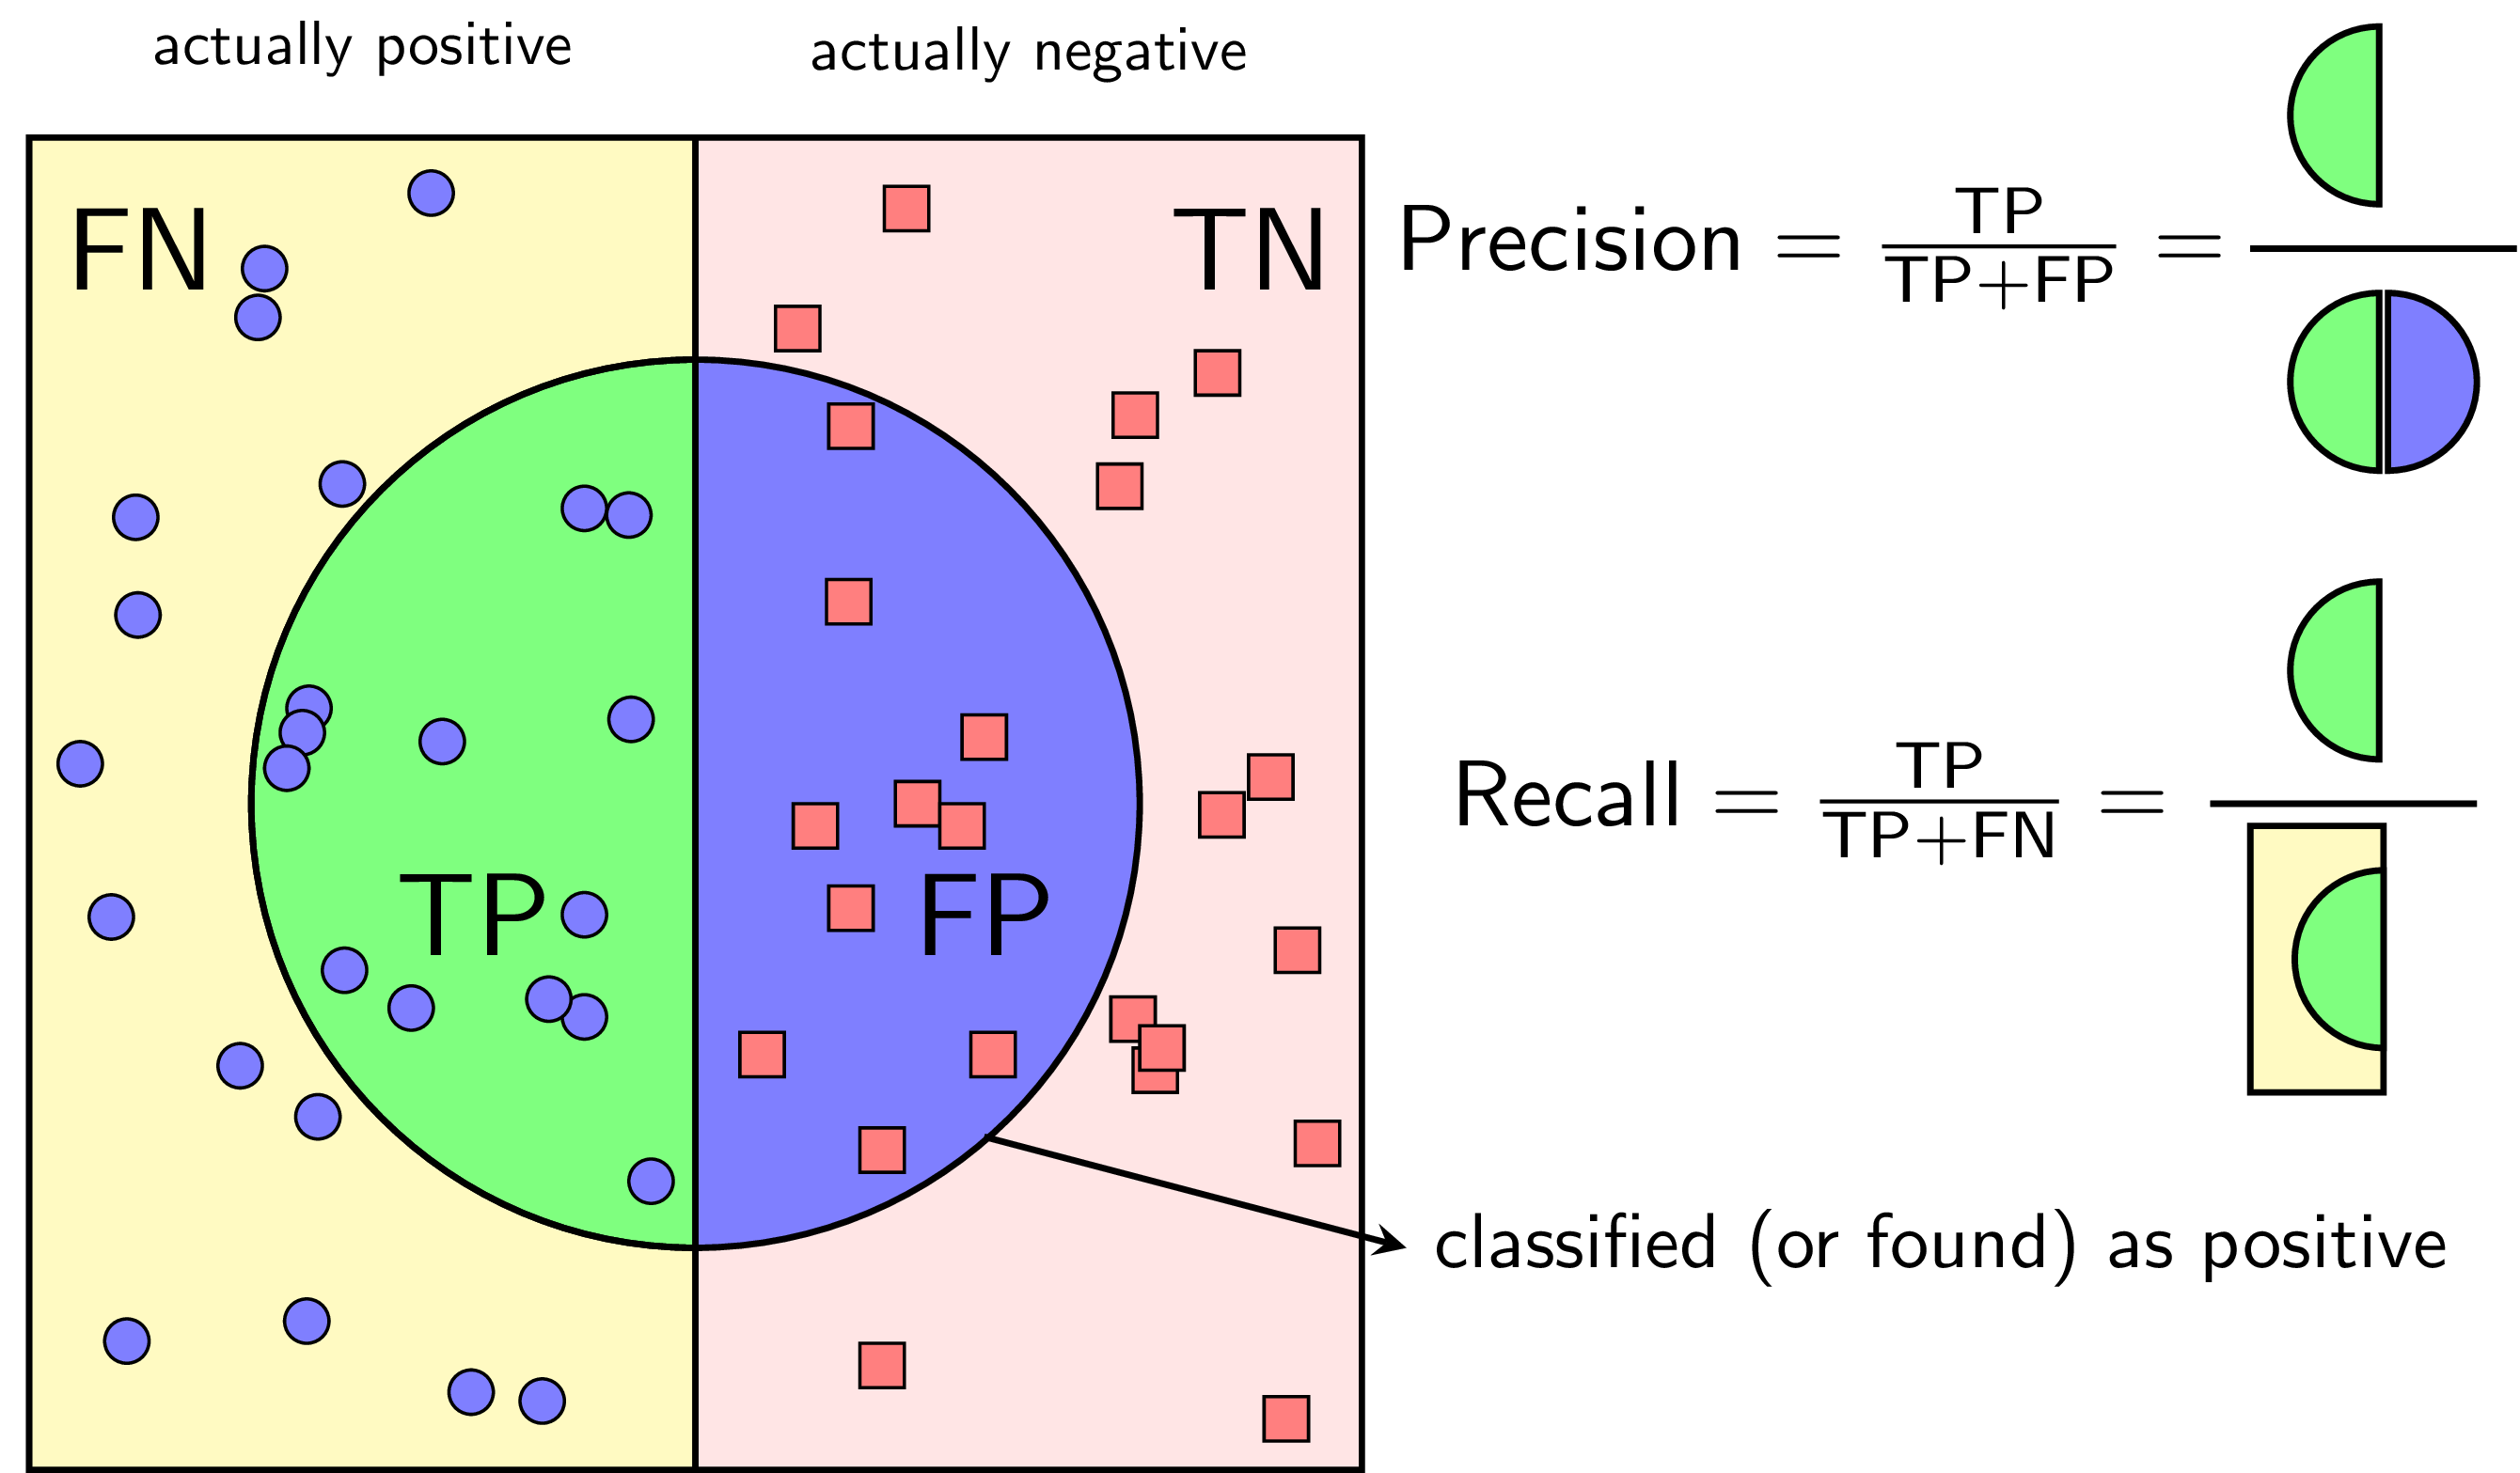
\includegraphics[scale=0.1]{hru/PR.png}
    \end{center}
    \caption{So sánh Precsion và Recall}
    \label{refhinh1}
    \end{figure}
\end{center}
\begin{mybox}
\begin{eqnarray}
\text{precision} &=& \frac{\text{TP}}{\text{TP} + \text{FP}} \\
\text{recall} &=& \frac{\text{TP}}{\text{TP} + \text{FN}}
\end{eqnarray}
\end{mybox}
Với một cách xác định một lớp là \textit{positive}, \textit{precision} được định nghĩa là tỉ lệ số điểm true positive trong số những điểm được phân loại là \textit{positive (TP + FP)}. \textit{recall} được định nghĩa là tỉ lệ số điểm \textit{true positive} trong số những điểm thực sự là \textit{positive (TP + FN)}.\\ \\
Khi \textit{precision = 1}, mọi điểm tìm được đều thực sự là \textit{positive}, tức không có điểm \textit{negative} nào lẫn vào kết quả. Tuy nhiên, \textit{precision = 1} không đảm bảo mô hình là tốt, vì câu hỏi đặt ra là liệu mô hình đã tìm được tất cả các điểm \textit{positive} hay chưa. Nếu một mô hình chỉ tìm được đúng một điểm \textit{positive} mà nó chắc chắn nhất thì ta không thể gọi nó là một mô hình tốt.\\ \\
Khi \textit{recall = 1}, mọi điểm \textit{positive} đều được tìm thấy. Tuy nhiên, đại lượng này lại không đo liệu có bao nhiêu điểm \textit{negative} bị lẫn trong đó. Nếu mô hình phân loại mọi điểm là \textit{positive} thì chắc chắn \textit{recall = 1}, tuy nhiên dễ nhận ra đây là một mô hình cực tồi.\\
\subsection{Tiêu chuẩn \textit{f1}} \\
Tiêu chuẩn \textit{f1} được định nghĩa bằng công thức như sau: \\
\begin{mybox}
$$\frac{2}{f_1} = \frac{1}{\text{precision}} + \frac{1}{\text{recall}} ~ \text{hay} ~ f_1 = 2\frac{1}{\frac{1}{\text{precision}} + \frac{1}{\text{recall}}} = 2\frac{\text{precision}\cdot{recall}}{\text{precision} + \text{recall}}$$
\end{mybox}
Nhận xét \textit{f1} càng cao, bộ phân lớp càng tốt. Khi cả \textit{recall} và precision đều bằng 1 (tốt nhất có thể) thì \textit{f1=1}.
\section{Tiêu chí lấy coreset}
Trong khuôn khổ luận văn, sau quá trình trao đổi nhóm đưa ra các tiêu chí trong việc lấy coreset như sau:
\begin{itemize}
    \item Kích thước tập coreset không vượt quá 30\% kích thước của tập gốc.
    \item Số thuộc tính của tập coreset phải bằng số thuộc tính của tập gốc.
    \item Trong tập coreset, luôn phải đầy đủ các lớp như trong tập dữ liệu gốc.
\end{itemize}
\section{Thử nghiệm trên tập dữ liệu Gender Recognition}
\subsection{Mô tả dữ liệu}
Dữ liệu này được sử dụng nhằm mục đích là nhận biết giới tính bằng phân tích giọng nói và lời nói. Cơ sở dữ liệu này được tạo ra để xác định giọng nói là nam hay nữ, dựa trên các thuộc tính âm thanh của giọng nói và lời nói. Bộ dữ liệu bao gồm 3168 mẫu giọng nói được thu âm, được thu thập từ các loa nam và nữ. Các mẫu giọng nói được xử lý trước bằng phân tích âm thanh trong ngôn ngữ R bằng cách sử dụng thư viện seewave và TuneR của R, với dải tần được phân tích là 0hz - 280hz (dải âm thanh của con người).

\subsection{Kết quả về tập dữ liệu Gender Recognition}
Đối với tập dữ liệu này, kích thước dữ liệu này tương đối nhỏ, đối với tập huấn luyện chỉ có 2534 dòng. Vì vậy, về kết quả phần coreset với tập dữ liệu này, ta tạm thời bỏ qua việc đánh giá thời gian khi chạy với tập coreset so với thời gian khi chạy hết tập dữ liệu huấn luyện. Ta sẽ đánh giá hiệu quả của việc sử dụng coreset thông qua các chỉ số: \textit{accuracy score, precision score, recall score,f1 score}.
\begin{center}
    \begin{figure}[H]
    \begin{center}
     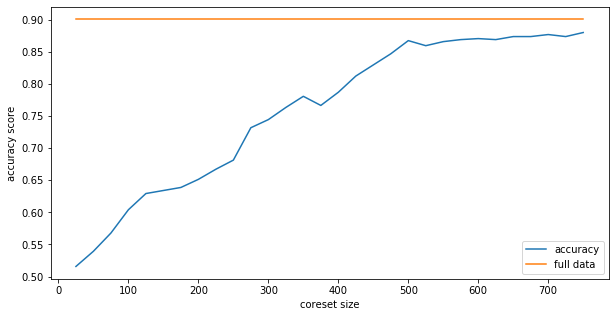
\includegraphics[scale=0.5]{accuracy_voice_gender.png}
    \end{center}
    \caption{ Minh họa accuracy score của tập coreset và tập huấn luyện gốc}
    \label{Hình 4.2}
    \end{figure}
\end{center}
Từ Hình \ref{Hình 4.2} ta thấy rằng, tập coreset có kích thước nhỏ nhất có \textit{accuracy score} dưới 55\%, trong khi đó \textit{accuracy score} của tập huấn luyện gốc thì trên 85\%. Tuy nhiên, kích thước của tập coreset càng tăng thì \textit{accuracy score} cũng tăng theo, đặc biệt là với kích thước coreset từ 500 dòng (xấp xỉ 20\% so với tập huấn luyện) trở lên, kết quả \textit{accuracy score} thu được xấp xỉ so với kết quả khi huấn luyện với tập huấn luyện gốc. Điều này cho thấy rằng, coreset thực sự có hiệu quả khi trả về \textit{accuracy score} với một kết quả xấp xỉ với kết quả tối ưu. 

\begin{center}
    \begin{figure}[H]
    \begin{center}
     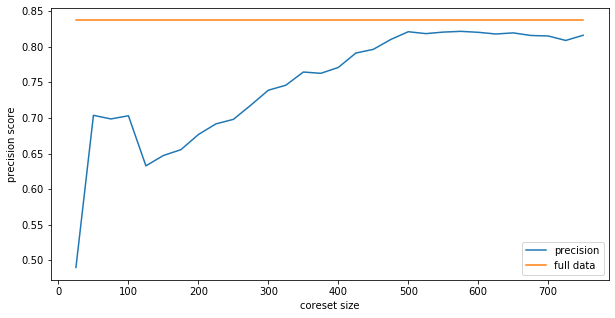
\includegraphics[scale=0.5]{precision_voice_gender.png}
    \end{center}
    \caption{Minh họa precision score của tập coreset và tập huấn luyện gốc}
    \label{Hình 4.3}
    \end{figure}
\end{center}
Từ Hình \ref{Hình 4.3} ta thấy rằng, tập coreset có \textit{precision score} thấp nhất là dưới 50\%, trong khi đó \textit{precision score} của tập huấn luyện gốc thì xấp xỉ 85\%. Tuy nhiên, kích thước của tập coreset càng tăng thì \textit{precision score} cũng tăng theo, đặc biệt là với kích thước coreset từ 500 dòng (xấp xỉ 20\% so với tập huấn luyện) trở lên, kết quả \textit{precision score} thu được xấp xỉ so với kết quả khi huấn luyện với tập huấn luyện gốc. Điều này cho thấy rằng, coreset thực sự có hiệu quả khi trả về \textit{precision score} với một kết quả xấp xỉ với kết quả tối ưu. 
\begin{center}
    \begin{figure}[H]
    \begin{center}
     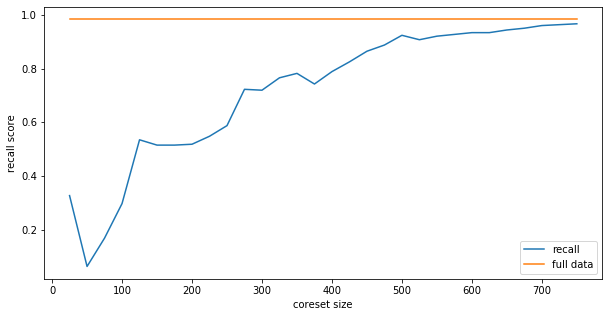
\includegraphics[scale=0.5]{recall_voice_gender.png}
    \end{center}
    \caption{Minh họa recall score của tập coreset và tập huấn luyện gốc}
    \label{Hình 4.4}
    \end{figure}
\end{center}
Từ Hình \ref{Hình 4.4} ta thấy rằng, tập coreset có \textit{recall score} nhỏ nhất là dưới 20\%, trong khi đó \textit{recall score} của tập huấn luyện gốc thì xấp xỉ 100\%. Tuy nhiên, kích thước của tập coreset càng tăng thì \textit{recall score} cũng tăng theo, đặc biệt là với kích thước coreset từ 500 dòng (xấp xỉ 20\% so với tập huấn luyện) trở lên, kết quả \textit{recall score} thu được xấp xỉ so với kết quả khi huấn luyện với tập huấn luyện gốc. Điều này cho thấy rằng, coreset thực sự có hiệu quả khi trả về \textit{recall score} với một kết quả xấp xỉ với kết quả tối ưu. 
\begin{center}
    \begin{figure}[H]
    \begin{center}
     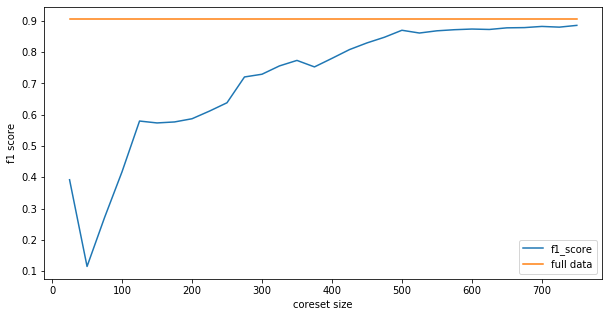
\includegraphics[scale=0.5]{f1_score_voice_gender.png}
    \end{center}
    \caption{Minh họa f1 score của tập coreset và tập huấn luyện gốc}
    \label{Hình 4.5}
    \end{figure}
\end{center}
\textit{f1 score} được tính dựa trên \textit{precision score} và \textit{recall score}, vì vậy từ Hình \ref{Hình 4.5} ta thấy rằng, tập coreset có \textit{f1 score} thấp nhất dưới 20\%, cũng là tập coreset có \textit{recall score} thấp nhất, \textit{f1 score} của tập huấn luyện gốc xấp xỉ 90\%. Tuy nhiên, kích thước của tập coreset càng tăng thì \textit{f1 score} cũng tăng theo, đặc biệt là với kích thước coreset từ 500 dòng (xấp xỉ 20\% so với tập huấn luyện) trở lên, kết quả \textit{f1 score} thu được xấp xỉ so với kết quả khi huấn luyện với tập huấn luyện gốc. Điều này cho thấy rằng, coreset thực sự có hiệu quả khi trả về \textit{f1 score} với một kết quả xấp xỉ với kết quả tối ưu.\\ \\
\textit{Precision score, recall score, f1 score} khá phổ biến trong việc đánh giá đối với các bài toán phân loại. Kết quả đánh giá dựa vào các thông số này được thể hiện thông qua các Hình \ref{Hình 4.3}, Hình \ref{Hình 4.4}, Hình \ref{Hình 4.5}, cũng tương tự như  \textit{accuracy score}, kích thước coreset càng tăng thì giá trị của các thông số cũng tăng theo. Và đặc biệt, chỉ cần 20\% đến 30\% tập huấn luyện gốc, ta đã thu được kết quả xấp xỉ với kết quả tối ưu. 
\section{Thử nghiệm trên tập dữ liệu Skin Segmentation}
\subsection{Mô tả dữ liệu}
Bộ dữ liệu Skin Segmentation được thu thập bằng cách lấy mẫu ngẫu nhiên các giá trị R(Red), G(Green), B(Blue) từ hình ảnh khuôn mặt của các nhóm tuổi khác nhau (trẻ, trung bình và già), các nhóm chủng tộc (trắng, đen và châu Á) và giới tính thu được từ cơ sở dữ liệu FERET và cơ sở dữ liệu PAL. Tổng kích thước mẫu học tập là 245057; trong đó 50859 là mẫu da và 194198 là mẫu không phải da. Cơ sở dữ liệu hình ảnh màu FERET (\cite {Color Database}), Cơ sở dữ liệu PAL Face từ Phòng thí nghiệm lão hóa năng suất, Đại học Texas tại Dallas (\cite{Face Database}). Tập dữ liệu này có kích thước 245057 * 4 trong đó ba cột đầu tiên là các giá trị B, G, R (x1, x2 và x3) và cột thứ tư là nhãn của dữ liệu.
\subsection{Kết quả về thời gian huấn luyện của tập coreset và tập huấn luyện gốc}
\begin{center}
    \begin{figure}[H]
    \begin{center}
     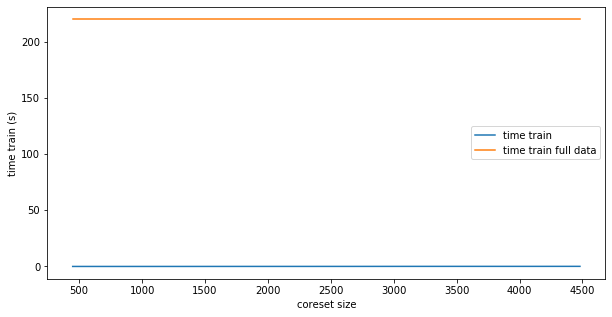
\includegraphics[scale=0.55]{time_train_skin.png}
    \end{center}
    \caption{Thời gian huấn luyện của tập coreset và tập huấn luyện gốc}
    \label{Hình 4.6}
    \end{figure}
\end{center}
Từ Hình \ref{Hình 4.6} thấy rằng, thời gian huấn luyện của tập coreset nhỏ hơn rất nhiều so với tập huấn luyện gốc.
\subsection{Kết quả về sự hiệu quả của coreset trên Skin Segmentation }
\begin{center}
    \begin{figure}[H]
    \begin{center}
     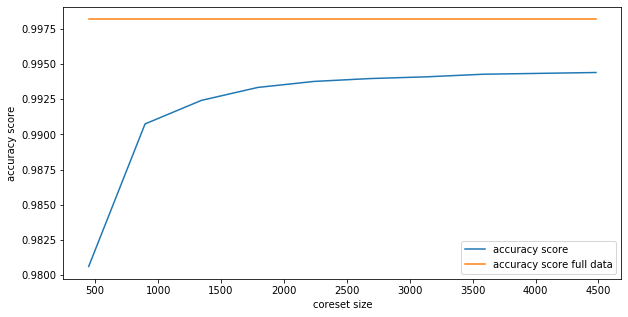
\includegraphics[scale=0.5]{accuracy_skin.png}
    \end{center}
    \caption{Minh họa accuracy score của tập coreset và tập huấn luyện gốc}
    \label{Hình 4.7}
    \end{figure}
\end{center}
Từ Hình \ref{Hình 4.7} ta thấy rằng, tập coreset có kích thước nhỏ nhất có \textit{accuracy score} trên 98\%, trong khi đó \textit{accuracy score} của tập huấn luyện gốc thì trên 99.75\%. Điều này cho ta thấy được \textit{accuracy score} giữa tập coreset và tập huấn luyện gốc không quá chênh lệch. Thêm vào đó, kích thước của tập coreset càng tăng thì \textit{accuracy score} cũng tăng theo, đặc biệt là chỉ với 3\% 
dữ liệu huấn luyện gốc đã thu được kết quả \textit{accuracy score} xấp xỉ so với kết quả khi huấn luyện với tập huấn luyện gốc. Điều này cho thấy rằng, coreset thực sự có hiệu quả khi trả về \textit{accuracy score} với một kết quả xấp xỉ với kết quả tối ưu. 
\begin{center}
    \begin{figure}[H]
    \begin{center}
     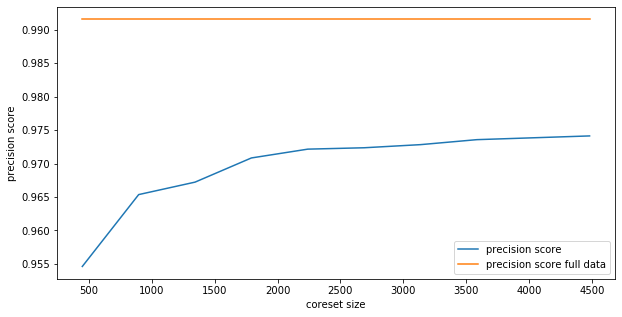
\includegraphics[scale=0.5]{precision_skin.png}
    \end{center}
    \caption{Minh họa precision score của tập coreset và tập huấn luyện gốc}
    \label{Hình 4.8}
    \end{figure}
\end{center}
Từ Hình \ref{Hình 4.8} ta thấy rằng, tập coreset có kích thước nhỏ nhất có \textit{precision score} trên 95\%, trong khi đó \textit{precision score} của tập huấn luyện gốc thì trên 99\%. Thêm vào đó, kích thước của tập coreset càng tăng thì \textit{precision score} cũng tăng theo, đặc biệt là chỉ với 3\% dữ liệu huấn luyện gốc đã thu được kết quả \textit{precision score} xấp xỉ so với kết quả khi huấn luyện với tập huấn luyện gốc. Điều này cho thấy rằng, coreset thực sự có hiệu quả khi trả về \textit{precision score} với một kết quả xấp xỉ với kết quả tối ưu. 
\begin{center}
    \begin{figure}[H]
    \begin{center}
     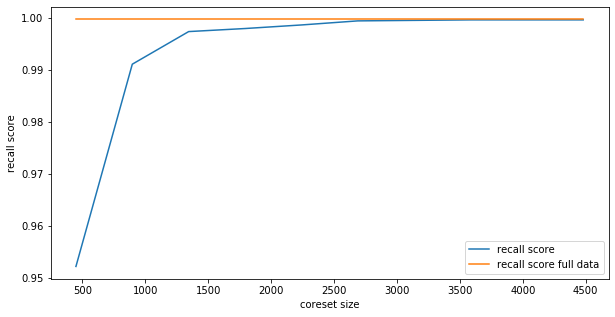
\includegraphics[scale=0.4]{recall_skin.png}
    \end{center}
    \caption{Minh họa recall score của tập coreset và tập huấn luyện gốc}
    \label{Hình 4.9}
    \end{figure}
\end{center}
Theo Hình \ref{Hình 4.9} ta thấy rằng, tập coreset có kích thước nhỏ nhất có \textit{recall score} trên 95\%, trong khi đó \textit{precision score} của tập huấn luyện gốc thì 100\%. Thêm vào đó, kích thước của tập coreset càng tăng thì \textit{recall score} cũng tăng theo, đặc biệt là chỉ với 3\% dữ liệu huấn luyện gốc đã thu được \textit{recall score} xấp xỉ so với kết quả khi huấn luyện với tập huấn luyện gốc. Điều này cho thấy rằng, coreset thực sự có hiệu quả khi trả về \textit{recall score} với một kết quả xấp xỉ với kết quả tối ưu. 
\begin{center}
    \begin{figure}[H]
    \begin{center}
     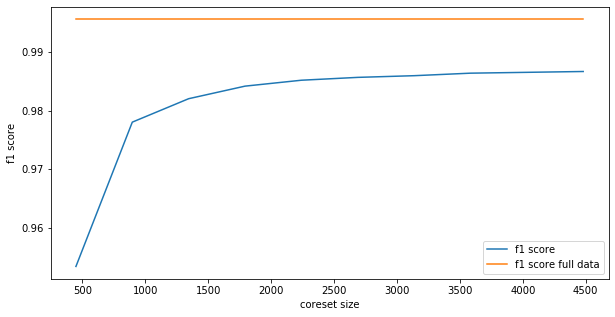
\includegraphics[scale=0.4]{f1_score_skin.png}
    \end{center}
    \caption{Minh họa f1 score của tập coreset và tập huấn luyện gốc}
    \label{Hình 4.10}
    \end{figure}
\end{center}
\textit{f1 score} được tính dựa trên \textit{precision score} và \textit{recall score}, vì vậy từ Hình \ref{Hình 4.10} ta thấy rằng, tập coreset có \textit{f1 score} thấp nhất dưới 96\%, còn \textit{f1 score} của tập huấn luyện gốc trên 99\%. Tuy nhiên, kích thước của tập coreset càng tăng thì \textit{f1 score} cũng tăng theo, đặc biệt là chỉ với 3\% dữ liệu huấn luyện gốc đã thu được \textit{f1 score} xấp xỉ so với kết quả khi huấn luyện với tập huấn luyện gốc. Điều này cho thấy rằng, coreset thực sự có hiệu quả khi trả về \textit{f1 score} với một kết quả xấp xỉ với kết quả tối ưu.\\ \\
\textit{Accuracy score, precision score, recall score, f1 score} khá phổ biến trong việc đánh giá đối với các bài toán phân loại. Kết quả của các thông số này được mô tả lần lượt trong các Hình \ref{Hình 4.7}, Hình \ref{Hình 4.8}, Hình \ref{Hình 4.9} và Hình \ref{Hình 4.10}, ta thấy rằng kích thước coreset càng tăng thì giá trị của các thông số cũng tăng theo. Và đặc biệt, chỉ cần khoảng 3\% tập huấn luyện gốc, ta đã thu được kết quả xấp xỉ với kết quả tối ưu (chênh lệch trong khoảng 2\%) mà thời gian huấn luyện của tập coreset lại nhỏ hơn gấp nhiều lần so với khi huấn luyện với tập huấn luyện gốc.

\section{Thử nghiệm trên tập dữ liệu HTRU2}
\subsection{Mô tả dữ liệu}
HTRU2 là một bộ dữ liệu mô tả một mẫu các ứng cử viên xung (Pulsar) được thu thập trong High Time Resolution Universe Survey. Pulsar là một loại sao neutron hiếm hoi tạo ra phát xạ vô tuyến có thể phát hiện được ở đây trên Trái đất. Chúng được quan tâm bởi giới  khoa học đáng kể như các đầu dò của không-thời gian, môi trường liên sao và trạng thái của vật chất (xem [2] để sử dụng nhiều hơn).\\
Khi các pulsar quay, chùm phát xạ của chúng quét khắp bầu trời và khi điều này vượt qua tầm nhìn của chúng ta, sẽ tạo ra một mô hình phát xạ vô tuyến băng rộng có thể phát hiện được. Như pulsar xoay nhanh, mô hình này lặp lại định kỳ. Do đó, tìm kiếm xung bao gồm tìm kiếm các tín hiệu vô tuyến định kỳ với các kính thiên văn vô tuyến lớn.\\ \\
Mỗi pulsar tạo ra một kiểu phát xạ hơi khác nhau, thay đổi một chút theo từng vòng quay (xem [2] để biết giới thiệu về vật lý thiên văn pulsar để tìm hiểu lý do tại sao). Do đó, một phát hiện tín hiệu tiềm năng được gọi là 'ứng cử viên', được tính trung bình trên nhiều vòng quay của pulsar, như được xác định bởi độ dài của một quan sát. Trong trường hợp không có thêm thông tin, mỗi ứng viên có khả năng mô tả một pulsar thực sự. Tuy nhiên, trong thực tế, hầu hết các phát hiện đều do nhiễu tần số vô tuyến (RFI) và nhiễu, làm cho các tín hiệu hợp pháp khó tìm thấy.\\ \\
Các công cụ học máy hiện đang được sử dụng để tự động dán nhãn cho các ứng cử viên pulsar để tạo điều kiện cho việc phân tích nhanh chóng. Hệ thống phân loại nói riêng đang được áp dụng rộng rãi, coi các tập dữ liệu ứng cử viên là các vấn đề phân loại nhị phân. Ở đây các ví dụ pulsar hợp pháp là một lớp tích cực thiểu số, và các ví dụ giả là lớp phủ định đa số. Hiện tại các nhãn đa lớp không có sẵn, do các chi phí liên quan đến chú thích dữ liệu.\\ \\
Tập dữ liệu được chia sẻ ở đây chứa 16.259 ví dụ giả gây ra bởi RFI/nhiễu và 1.639 ví dụ xung thực. Những ví dụ này đã được kiểm tra bởi các chú thích của con người. Với tập dữ liệu này, nhóm đã thử nghiệm huấn luyện với các \textit{kernel} khác nhau nhằm đánh giá kết quả của tập dữ liệu khi huấn luyện với các \textit{kernel} khác nhau như thế nào.
\subsection{Kết quả về thời gian train trên tập HTRU2}
\begin{center}
    \begin{figure}[H]
    \begin{center}
     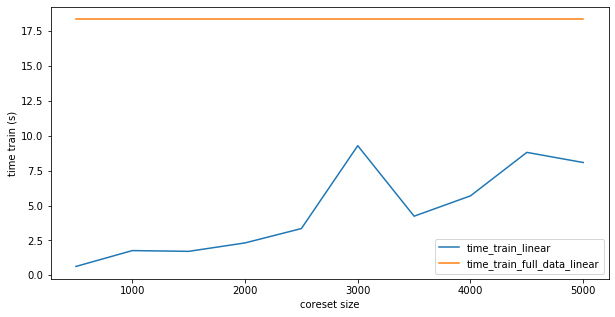
\includegraphics[scale=0.4]{HTRU2_1.png}
    \end{center}
    \caption{Thời gian train khi train với kernel linear}
    \label{Hình 4.11}
    \end{figure}
\end{center}
\begin{center}
    \begin{figure}[H]
    \begin{center}
     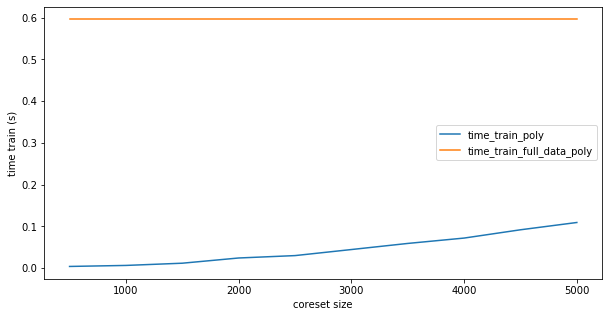
\includegraphics[scale=0.4]{HTRU2_2.png}
    \end{center}
    \caption{Thời gian train khi train với kernel polynomial}
    \label{Hình 4.12}
    \end{figure}
\end{center}
\begin{center}
    \begin{figure}[H]
    \begin{center}
     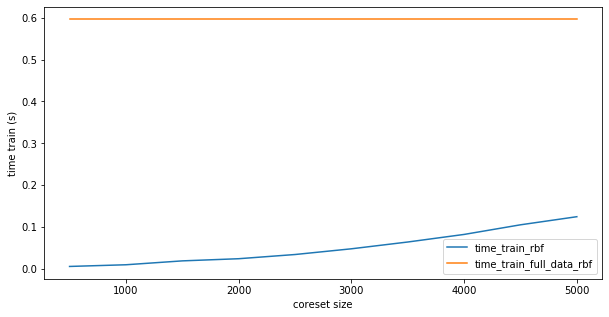
\includegraphics[scale=0.4]{HTRU2_3.png}
    \end{center}
    \caption{Thời gian train khi train với kernel rbf}
    \label{Hình 4.13}
    \end{figure}
\end{center}

Từ các Hình \ref{Hình 4.11}, Hình \ref{Hình 4.12}, Hình \ref{Hình 4.13} , ta đều thấy rằng thời gian huấn luyện với các tập coreset đều nhỏ hơn rất nhiều so với khi huấn luyện với tập huấn luyện gốc. Thời gian huấn luyện giữa các kernel có sự khác biệt, điều này liên quan đến phần hiện thực cũng như giải thuật của các kernel. Nhìn chung, nếu ta huấn luyện các tập coreset, ta có thể tiết kiệm rất nhiều thời gian thay vì đi huấn luyện với tập huấn luyện gốc. 

\subsection{Kết quả về sự hiệu quả của coreset trên tập HTRU2}
\begin{center}
    \begin{figure}[H]
    \begin{center}
     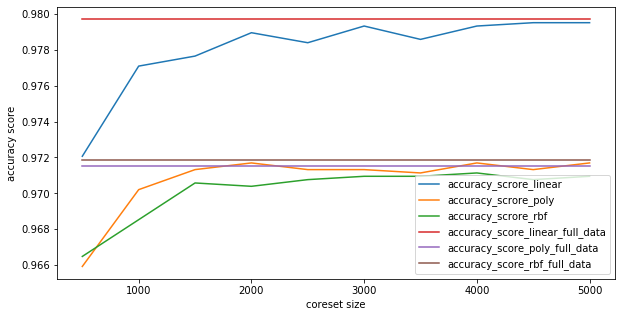
\includegraphics[scale=0.4]{HTRU2_4.png}
    \end{center}
    \caption{Minh họa accuracy khi so sánh các kernel}
    \label{Hình 4.14}
    \end{figure}
\end{center}
Nhìn vào Hình \ref{Hình 4.14}, ta thấy kết quả khi huấn luyện với kernel linear tốt hơn so với hai kernel khác, tuy nhiên kết quả giữa các kernel với nhau không quá chênh lệch. Về kết quả giữa các coreset, ta cũng thấy được rằng kết quả khi huấn luyện tập coreset với các kernel cũng giống như giống với khi huấn luyện với tập huấn luyện gốc, đều cho thấy kernel linear tốt hơn so với hai kernel còn lại. Còn về kết quả khi huấn luyện với tập coreset, thì kết quả thu được càng xấp xỉ so với kết quả tối ưu khi tăng kích thước coreset lên. Nhưng nhìn chung, kết quả khi huấn luyện với tập coreset không quá chênh lệch với khi huấn luyện với tập huấn luyện gốc. 
\begin{center}
    \begin{figure}[H]
    \begin{center}
     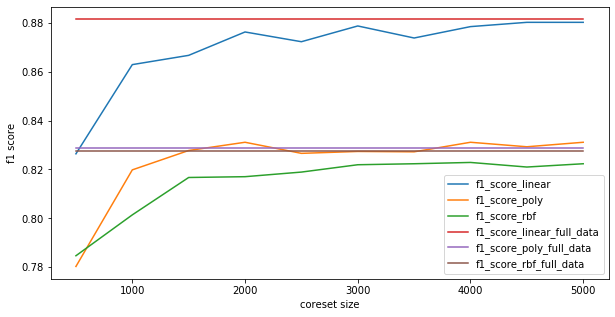
\includegraphics[scale=0.4]{HTRU2_5.png}
    \end{center}
    \caption{Minh họa f1 khi so sánh các kernel}
    \label{Hình 4.15}
    \end{figure}
\end{center}
\begin{center}
    \begin{figure}[H]
    \begin{center}
     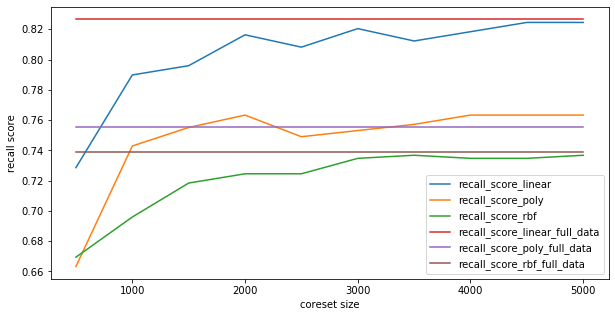
\includegraphics[scale=0.4]{HTRU2_6.png}
    \end{center}
    \caption{Minh họa recall khi so sánh các kernel}
    \label{Hình 4.16}
    \end{figure}
\end{center}
\begin{center}
    \begin{figure}[H]
    \begin{center}
     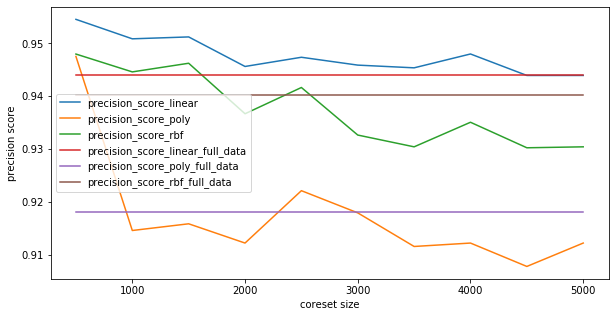
\includegraphics[scale=0.4]{HTRU2_7.png}
    \end{center}
    \caption{Minh họa precision khi so sánh các kernel}
    \label{Hình 4.17}
    \end{figure}
\end{center}

Kết quả về các đánh giá như \textit{precision score, recall score, f1 score} được mô tả ở các Hình \ref{Hình 4.15}, Hình \ref{Hình 4.16} và Hình \ref{Hình 4.17}. Cũng tương tự như phần đánh giá về \textit{accuracy score}, kết quả từ các hình trên cũng cho thấy kết quả khi huấn luyện với kernel linear cao hơn so với hai kernel còn lại. Thêm vào đó, kết quả khi chạy với tập coreset cũng xấp xỉ với khi chạy với tập dữ liệu lớn. 

\section{Nhận xét}
Từ những tập dữ liệu được thực nghiệm ở Chương 4, đã cho ta thấy được hiệu quả của coreset khi áp dụng vào mô hình SVM trong bài toán phân lớp. Cụ thể như sau, thứ nhất là về mặt thời gian, thời gian khi huấn luyện với các tập coreset nhỏ hơn rất nhiều so với khi huấn luyện với dữ liệu gốc. Thứ hai, khi sử dụng các tập coreset, kích thước các tập coreset nhỏ hơn rất nhiều nhưng ta thu được kết quả xấp xỉ với kết quả khi huấn luyện với dữ liệu gốc. Thêm vào đó, khi huấn luyện các tập coreset với các kernel khác nhau, thì cũng cho thấy được kết quả khi huấn luyện giữa các kernel cũng giống như khi huấn luyện với dữ liệu gốc, cụ thể là kernel nào tốt hơn cho bài toán, kernel nào không phù hợp,... điều đó đã thể hiện khi huấn luyện bằng các tập coreset, không cần phải huấn luyện với tập dữ liệu gốc mới có thể biết được điều đó.  
\chapter{Áp dụng vào các bài toán thực tế}
\section{Ứng dụng cho bài toán phòng chống gian lận}
\subsection{Mô tả bài toán}
Hiện nay, đi kèm với sự phát triển về kinh tế, công nghệ,... nhu cầu sử dụng tiền mặt của con người trở nên ít đi, thay vào đó là sự xuất hiện thói quen sử dụng tiền tệ theo nhiều cách khác nhau. Một trong số đó là việc sử dụng thẻ tín dụng trong các giao dịch thanh toán. Tuy nhiên, bên cạnh những lợi ích khi sử dụng thẻ tín dụng, thì có những rủi ro kèm theo, đặc biệt là: thông tin thẻ bị lộ dẫn đến thẻ tín dụng được sử dụng bởi người khác mà không có sự cho phép của chủ thẻ, những giao dịch như thế này gọi là những giao dịch gian lận. Chính vì vậy, việc có thể phát hiện và ngăn chặn những giao dịch gian lận luôn là mục tiêu hàng đầu trong việc bảo vệ người dùng của các ngân hàng. Vì vậy bài toán đặt ra chính là làm sao có thể phát hiện ra các giao dịch gian lận và ngăn chặn chúng. \\ \\ 
Đối với ngân hàng, trong việc phòng chống các giao dịch gian lận, cứ mỗi giao dịch thanh toán sẽ được phân thành hai loại giao dịch: giao dịch không gian lận và giao dịch gian lận. Đây là tiền đề cho bài toán phân lớp. Như ta đã biết, số lượng giao dịch thanh toán của ngân hàng rất là lớn, vì vậy việc sử dụng hết các giao dịch này để huấn luyện tốn rất nhiều thời gian. Chính vì thế, việc sử dụng coreset để lấy một tập mẫu cho việc huấn luyện là một giải pháp hiệu quả cho bài toán này.\\ \\
Hiện nay, giải thuật coreset mà nhóm đang sử dụng chưa có sự tối ưu về mặt thời gian. Vì vậy, trong khuôn khổ luận văn, nhóm lấy một tập dữ liệu với kích thước vừa đủ để thể hiện sự hiệu quả của coreset và mô hình SVM cho ứng dụng này. 

\subsection{Mô tả tập dữ liệu}
Tập dữ liệu này chứa các giao dịch được thực hiện bằng thẻ tín dụng vào tháng 9 năm 2013 của các chủ thẻ ở Châu Âu. Tập này chứa các giao dịch trong hai ngày, bao gồm 492 giao dịch gian lận trong tổng số 284807 giao dịch.\\ \\
Vì vấn đề về bảo mật nên không thể cung cấp các đặc trưng (feature) gốc cũng như thông tin của người dùng , nên tập dữ liệu này là kết quả của việc sử dụng phương pháp PCA. Các đặc trưng từ V1 đến V28 là các đặc trưng thu được từ phương pháp PCA. Đặc trưng class chính là nhãn của tập dữ liệu với giá trị 1 là giao dịch gian lận và 0 là giao dịch không gian lận.\\ \\
Như đã đề cập ở phần mô tả bài toán, vì lý do hiện tại giải thuật coreset vẫn chưa tối ưu về mặt thời gian, nên từ tập dữ liệu trên, nhóm sẽ lấy một phần nhỏ khoảng 20000 dòng để mô tả ứng dụng của coreset và mô hình SVM vào bài toán này.

\subsection{Phân tích tập dữ liệu}
\begin{center}
    \begin{figure}[H]
    \begin{center}
     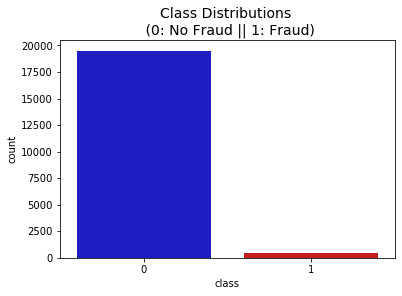
\includegraphics[scale=0.6]{creditCardFraud_distribution_class.png}
    \end{center}
    \caption{Phân bố (distribution) của các giao dịch trong tập dữ liệu}
    \label{Hình 5.1}
    \end{figure}
\end{center}
Từ hình vẽ \ref{Hình 5.1}, ta thấy rằng dữ liệu hiện tại mất cân bằng. Chỉ có khoảng 492 giao dịch gian lận trong tổng số 20000 giao dịch. Tuy nhiên, trên thực tế, tỷ lệ mất cân bằng như thế này là một điều hợp lý. Đối với dữ liệu mất cân bằng, ta sử dụng một số độ đo như \textit{precison,recall, f1 score} để đánh giá thay vì chỉ sử dụng \textit{accuracy score}.\\

\begin{center}
    \begin{figure}[H]
    \begin{center}
     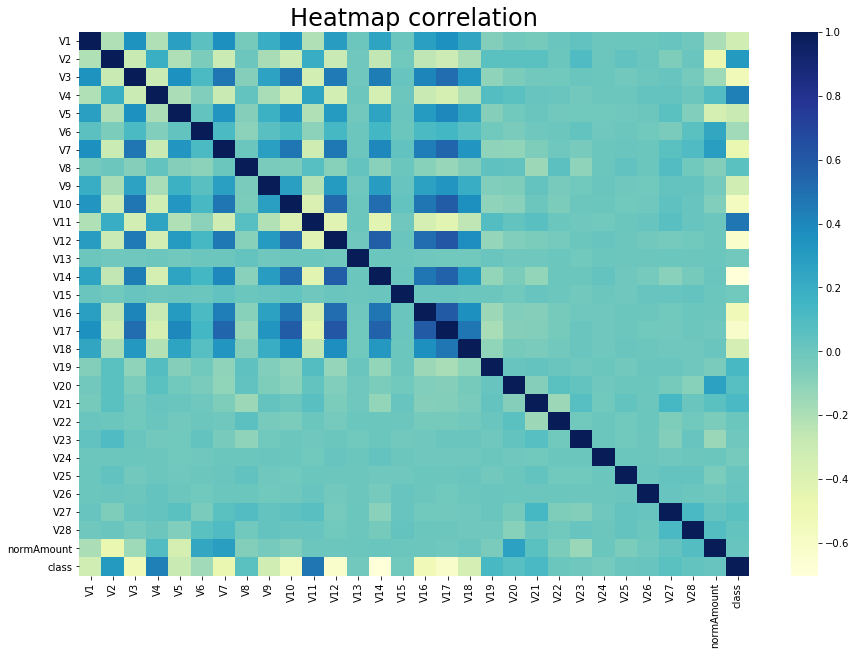
\includegraphics[scale=0.3]{correlation_creditcard_fraud.png}
    \end{center}
    \caption{Biểu đồ tương quan của các thuộc tính dữ liệu với nhãn}
    \label{Hình 5.2}
    \end{figure}
\end{center}
Từ hình \ref{Hình 5.2}, ta thấy hầu hết các đặc trưng không có sự tương quan với nhau. Điều này cho thấy rằng phương pháp PCA đã được thực hiện trước đó. Thực tế phương pháp PCA đã được sử dụng, vì vậy trong trường hợp này chúng ta sẽ không thực hiện việc giảm kích thước tại tập dữ liệu này nữa. Ngoài ra, ta thấy rằng một số đặc trưng V17,V14,V12 và V10 có mối quan hệ tương quan nghịch. Giá trị càng thấp thì kết quả cuối cùng sẽ là một giao dịch gian lận. Các đặc trưng V2,V4,V11 và V19 có quan hệ tương quan thuận. Giá trị càng cao thì kết quả cuối cùng sẽ là một giao dịch gian lận. Ta sử dụng biểu đồ hộp (boxplot) để có thể hiệu rõ hơn về sự phân bố của các đặc trưng trong giao dịch gian lận và giao dịch không gian lận. Kết quả được trình bày ở Hình 5.3  và Hình 5.4.

\begin{center}
    \begin{figure}[H]
    \begin{center}
     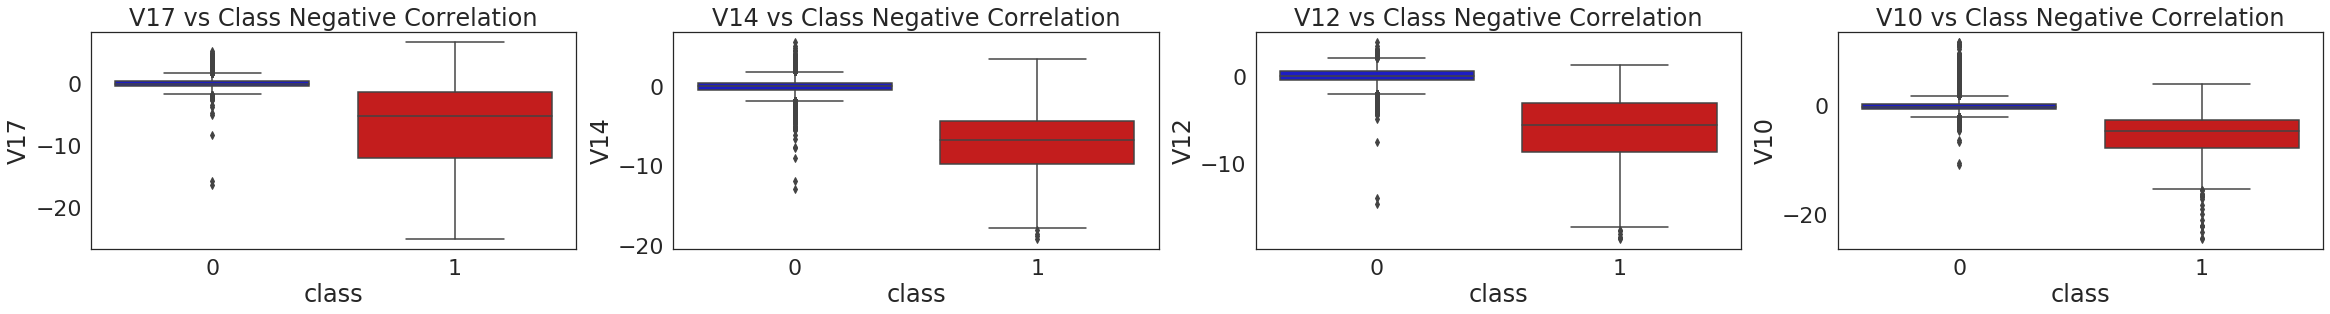
\includegraphics[scale=0.2]{feature_class_negative_correlation.png}
     \caption{Biểu đồ tương quan thuộc tính và lớp Negative}
    \end{center}
    \label{Hình 5.3}
    \end{figure}
\end{center}
\begin{center}
    \begin{figure}[H]
    \begin{center}
     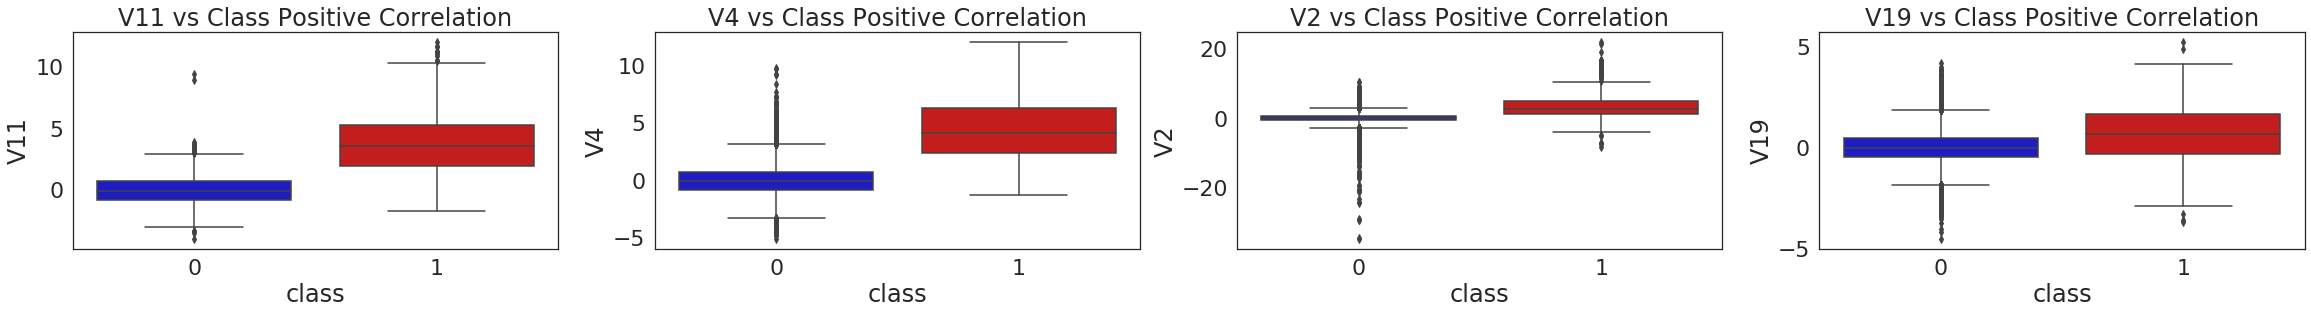
\includegraphics[scale=0.2]{feature_class_positive_correlation.png}
     \caption{Biểu đồ tương quan thuộc tính và lớp Positive}
    \end{center}
    \label{Hình 5.4}
    \end{figure}
\end{center}
Ta chia tập dữ liệu này thành hai tập là tập huấn luyện và tập kiểm thử theo tỷ lệ 4:1. Đồng thời, ta thực hiện việc lấy coreset từ tập huấn luyện và dùng tập kiểm thử để đánh giá sự hiệu quả của coreset.

\subsection{Ứng dụng coreset vào bài toán}
Với phần ứng dụng, ta chỉ đưa ra kết quả khi chạy với các tập coreset để cho thấy được mức độ hiệu quả của nó. Từ tập huấn luyện, ta thực hiện việc lấy các tập coreset ứng với kích thước từ 0.5\% đến 30\% so với tập huấn luyện. Kết quả được đánh giá dựa vào các chỉ số như: \textit{precision, recall, f1 score, accuracy score} và thời gian huấn luyện các tập coreset ứng với các kernel linear, polynomial và rbf.\\

\begin{center}
    \begin{figure}[H]
    \begin{center}
     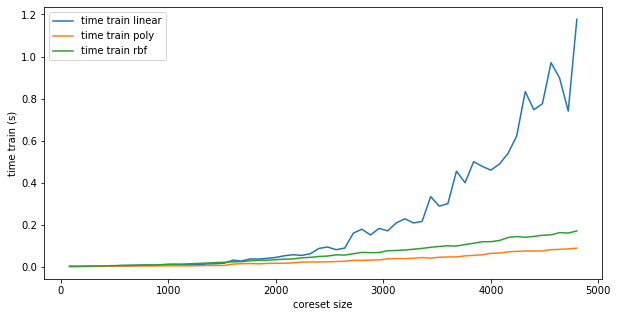
\includegraphics[scale=0.4]{timetrain_creditcard_fraud.png}
    \end{center}
     \caption{Thời gian huấn luyện ứng của tập coreset ứng với các kernel}
    \label{Hình 5.5}
    \end{figure}
\end{center}
Nhìn vào hình \ref{Hình 5.5}, ta thấy rằng thời gian huấn luyện có xu hướng tăng theo kích thước tập coreset, thời gian huấn luyện với kernel linear thì lớn hơn so với hai kernel còn lại. Điều này phụ thuộc vào cách hiện thực của các kernel. Tuy nhiên, thời gian huấn luyện tương đối nhỏ. 
\begin{center}
    \begin{figure}[H]
    \begin{center}
     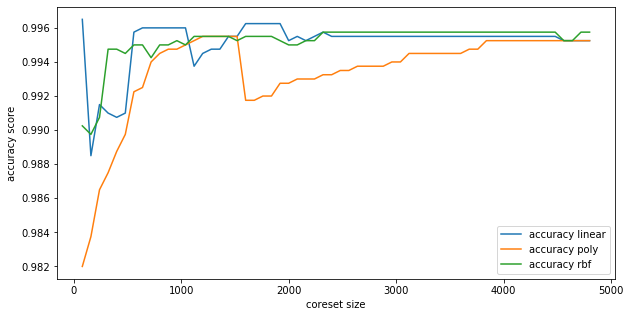
\includegraphics[scale=0.4]{accuracy_creditcard_Fraud.png}
    \end{center}
     \caption{Minh họa accuracy score của tập coreset ứng với các kernel}
    \label{Hình 5.6}
    \end{figure}
\end{center}
Kết quả \textit{accuracy score} được thể hiện ở Hình \ref{Hình 5.6}, nhìn chung ta thấy kết quả khi chạy với tập coreset với kết quả khi chạy với tập huấn luyện gốc không quá chênh lệch. Với kích thước coreset dưới 2000 dòng, ta thấy kết quả có sự biến thiên. Tuy nhiên, kết quả trở nên tốt hơn với kích thước coreset trên 2000 dòng. 
\begin{center}
    \begin{figure}[H]
    \begin{center}
     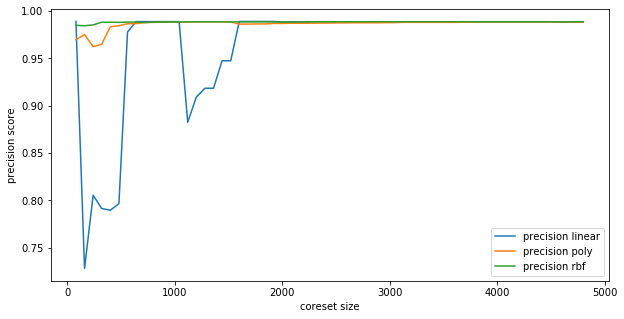
\includegraphics[scale=0.4]{precision_creditcard_Fraud.png}
    \end{center}
     \caption{Minh họa precision score của tập coreset ứng với các kernel}
    \label{Hình 5.7}
    \end{figure}
\end{center}
\begin{center}
    \begin{figure}[H]
    \begin{center}
     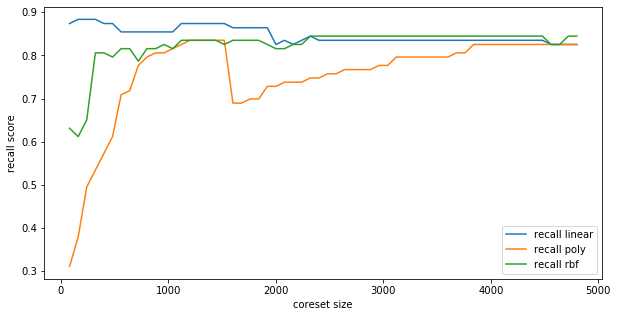
\includegraphics[scale=0.4]{recall_creditcard_Fraud.png}
    \end{center}
     \caption{ Minh họa recall score của tập coreset ứng với các kernel}
    \label{Hình 5.8}
    \end{figure}
\end{center}
\begin{center}
    \begin{figure}[H]
    \begin{center}
     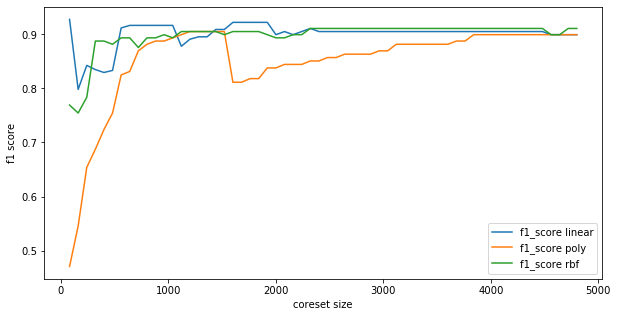
\includegraphics[scale=0.4]{f1_score_creditcard_Fraud.png}
    \end{center}
     \caption{Minh họa f1 score của tập coreset ứng với các kernel}
    \label{Hình 5.9}
    \end{figure}
\end{center}
\textit{precision score, recall score, f1 score} khá phổ biến trong việc đánh giá đối với các bài toán phân loại. Ở trong bài toán này, kết quả của các thông số được thể hiện ở Hình \ref{Hình 5.7}, Hình \ref{Hình 5.8} và Hình \ref{Hình 5.9}. Từ đây ta thấy rằng, cũng tương tự như accuracy score, kích thước coreset càng tăng thì giá trị của các thông số cũng tăng theo. Và đặc biệt, chỉ cần 20\% đến 30\% tập huấn luyện gốc, ta đã thu được kết quả xấp xỉ với kết quả tối ưu.\\ \\
Từ những kết quả trên, ta thấy rằng: thời gian huấn luyện của các tập coreset ứng với các kernel có sự khác nhau, thời gian huấn luyện của kernel linear cao hơn so với hai kernel khác. Đối với các coreset có kích thước dưới 2000 dòng, thì nhìn chung các chỉ số đánh giá về \textit{precision, recall, accuracy score} chưa ổn định, tuy nhiên \textit{precision} vẫn rất cao (trên 98\%). Kích thước coreset càng lớn thì khả năng phân loại càng tốt, và các chỉ số đánh giá có sự hội tụ khi kích thước coreset tăng. Với những chứng minh về sự hiệu quả của coreset đã được đưa ra ở chương trước, kết quả này càng thể hiện rõ được sự hiệu quả của nó, khi chỉ cần sử dụng khoảng 10\% đến 20\% dữ liệu đã thu được một kết quả khá tốt. Điều này cho thấy, nếu huấn luyện với tập dữ liệu gốc, kết quả thu được cùng rất khả quan.\\
Để có thể cho thấy kết quả của coreset và SVM trong ứng dụng này, nhóm sử dụng tập coreset có kích thước bằng 20\% so với tập dữ liệu huấn luyện. Kết quả của \textit{confusion matrix} được thể hiện ở Hình \ref{Hình 5.10} :
\begin{center}
    \begin{figure}[H]
    \begin{center}
     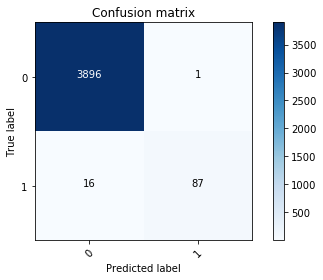
\includegraphics[scale=0.5]{Confusion_matrix_creditCardFraud.png}
    \end{center}
    \caption {Confusion Matrix tập Credit Card Fraud}
    \label{Hình 5.10}
    \end{figure}
\end{center}
Từ kết quả hình \ref{Hình 5.10}, ta tính ra được \textit{precision} = 98.86\% và \textit{recall} = 84.47\%. Nếu sử dụng mô hình SVM và coreset, thì phía ngân hàng đã ngăn chặn được 87 giao dịch gian lận trong tổng số 103 giao dịch gian lận. Số giao dịch ngăn chặn sai là 1. Kết quả này sẽ giúp cho việc cải thiện khả năng bảo vệ người dùng của họ trước những tác nhân gây nguy hiểm khi sử dụng thẻ tín dụng. Đồng thời, cũng giúp cho ngân hàng giảm tải được những cuộc gọi khiếu nại cũng như báo cáo lộ thông tin thẻ bên phía bộ phận chăm sóc khách hàng ở ngân hàng.

\section{Ứng dụng cho bài toán phân biệt giới tính dựa trên ảnh khuôn mặt}
\subsection{Mô tả bài toán}
Theo Thông tư 23/2019/TT-NHNN, đối với ví điện tử của cá nhân, cá nhân là người Việt Nam phải cung cấp những thông tin gồm: Họ và tên; ngày, tháng, năm sinh; quốc tịch; số điện thoại; số căn cước công dân hoặc số chứng minh nhân dân hoặc số hộ chiếu còn thời hạn, ngày cấp, nơi cấp. Còn đối với cá nhân là người nước ngoài, thông tin gồm: Họ và tên; ngày, tháng, năm sinh; quốc tịch; số điện thoại; số hộ chiếu còn thời hạn, ngày cấp, nơi cấp, thị thực nhập cảnh (nếu có). Việc áp dụng thông tư này đối với các ví điện tử trở thành một bài toán lớn và ưu tiên hàng đầu. Theo cách truyền thống, việc xác thực người dùng thường được một nhóm người thực hiện bằng hình thức thủ công. Tuy nhiên, với số lượng người dùng lên tới hàng triệu người, việc đồng loạt xử lý những yêu cầu trở thành một vấn đề lớn cho các ví điện tử hiện nay. Vậy nên, việc áp dụng các công nghệ trong việc xác thực người dùng được quan tâm đến. Có rất nhiều bước xác thực người dùng, ví dụ như: xác thực giới tính của người dùng trong CMND và ảnh người dùng chụp, xác thực ảnh trong CMND và ảnh hiện tại có giống nhau hay không, xác thực các thông tin liên quan khác,... Việc xác thực giới tính của người dùng thông qua ảnh khuôn mặt là một trong những bài toán cần giải quyết ở đây.\\
Chính vì vậy, nhóm quyết định sử dụng coreset và mô hình SVM trong việc phân biệt giới tính của người dùng thông qua ảnh khuôn mặt để góp phần trong việc giải quyết bài toán lớn được đặt ra hiện nay cho các ví điện tử.
\subsection{Mô tả và phân tích tập dataset}
Để có thể mô tả được bài toán đã được đặt ra ở trên, nhóm sử dụng tập dataset được giới thiệu trong bài báo \cite{machinelearningcoban} nhằm đưa ra hướng giải quyết cho bài toán nhỏ thuộc lớp bài toán lớn nhận diện khuôn mặt, thay vì nhận diện khuôn mặt đặc thù thì bài toán tập trung vào nhận diện nam và nữ dựa trên hình ảnh. Đây là bộ cơ sở dữ liệu của tác giả Aleix M Martinez \cite{machinelearningcoban}. \\ 
Bộ ảnh gốc bao gồm 4000 ảnh màu (RGB) được chụp bởi máy ảnh bình thường trong điều kiện sáng tối khác nhau cho 126 người (70 nam và 56 nữ ở các độ tuổi khác nhau).  Đối với mỗi người (đối tượng), máy ảnh sẽ chụp 26 bức hình ở các trạng thái khác nhau của mỗi đối tượng (che mắt, đeo kính râm, khẩu trang) và được chụp cách nhau 2 tuần. Một số ví dụ mẫu về tập dữ liệu được trình bày ở Hình \ref{Hình 5.11}.
\begin{center}
    \begin{figure}[H]
    \begin{center}
     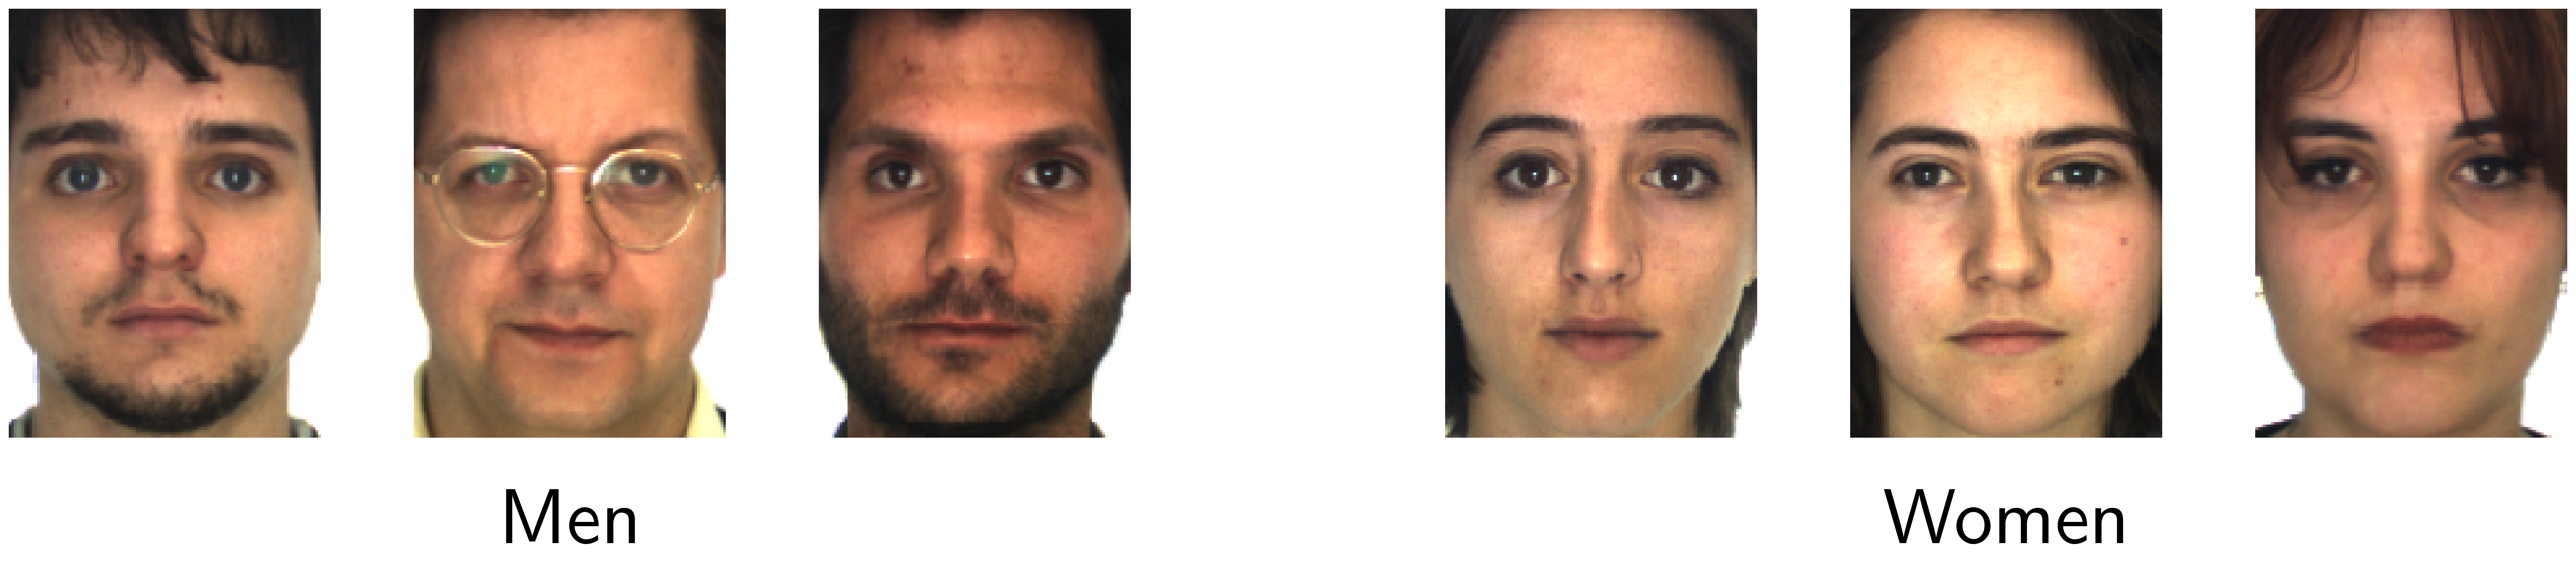
\includegraphics[scale=0.05]{ARgender_men.png}
    \end{center}
    \caption{Các ví dụ mẫu trong AR Face}
    \label{Hình 5.11}
    \end{figure}
\end{center}


 \subsection{Phương pháp trích xuất đặc trưng của tập dữ liệu}
 Đây là phương pháp trích xuất của tác giả Vũ Hữu Tiệp ở bài báo \cite{machinelearningcoban}. Trước khi đưa vào huấn luyện, các hình ảnh khuôn mặt đã được cắt lại sao cho kích thước vừa đúng với khuôn mặt ở kích thước 165x120 (pixel) bằng phương pháp PCA veus LDA \cite{machinelearningcoban}.
 Theo tác giả, mỗi bức ảnh RGB có kích thước 3x165x120 (số channels 3, chiều cao 165, chiều rộng 120) có số chiều thực sự rất lớn nên chúng ta cần phải có bước trích xuất đặc trưng phù hợp. Theo công thức về độ sáng (luminosity) chúng ta có thể chuyển ảnh màu RGB về ảnh xám (greyscale) theo công thức: 
 \begin{mybox}
 \begin{center}
       Y' = 0.299*R + 0.587*G + 0.114*B. 
 \end{center}

 \end{mybox}
 Khi chuyển ảnh màu thành ánh xám, dữ liệu của chúng ta vẫn còn là dữ liệu 2 chiều cho mỗi điểm dữ liệu, do đó chúng ta có thể làm phẳng dữ liệu dạng ma trận thành dữ liệu vector bằng phương pháp LDA( \cite{machinelearningcoban}) để thu giảm số chiều của dữ liệu về 500.\\
 Tập dataset mà nhóm sử dụng chia thành 2 tập là tập huấn luyện và tập kiểm thử. Dữ liệu huấn luyện bao gồm ảnh của 25 nam, 25 nữ ứng với 700 ảnh. Dữ liệu kiểm thử cũng tương tự nhưng là những người khác so với dữ liệu huấn luyện.  
\subsection{Ứng dụng coreset vào bài toán}
Với phần ứng dụng, ta chỉ đưa ra kết quả khi chạy với các tập coreset để cho thấy được mức độ hiệu quả của nó. Từ tập huấn luyện, ta thực hiện việc lấy các tập coreset ứng với kích thước từ 1\% đến 30\% so với tập huấn luyện. Kết quả được đánh giá dựa vào các chỉ số như: \textit{precision, recall, f1 score, accuracy score} và thời gian huấn luyện các tập coreset ứng với các kernel linear, polynomial và rbf.\\

\begin{center}
    \begin{figure}[H]
    \begin{center}
     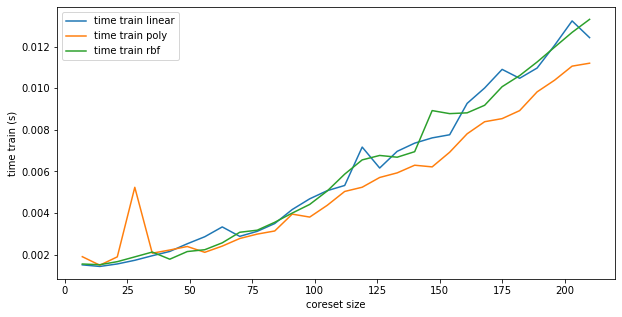
\includegraphics[scale=0.5]{timetrain_AR_gender.png}
    \end{center}
     \caption{Thời gian huấn luyện ứng của tập coreset ứng với các kernel}
    \label{Hình 5.12}
    \end{figure}
\end{center}
\begin{center}
    \begin{figure}[H]
    \begin{center}
     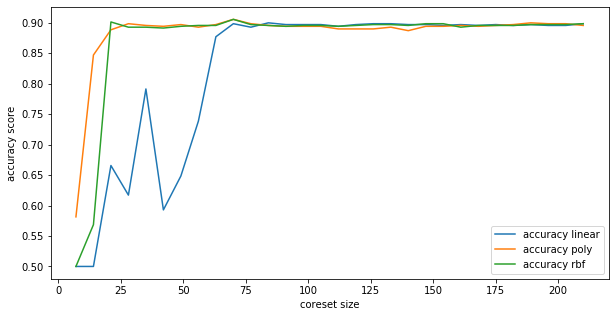
\includegraphics[scale=0.5]{accuracy_AR_gender.png}
    \end{center}
     \caption{Minh họa accuracy score của tập coreset ứng với các kernel}
    \label{Hình 5.13}
    \end{figure}
\end{center}
\begin{center}
    \begin{figure}[H]
    \begin{center}
     \includegraphics[scale=0.5]{precision_AR_gender.png}
    \end{center}
     \caption{Minh họa precision score của tập coreset ứng với các kernel}
    \label{Hình 5.14}
    \end{figure}
\end{center}
\begin{center}
    \begin{figure}[H]
    \begin{center}
     \includegraphics[scale=0.5]{recall_AR_gender.png}
    \end{center}
     \caption{Minh họa recall score của tập coreset ứng với các kernel}
    \label{Hình 5.15}
    \end{figure}
\end{center}
\begin{center}
    \begin{figure}[H]
    \begin{center}
     \includegraphics[scale=0.5]{f1_score_AR_gender.png}
    \end{center}
     \caption{Minh họa f1 score của tập coreset ứng với các kernel}
    \label{Hình 5.16}
    \end{figure}
\end{center}
Cũng như các kết quả đã được trình bày ở Chương 4 và Chương 5, một số thông số dùng để đánh giá sự hiệu quả của coreset được thể hiện thông qua các Hình \ref{Hình 5.12}, Hình \ref{Hình 5.13}, Hình \ref{Hình 5.14}, Hình \ref{Hình 5.15} và Hình \ref{Hình 5.16}. Ta thấy rằng,nếu sử dụng mô hình SVM và coreset, thì kết quả đưa ra có độ chính xác cao mặc dù ta chỉ sử dụng dưới 30\% dữ liệu tập huấn luyện, một kết quả rất tốt. Nhận diện giới tính thông qua ảnh khuôn mặt là một trong những bài toán trong lĩnh vực nhận diện hình ảnh. Qua đây cũng cho ta thấy được, coreset có thể sử dụng hiệu quả với dữ liệu ảnh. 

\newpage
\chapter{Tổng kết}
\section{Kết quả đạt được}
Trong quá trình tìm hiểu và nghiên cứu, nhóm đã thu được một số kết quả sau đây:
\begin{itemize}
    \item Nhóm đã tìm hiểu được một số kiến thức về mô hình SVM và coreset về các khía cạnh như: Cơ sở toán học, ứng dụng, ưu điểm, nhược điểm,...
    \item Nhóm đã cho thấy rằng sự hiệu quả khi sử dụng coreset trong mô hình SVM đem lại hiệu quả lớn, thời gian huấn luyện các tập coreset nhỏ hơn rất nhiều khi huấn luyện với tập dữ liệu gốc nhưng kết quả không quá chênh lệch với nhau.
    \item Nhóm cũng đã vận dụng việc kết hợp coreset và mô hình SVM trong 2 bài toán thực tế là bài toán phòng chống gian lận và bài toán nhận diện giới tính dựa vào ảnh khuôn mặt.
\end{itemize}
Với những kết quả đạt được, tuy vẫn gặp nhiều tồn tại và hạn chế, tuy nhiên nhóm đã hoàn thành những nhiệm vụ và mục tiêu đã được đề ra.

\section{Nhược điểm}
Trong quá trình làm đề tài, nhóm gặp một số hạn chế sau:
\begin{itemize}
    \item Mặc dù luận văn đã cho ta thấy được sự hiệu quả của coreset và mô hình SVM trong bài toán phân loại. Tuy nhiên, việc lấy coreset mất khá nhiều thời gian, thậm chí lâu hơn việc huấn luyện tập dữ liệu gốc.
    \item Hiện tại, nhóm mới chỉ áp dụng coreset và mô hình SVM cho các tập dữ liệu số, chưa áp dụng cho các tập dữ liệu khác như âm thanh, văn bản,...
    \item Trong quá trình làm, nhóm chỉ hiện thực lại giải thuật ProTras mà chưa có sự tối ưu trong đó.
    \item Tài nguyên máy tính còn hạn chế.
\end{itemize}
\section{Cải tiến trong tương lai}
Trong quá trình làm đề tài, nhóm nhìn thấy có một số vấn đề có thể cải tiến được như sau:
\begin{itemize}
    \item Về mặt thời gian, đây là một nhược điểm khi lấy coreset, vì vậy ta có thể cải tiến bằng cách kết hợp các giải thuật hoặc các phương pháp xử lý song song để tăng tốc độ lấy coreset hơn.
    \item Hiện tại giải thuật coreset mới chỉ được vận dụng với những dữ liệu số, ta có thể vận dụng coreset với các kiểu dữ liệu khác nhau như âm thanh, văn bản...
    \item Ta còn có thể cải thiện thuật toán lấy coreset sao cho lấy coreset với độ chính xác cao, thể hiện được đầy đủ tính chất của tập gốc bằng cách áp dụng các công thức tính khoảng cách khác nhau,... 
\end{itemize}
%%%%%%%%%%%%%%%%%%%%%%%%%%%%%%%%%

\begin{thebibliography}{80}
\bibitem{machinelearningcoban}
https://machinelearningcoban.com - lần truy cập cuối cùng 15/07/2020
\bibitem{Small Coresets to Represent Large Training Data for Support Vector Machines}
Cenk Baykal, Murad Tukan, Dan Feldman, Daniela Rus, \textit{Small Coresets to Represent Large Training Data for Support Vector Machines} 
\bibitem{Core Vector Machines: Fast SVM Training on Very Large Data Sets}
Ivor W. Tsang, James T. Kwok, Pak-Ming Cheung, \textit{Core Vector Machines: Fast SVM Training on Very Large Data Sets}
\bibitem{Geometric Approximation via Coresets}
Pankaj K. Agarwal, Sariel Har-Peled, Kasturi R. Varadaraja, \textit{Geometric Approximation via Coresets}
\bibitem{Voice Gender Dataset}
https://www.kaggle.com - lần truy cập cuối cùng 20/07/2020
\bibitem{Credit Card Dataset}
https://archive.ics.uci.edu/ml/datasets/default+of+credit+card+clients - lần truy cập cuối cùng 20/07/2020
\bibitem{AR origin}
http://www2.ece.ohio-state.edu/~aleix/ARdatabase.html - lần truy cập cuối cùng 20/07/2020
\bibitem{Color Database}
https://www.nist.gov/programs-projects/face-projects/colorferet/request.html - lần truy cập cuối cùng 20/07/2020
\bibitem{Face Database}
http://agingmind.utdallas.edu/facedb/ - lần truy cập cuối cùng 25/07/2020

\end{thebibliography}
%%%%%%%%%%%%%%%%%%%%%%%%%%%%%%%%%

\end{document}

